\documentclass{beamer}
\usepackage{subfigure}
%\usepackage{english}
\usepackage{graphics}
\usepackage{color}
\usepackage{textcomp}
\usepackage{url}
\graphicspath{./pics/}
% \usetheme{INET}

\usepackage{beamerthemeshadow}
% \beamersetuncovermixins{\opaqueness<1>{25}}{\opaqueness<2->{15}}

\title{Ringmap Capturing Stack for High Performance Packet Capturing in FreeBSD}
\author[Alexander Fiveg]{ Alexander Fiveg \\
\url{afiveg@freebsd.org} }
% \institute[TU Berlin/DT Labs]{Technische Universtit\"at Berlin \\ Deutsche Telekom Laboratories}

\begin{document}
\frame{\titlepage}

% Inhaltsverzeichnis
\section*{Outline}

\begin{frame}
\frametitle{Outline}
\tableofcontents
\end{frame}


%%%%%%%%%%%%%%%%%%%%%%%%%%%%%%%%%%%%%%%%%%%%%%%%%%%%%%%%%%%%%%%%%%%%%%%%%%%%%%%%%%%%%%%%%%%%%%%%%%%


% Worum es geht. Definition of Terms
\section{Motivation}

%%%%%%%%%%%%%%%%%%%%%%%%%%%%%%%%%%%%%%%%%%%%%%%%%%%%%%%%%%%%%%%%%%%
\begin{frame}
	\begin{center}
	\huge{Motivation}
	\end{center}
\end{frame}

%%%%%%%%%%%%%%%%%%%%%%%%%%%%%%%%%%%%%%%%%%%%%%%%%%%%%%%%%%%%%%%%%%%
\subsection*{Problem}
\begin{frame}
\frametitle{Problem}
\textbf{Problems arising during packet capturing:}
\begin{itemize}
	\item High bit rates and packet rates
		\begin{itemize}
			\item [$\Rightarrow$] \textcolor{red}{high CPU load and packet loss} \newline
		\end{itemize}
\end{itemize}
\begin{figure}[H] 
	\subfigure{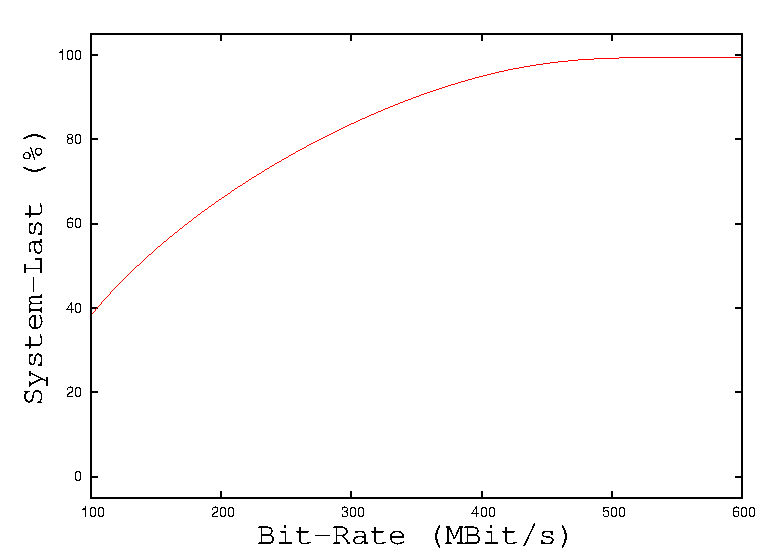
\includegraphics [width=0.45\textwidth]{plots/sysload_generic_slide}}
	\subfigure{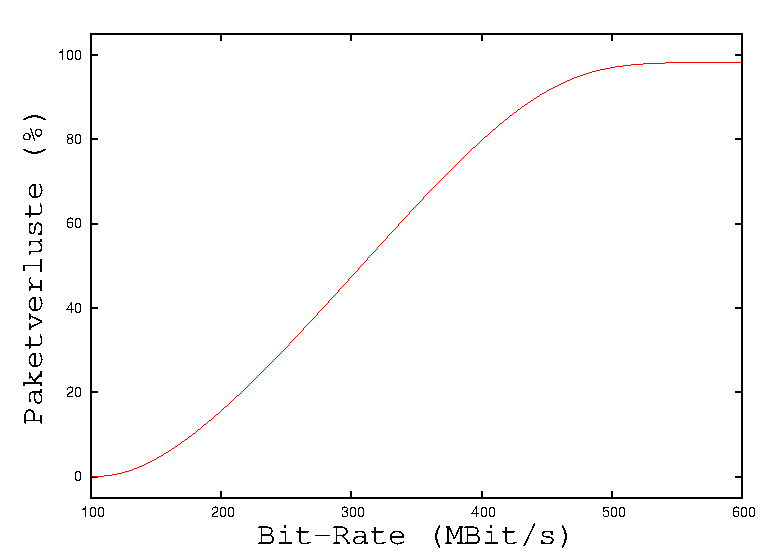
\includegraphics [width=0.45\textwidth]{plots/pktlos_generic_slide}}
	\caption{Capturing 64-Bytes packets. (Bezier curves)}
\end{figure}
\end{frame}

\subsection*{The cause of the Problems}
%%%%%%%%%%%%%%%%%%%%%%%%%%%%%%%%%%%%%%%%%%%%%%%%%%%%%%%%%%%%%%%%%%%
\begin{frame}
\frametitle{The reason of the Problems}
\textbf{Inefficiency of standard capturing software}\newline
\begin{itemize}
	\item To many ``expensive'' operations in terms of CPU cycles: 
\begin{itemize}
			\item System calls
			\item Packet copy operations
			\item Memory allocations
			\item etc\ldots\newline
\end{itemize}
% \begin{small}
% 	\item [$\Rightarrow$] probably the capturing software for FreeBSD was
% 		developed at a time when  network data-rates were low enough relative
% 		to hardware processing resources such that capturing loss problems did
% 		not arise?
% \end{small}
\end{itemize}
\end{frame}

\subsection*{Goal of the Project}
%%%%%%%%%%%%%%%%%%%%%%%%%%%%%%%%%%%%%%%%%%%%%%%%%%%%%%%%%%%%%%%%%%%
\begin{frame}
\frametitle{Goal of the project}
%\begin{large}
\textbf{Increase the capturing performance in FreeBSD}
	\begin{itemize}
		\item Design and implementation the new capturing software to
			minimize the \textbf{packet loss} and \textbf{CPU load} during capturing. \newline \newline
	\end{itemize}
%\begin{large}
\textbf{Supported Hardware:}
%\end{large}
\begin{itemize}
	\item The following \emph{Intel GbE Controllers:}
		\begin{itemize}
			\item \small{\emph{8254x, 8257x, 8259x}}
		\end{itemize}
%	\item Software:	\emph{FreeBSD}
\end{itemize}
\end{frame}

%%%%%%%%%%%%%%%%%%%%%%%%%%%%%%%%%%%%%%%%%%%%%%%%%%%%%%%%%%%%%%%%%%%
\begin{frame}
\frametitle{Approach}
\begin{itemize}
	\item<1-> Eliminating the packet copy operations
		\begin{itemize}
			\item<1-> by using shared memory buffers (\emph{memory \textbf{mapping}})\newline
		\end{itemize}
	\item<1-> Eliminating the memory allocations
		\begin{itemize}
			\item<1-> by using \textbf{ring} buffers\newline \newline
		\end{itemize}
	\item<2->[$\Rightarrow$] $ring + mapping = \textbf{ringmap}$
\end{itemize}
\end{frame}

\section{Background}
%%%%%%%%%%%%%%%%%%%%%%%%%%%%%%%%%%%%%%%%%%%%%%%%%%%%%%%%%%%%%%%%%%%
\begin{frame}
	\begin{center}
	\huge{Background}
	\end{center}
\end{frame}

%%%%%%%%%%%%%%%%%%%%%%%%%%%%%%%%%%%%%%%%%%%%%%%%%%%%%%%%%%%%%%%%%%%
\begin{frame}
\frametitle{Packet Capturing: Hardware View}
\begin{columns}
\column[t]{0.5\textwidth}
\vspace{-15em}
\begin{enumerate}
	\item \textbf{Receiving} network packets
		\begin{itemize}
			\item receive at network adapter
			\item DMA transfer in RAM \newline
		\end{itemize}
	\item \textbf{Filtering} the received packets 
		\begin{itemize}
			\item \emph{Berkeley Packet Filter}\newline
		\end{itemize}
	\item \textbf{Storing} to the hard disk
		\begin{itemize}
			\item using a system call
		\end{itemize}
\end{enumerate}
\column[t]{0.5\textwidth}
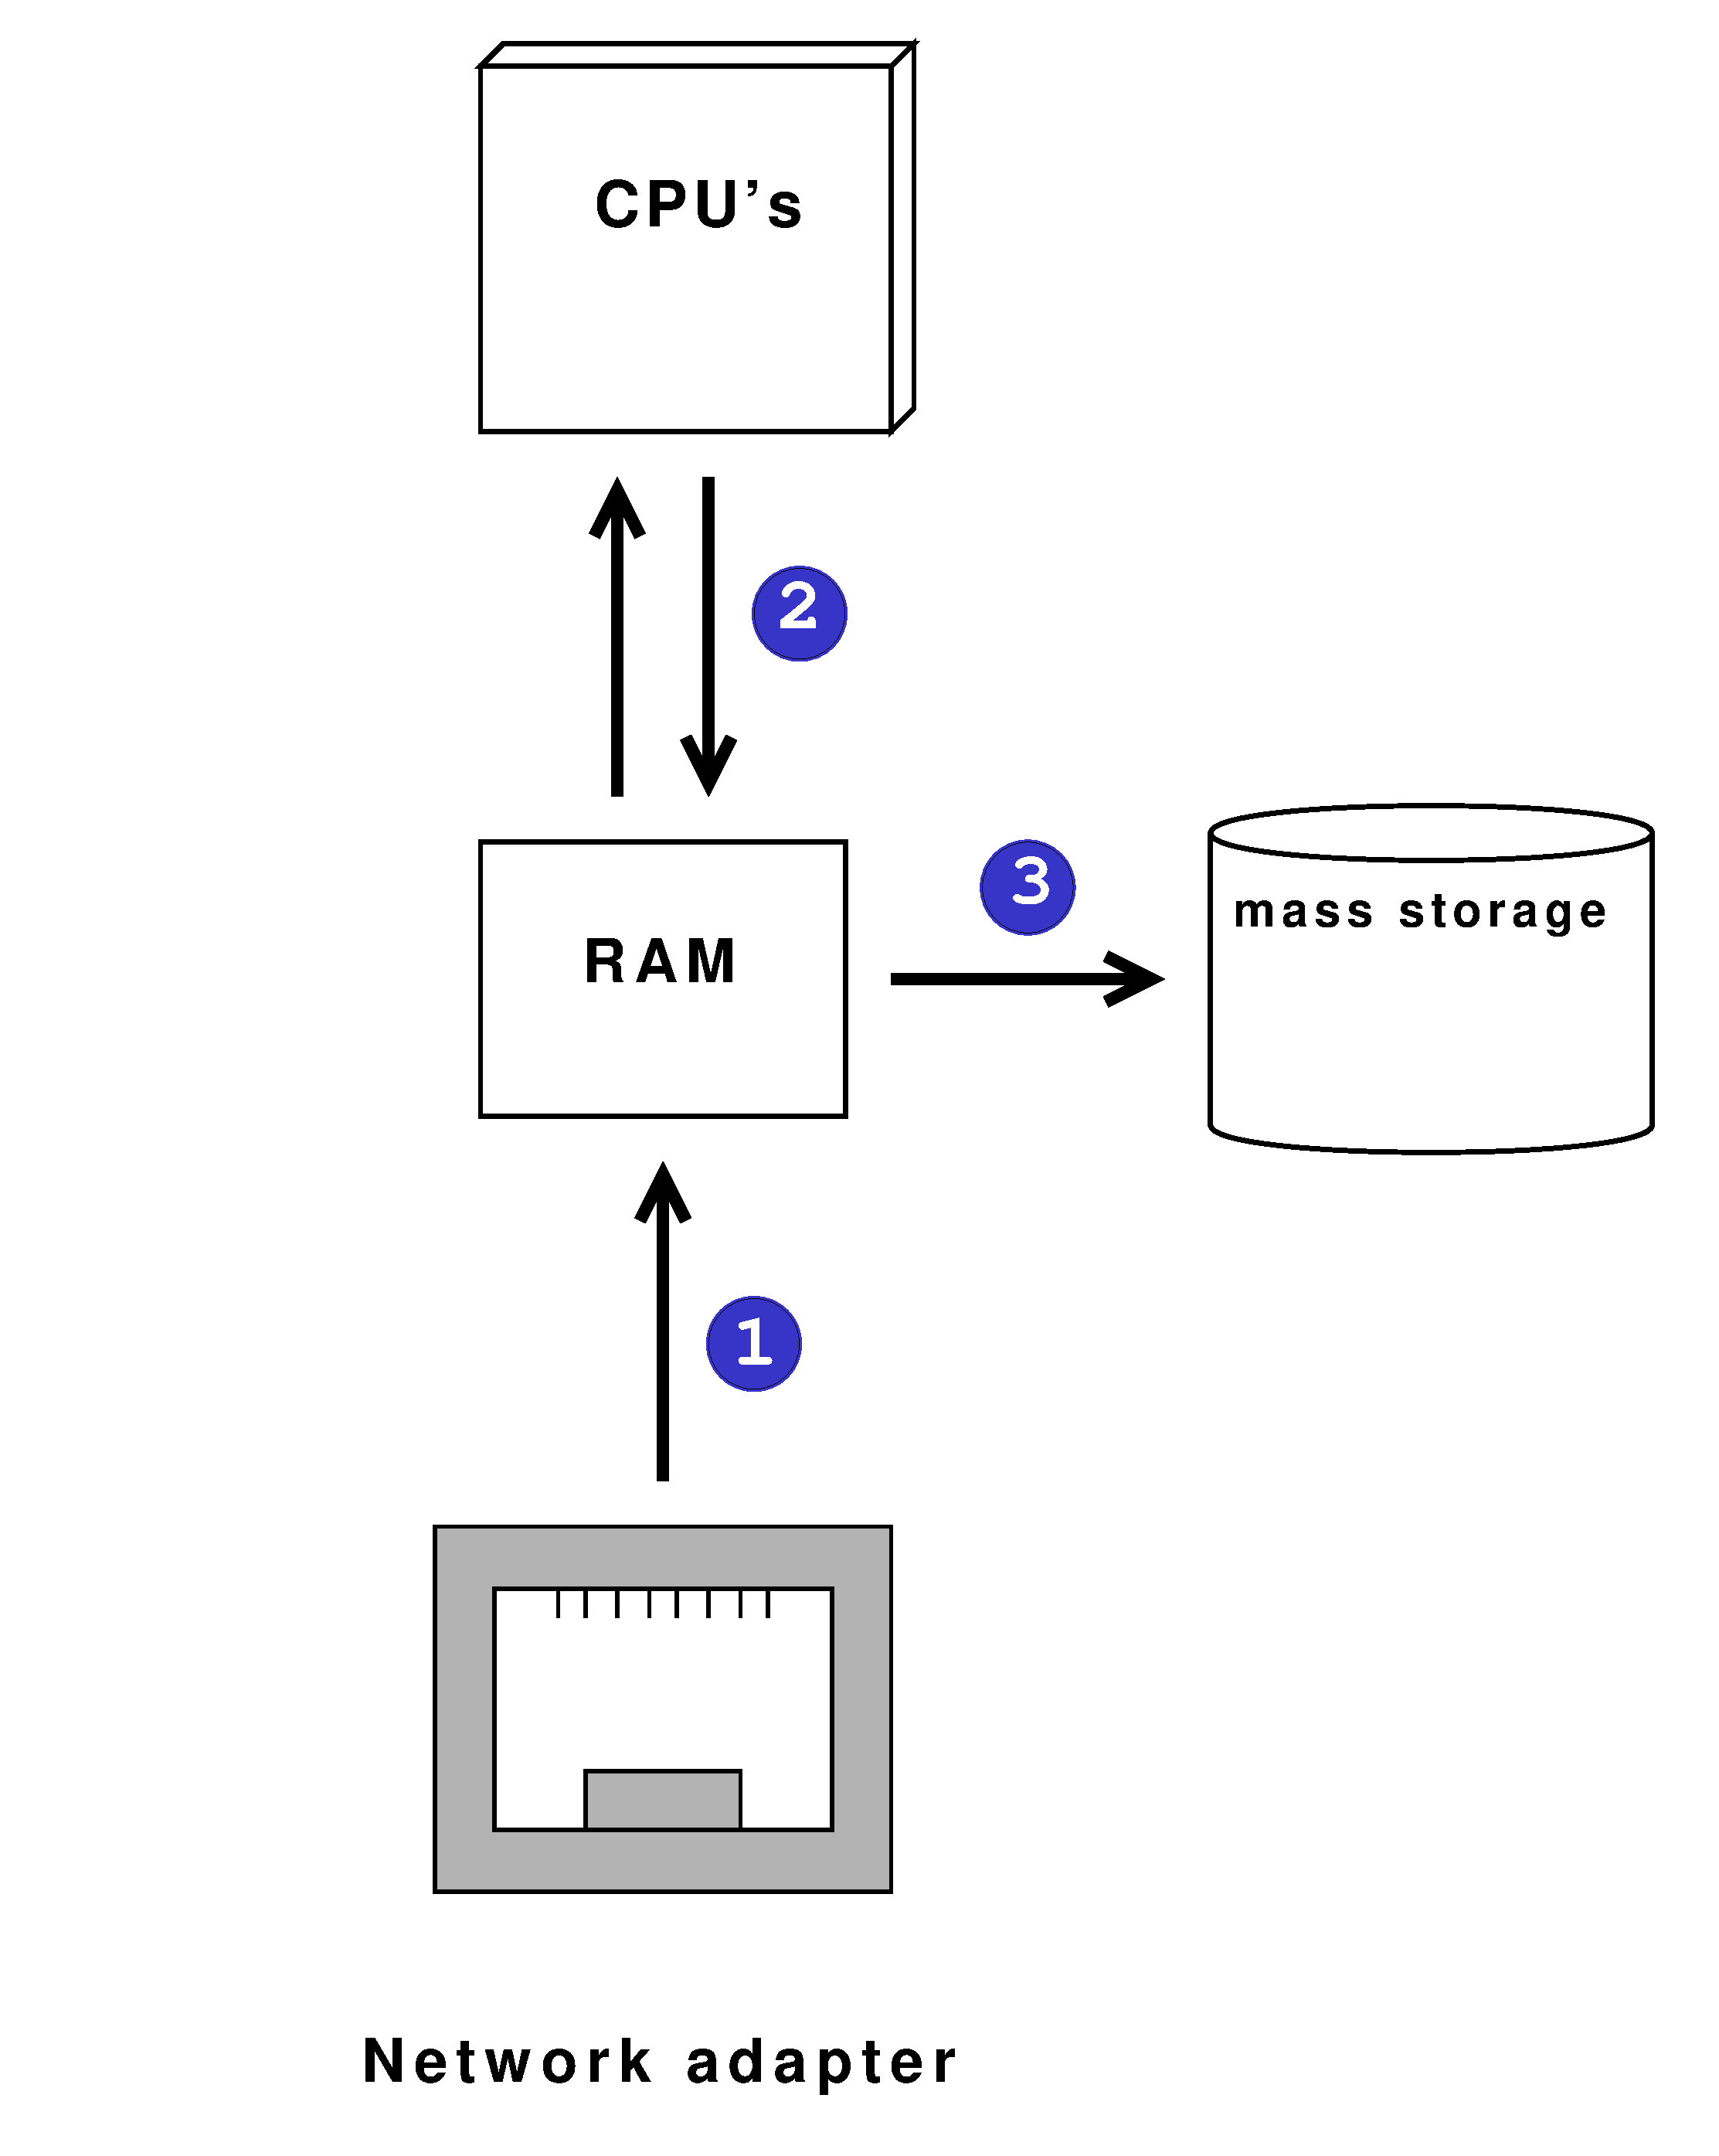
\includegraphics [width=0.82\textwidth, keepaspectratio]{pics/HardwareView}
\end{columns}
\end{frame}

%%%%%%%%%%%%%%%%%%%%%%%%%%%%%%%%%%%%%%%%%%%%%%%%%%%%%%%%%%%%%%%%%%%
\begin{frame}
\frametitle{FreeBSD Packet Capturing Stack}
\begin{itemize}
	\item \textbf{Network driver}
		\begin{itemize}
			\item Receiving packets\newline
		\end{itemize}
	\item \textbf{Berkley Packet Filter} (BPF)
		\begin{itemize}
			\item Filtering packets\newline
		\end{itemize}
	\item \textbf{User-space application}
		\begin{itemize}
			\item Accessing received packets
			\item Initiates:
				\begin{itemize}
					\item Storing packets to hard drive
					\item Output packets information to the terminal
				\end{itemize}
		\end{itemize}
\end{itemize}
\end{frame}

\subsection*{Capturing}
%%%%%%%%%%%%%%%%%%%%%%%%%%%%%%%%%%%%%%%%%%%%%%%%%%%%%%%%%%%%%%%%%%%
\begin{frame}
	\begin{center}
	\huge{How does standard packet capturing works}
	\end{center}
\end{frame}


%%%%%%%%%%%%%%%%%%%%%%%%%%%%%%%%%%%%%%%%%%%%%%%%%%%%%%%%%%%%%%%%%%%
\begin{frame}
\frametitle{FreeBSD Standard Packet Capturing Stack}
\begin{columns}
\column[t]{0.5\textwidth}
\vspace{0em}
\newline
\begin{itemize}
\item <6-> Access packets
\item <5-> Packet filtering
\item <4-> Interrupt Service Routine
\item <3-> Interrupt
\item <2-> DMA-Transfer
\item <1-> Packet is received and saved in Adapter-FIFO
\end{itemize}
\column[t]{0.5\textwidth}
\vspace{-2em}
\begin{figure}
	\only<1>{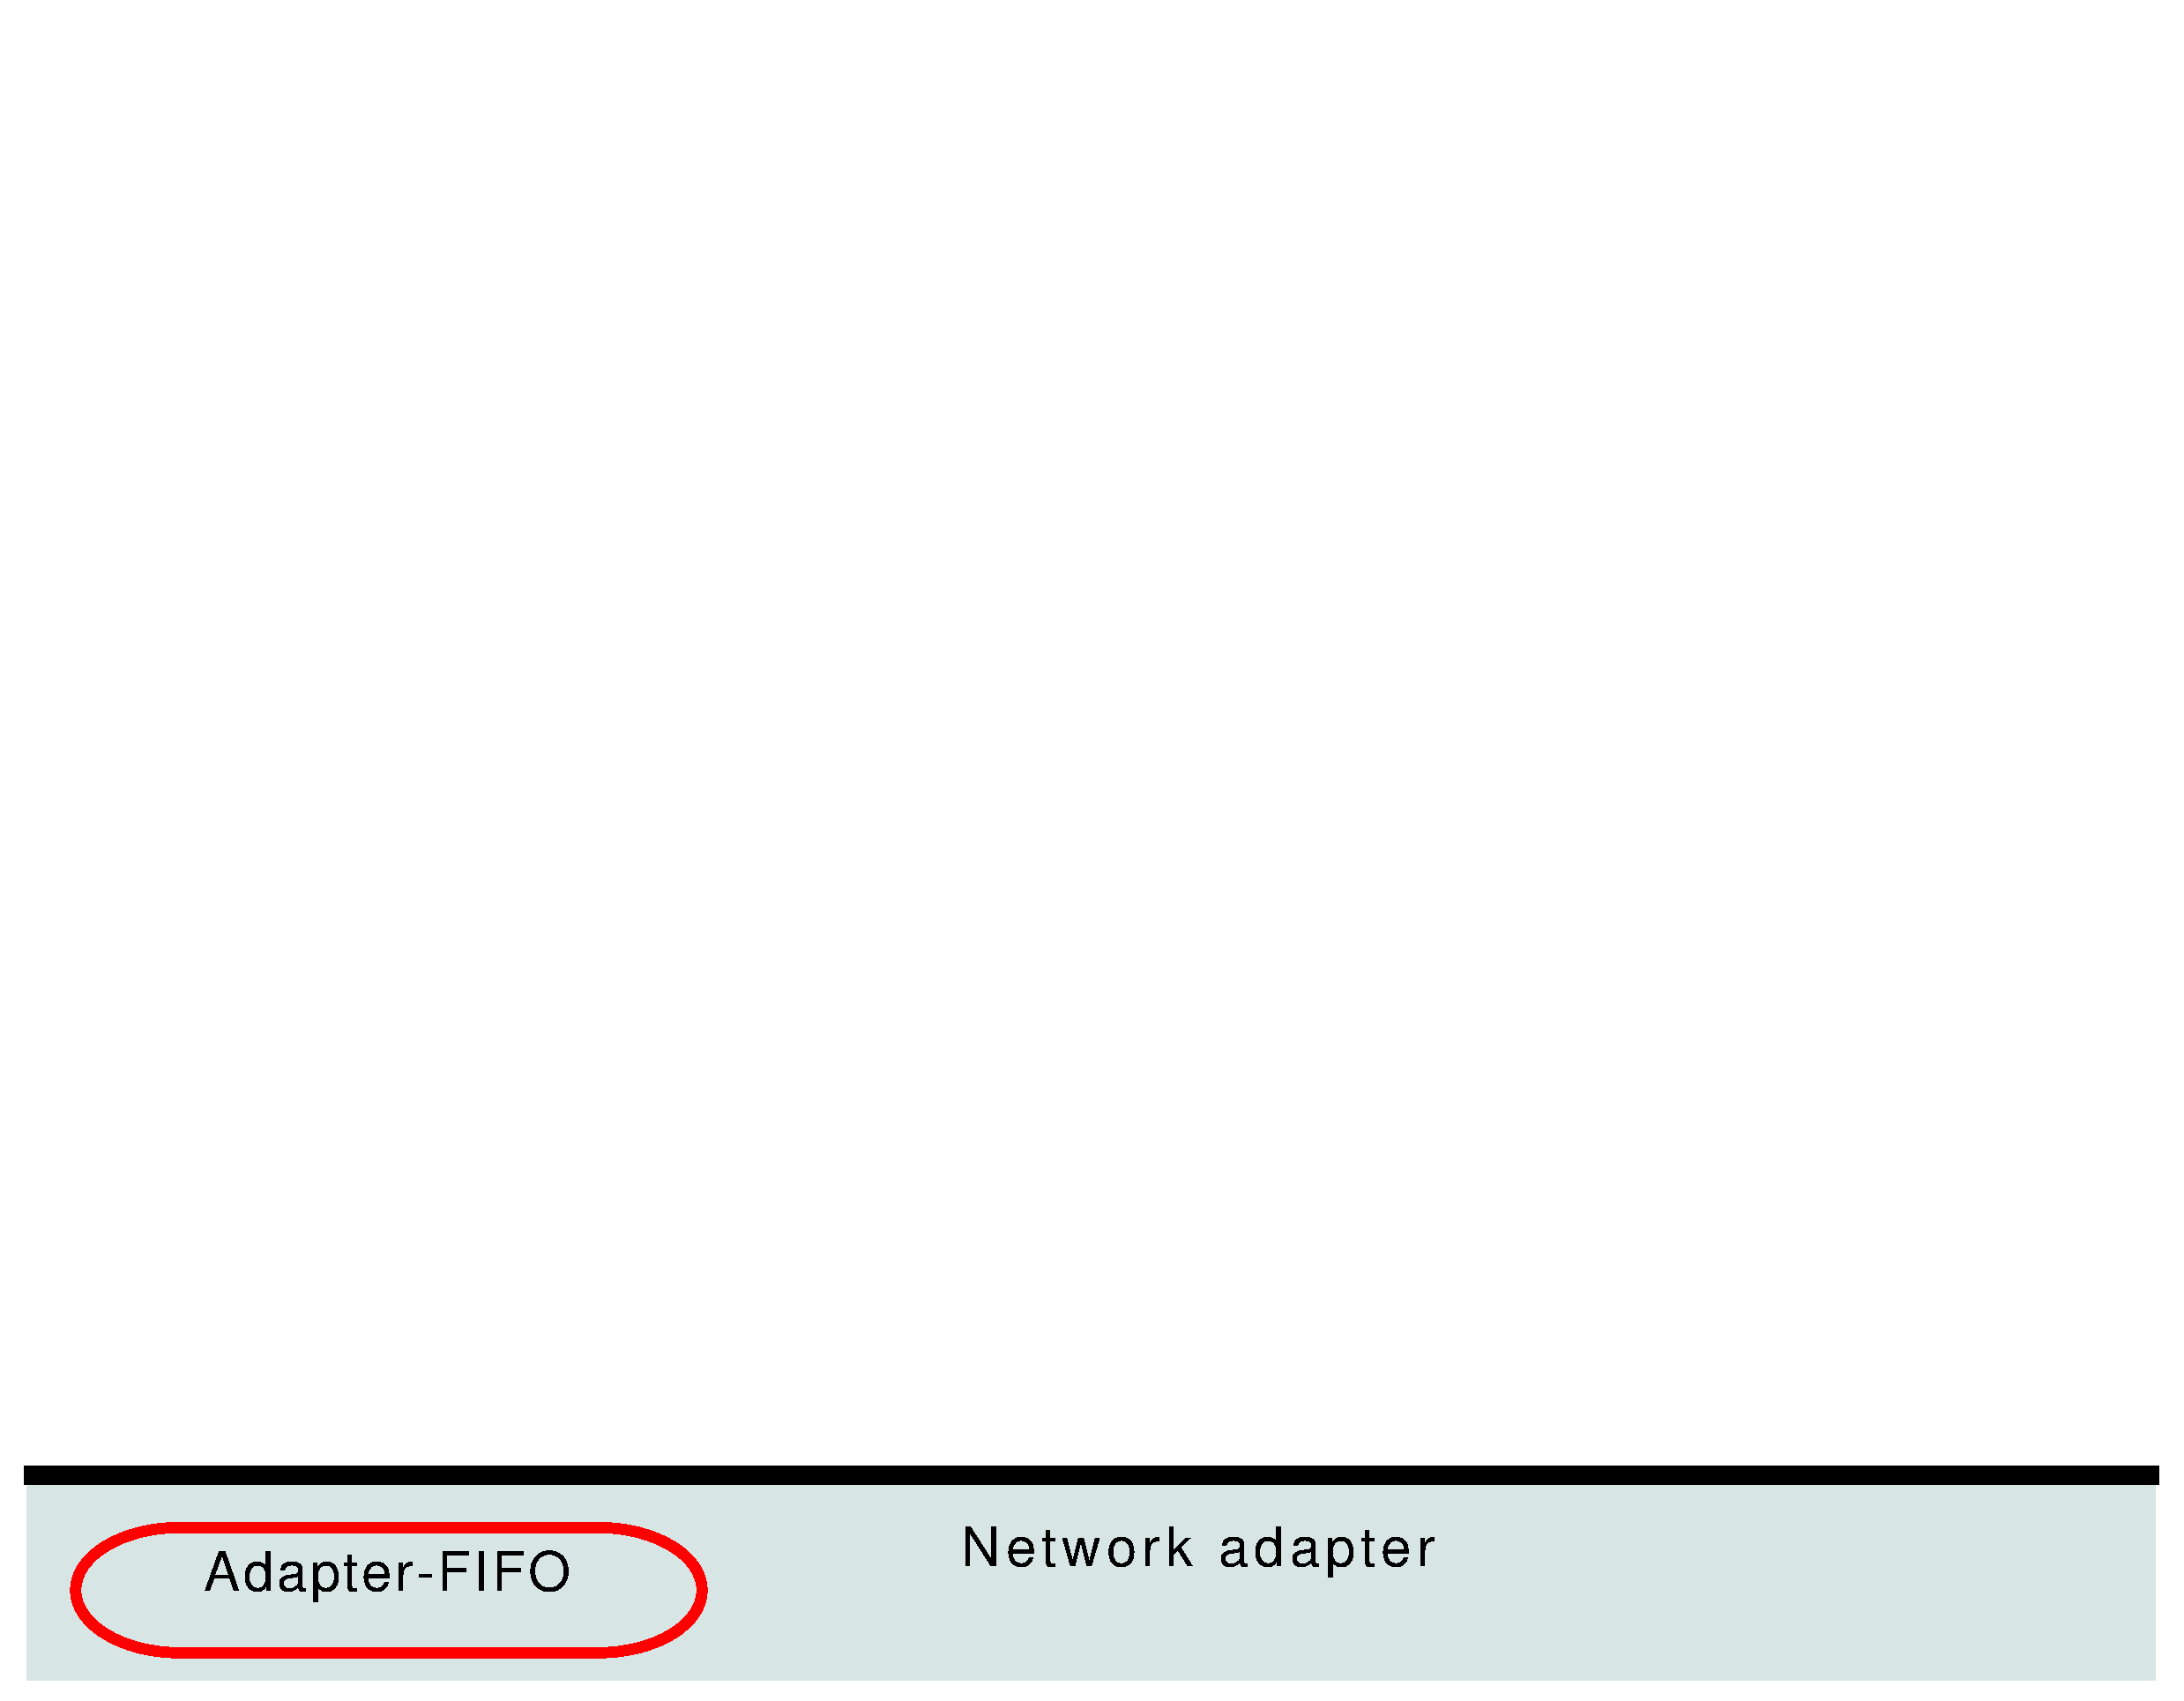
\includegraphics [height=55mm,width=60mm]{pics/3copy_0}}
	\only<2>{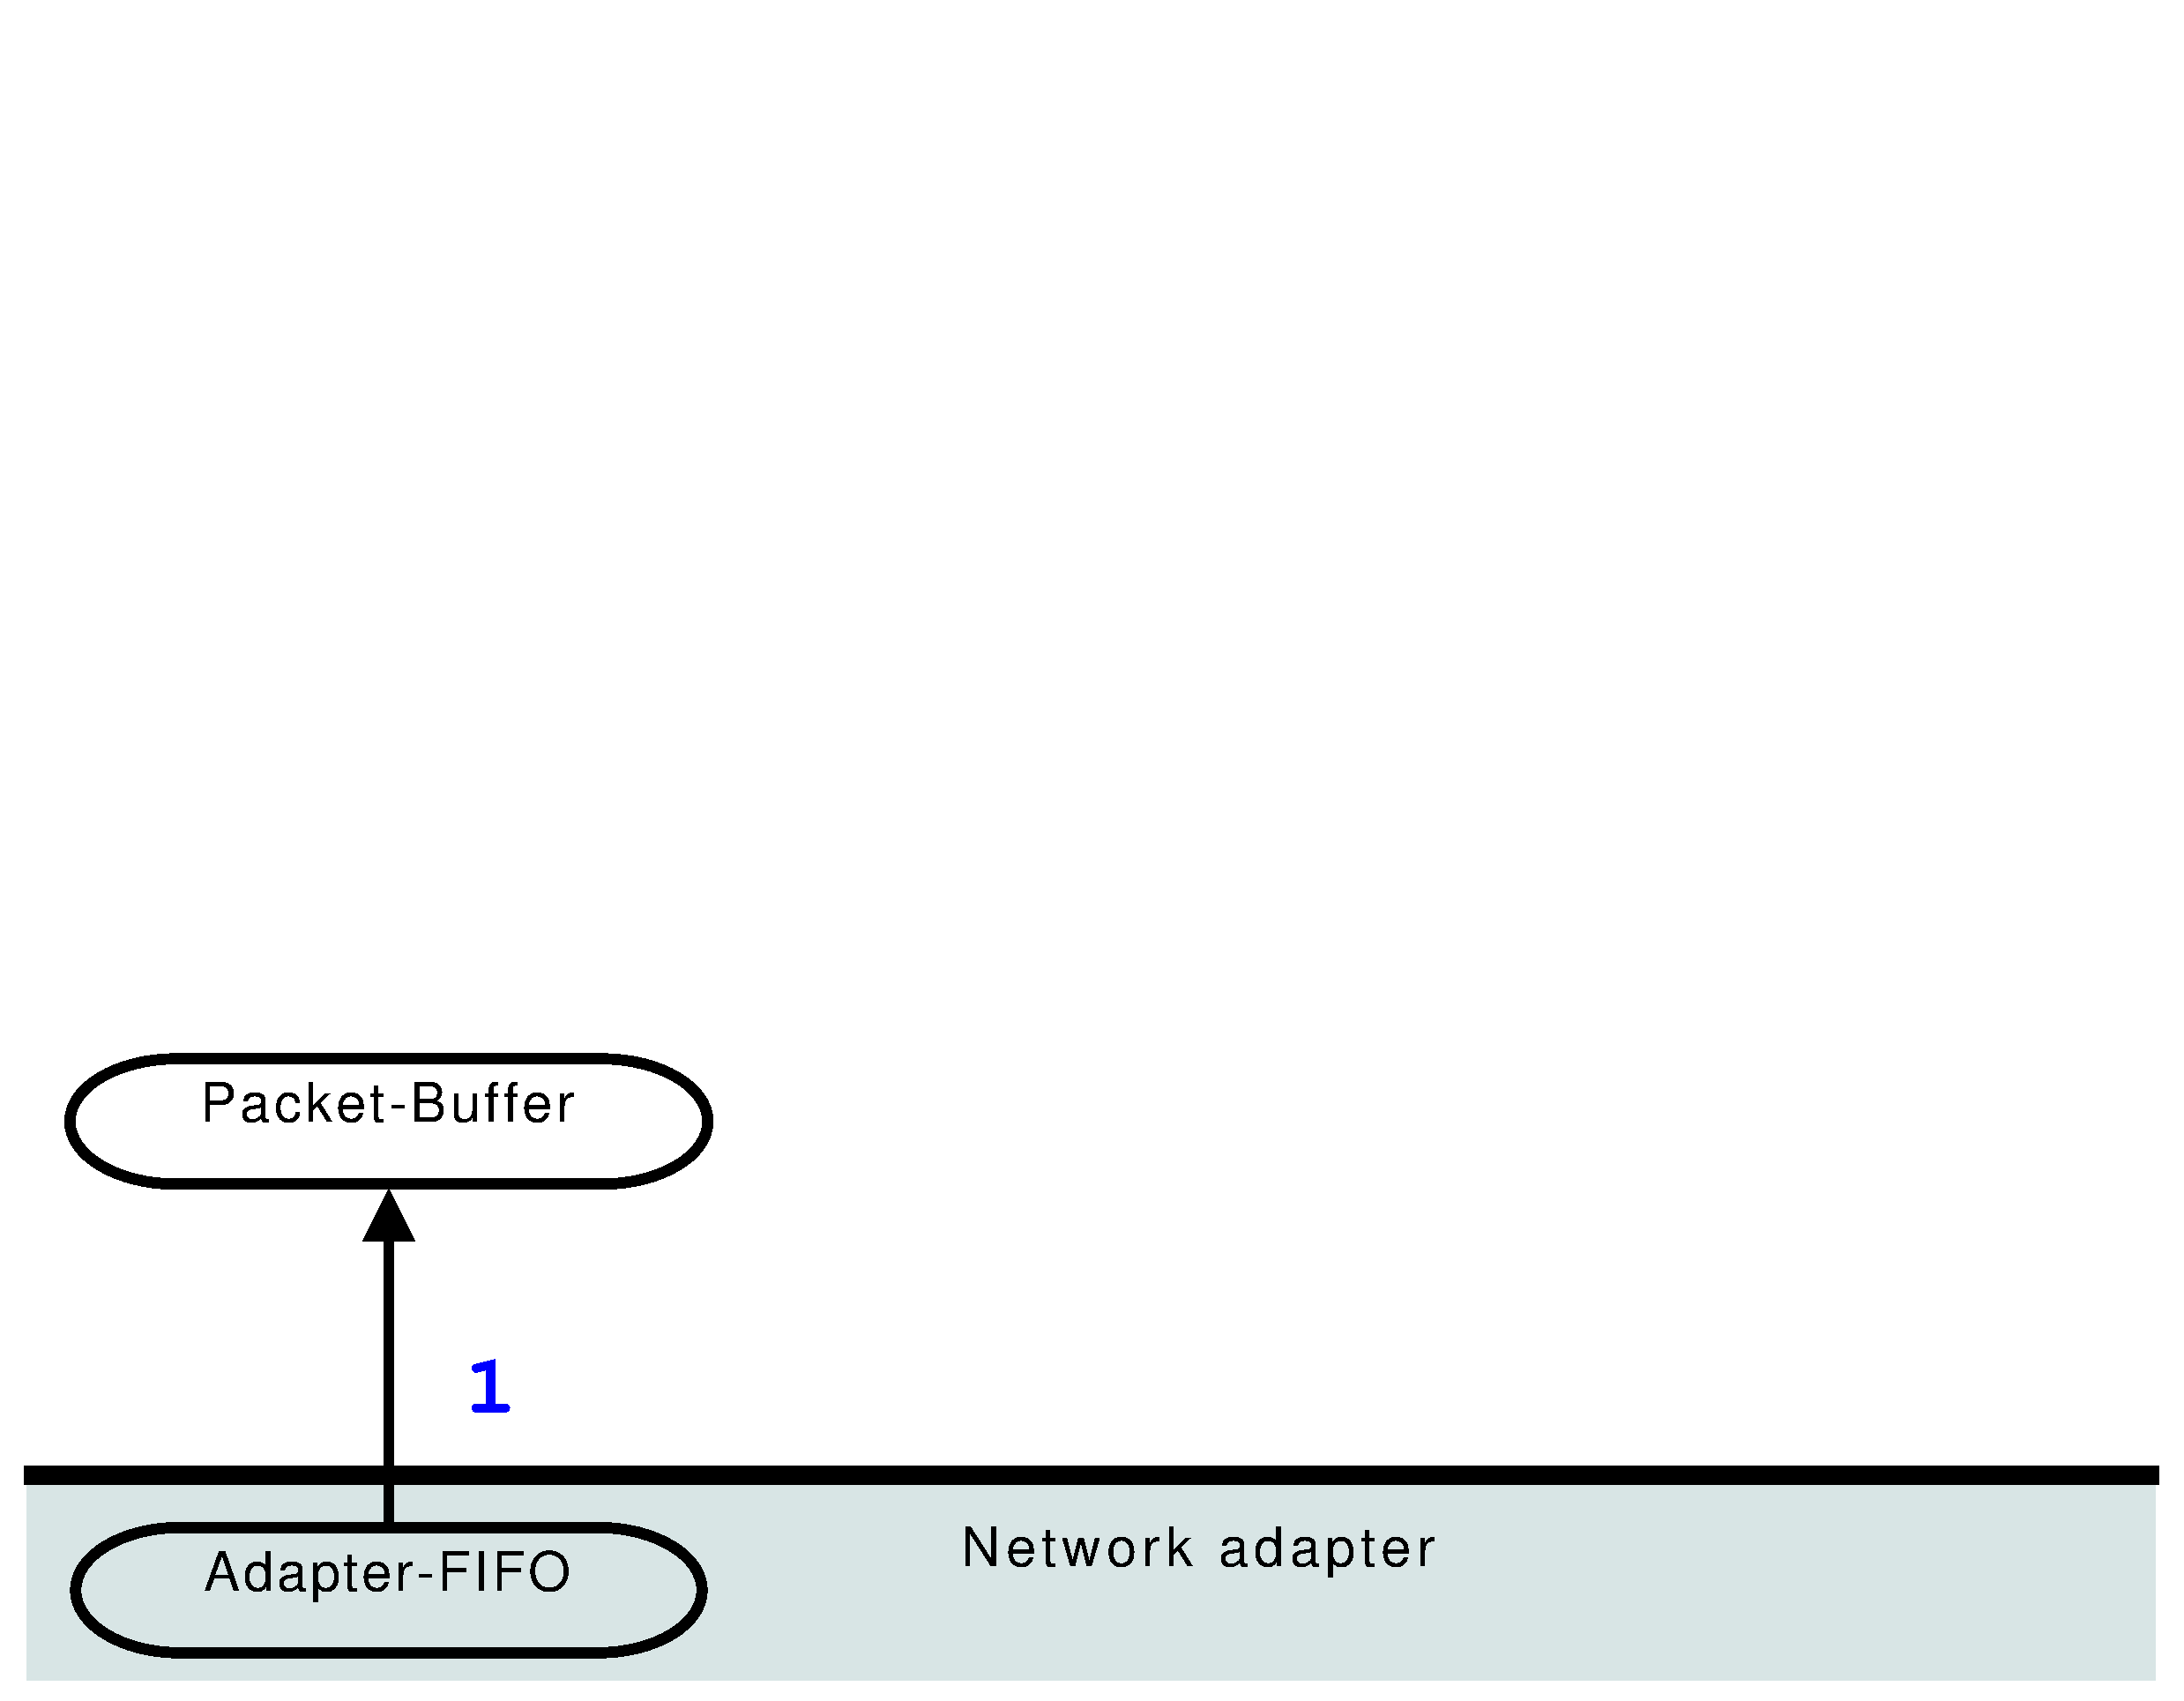
\includegraphics [height=55mm,width=60mm]{pics/3copy_0.5.eps}}
	\only<3>{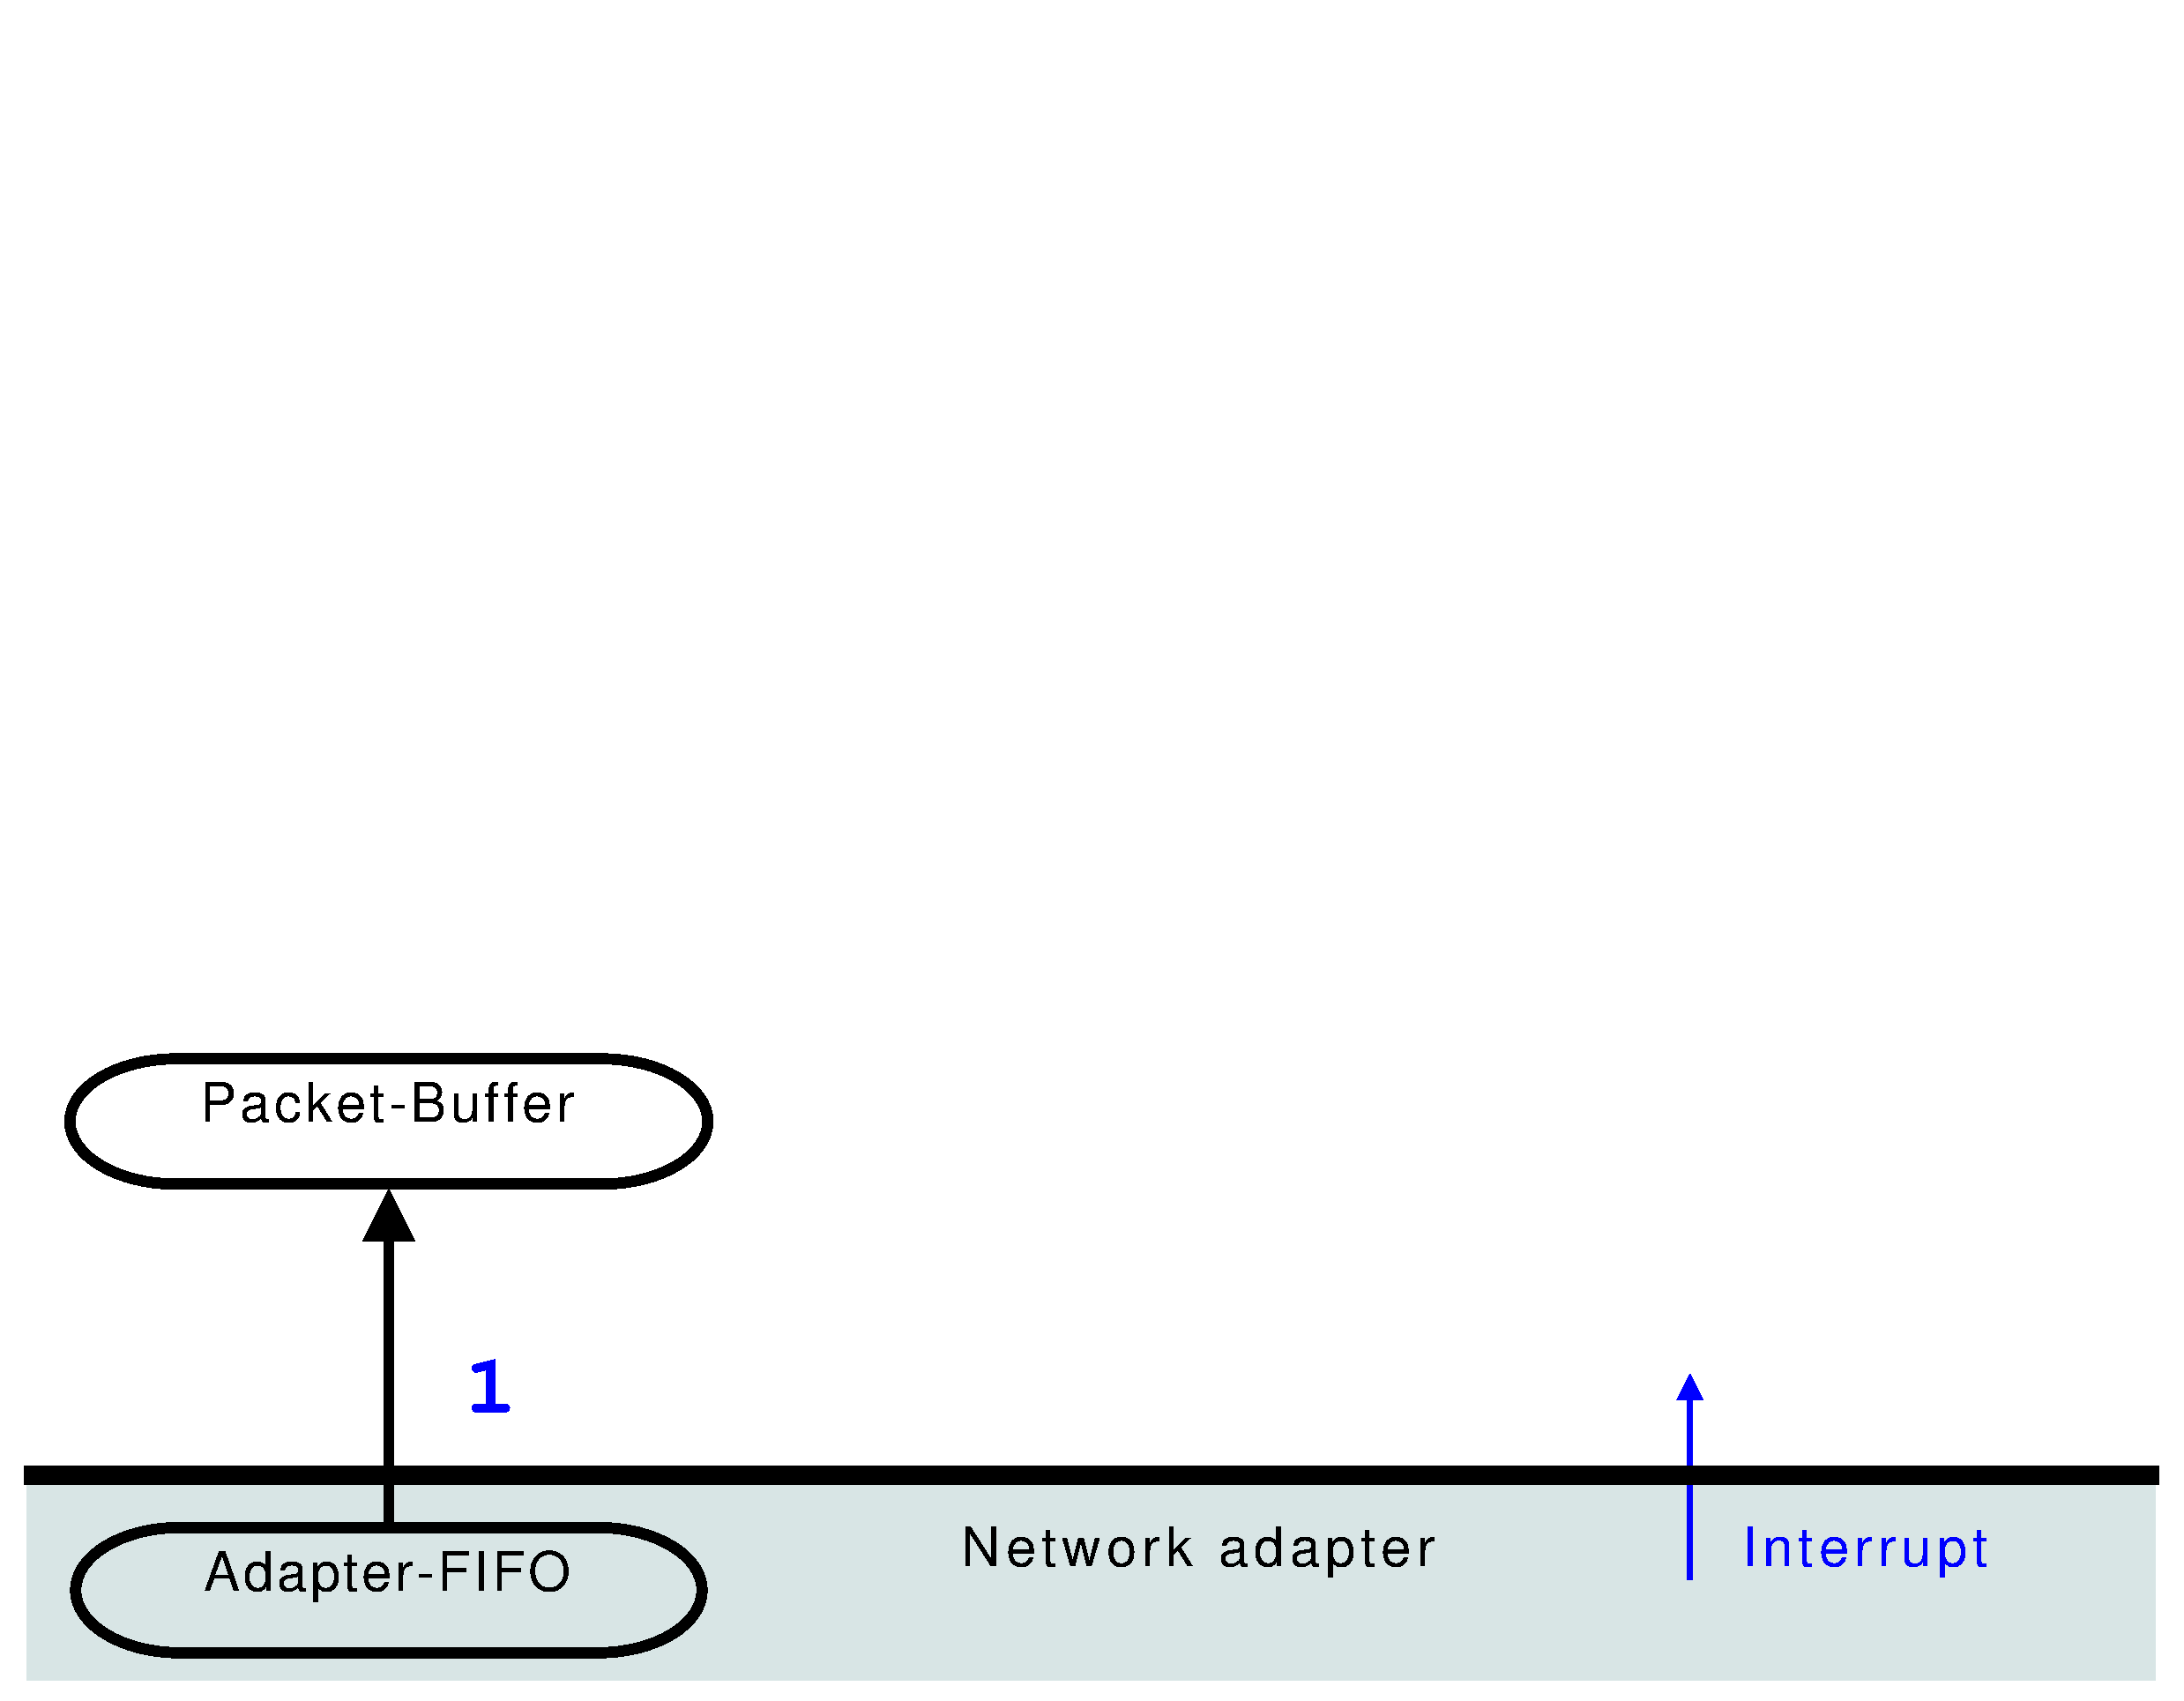
\includegraphics [height=55mm,width=60mm]{pics/3copy_0.7.eps}}
	\only<4>{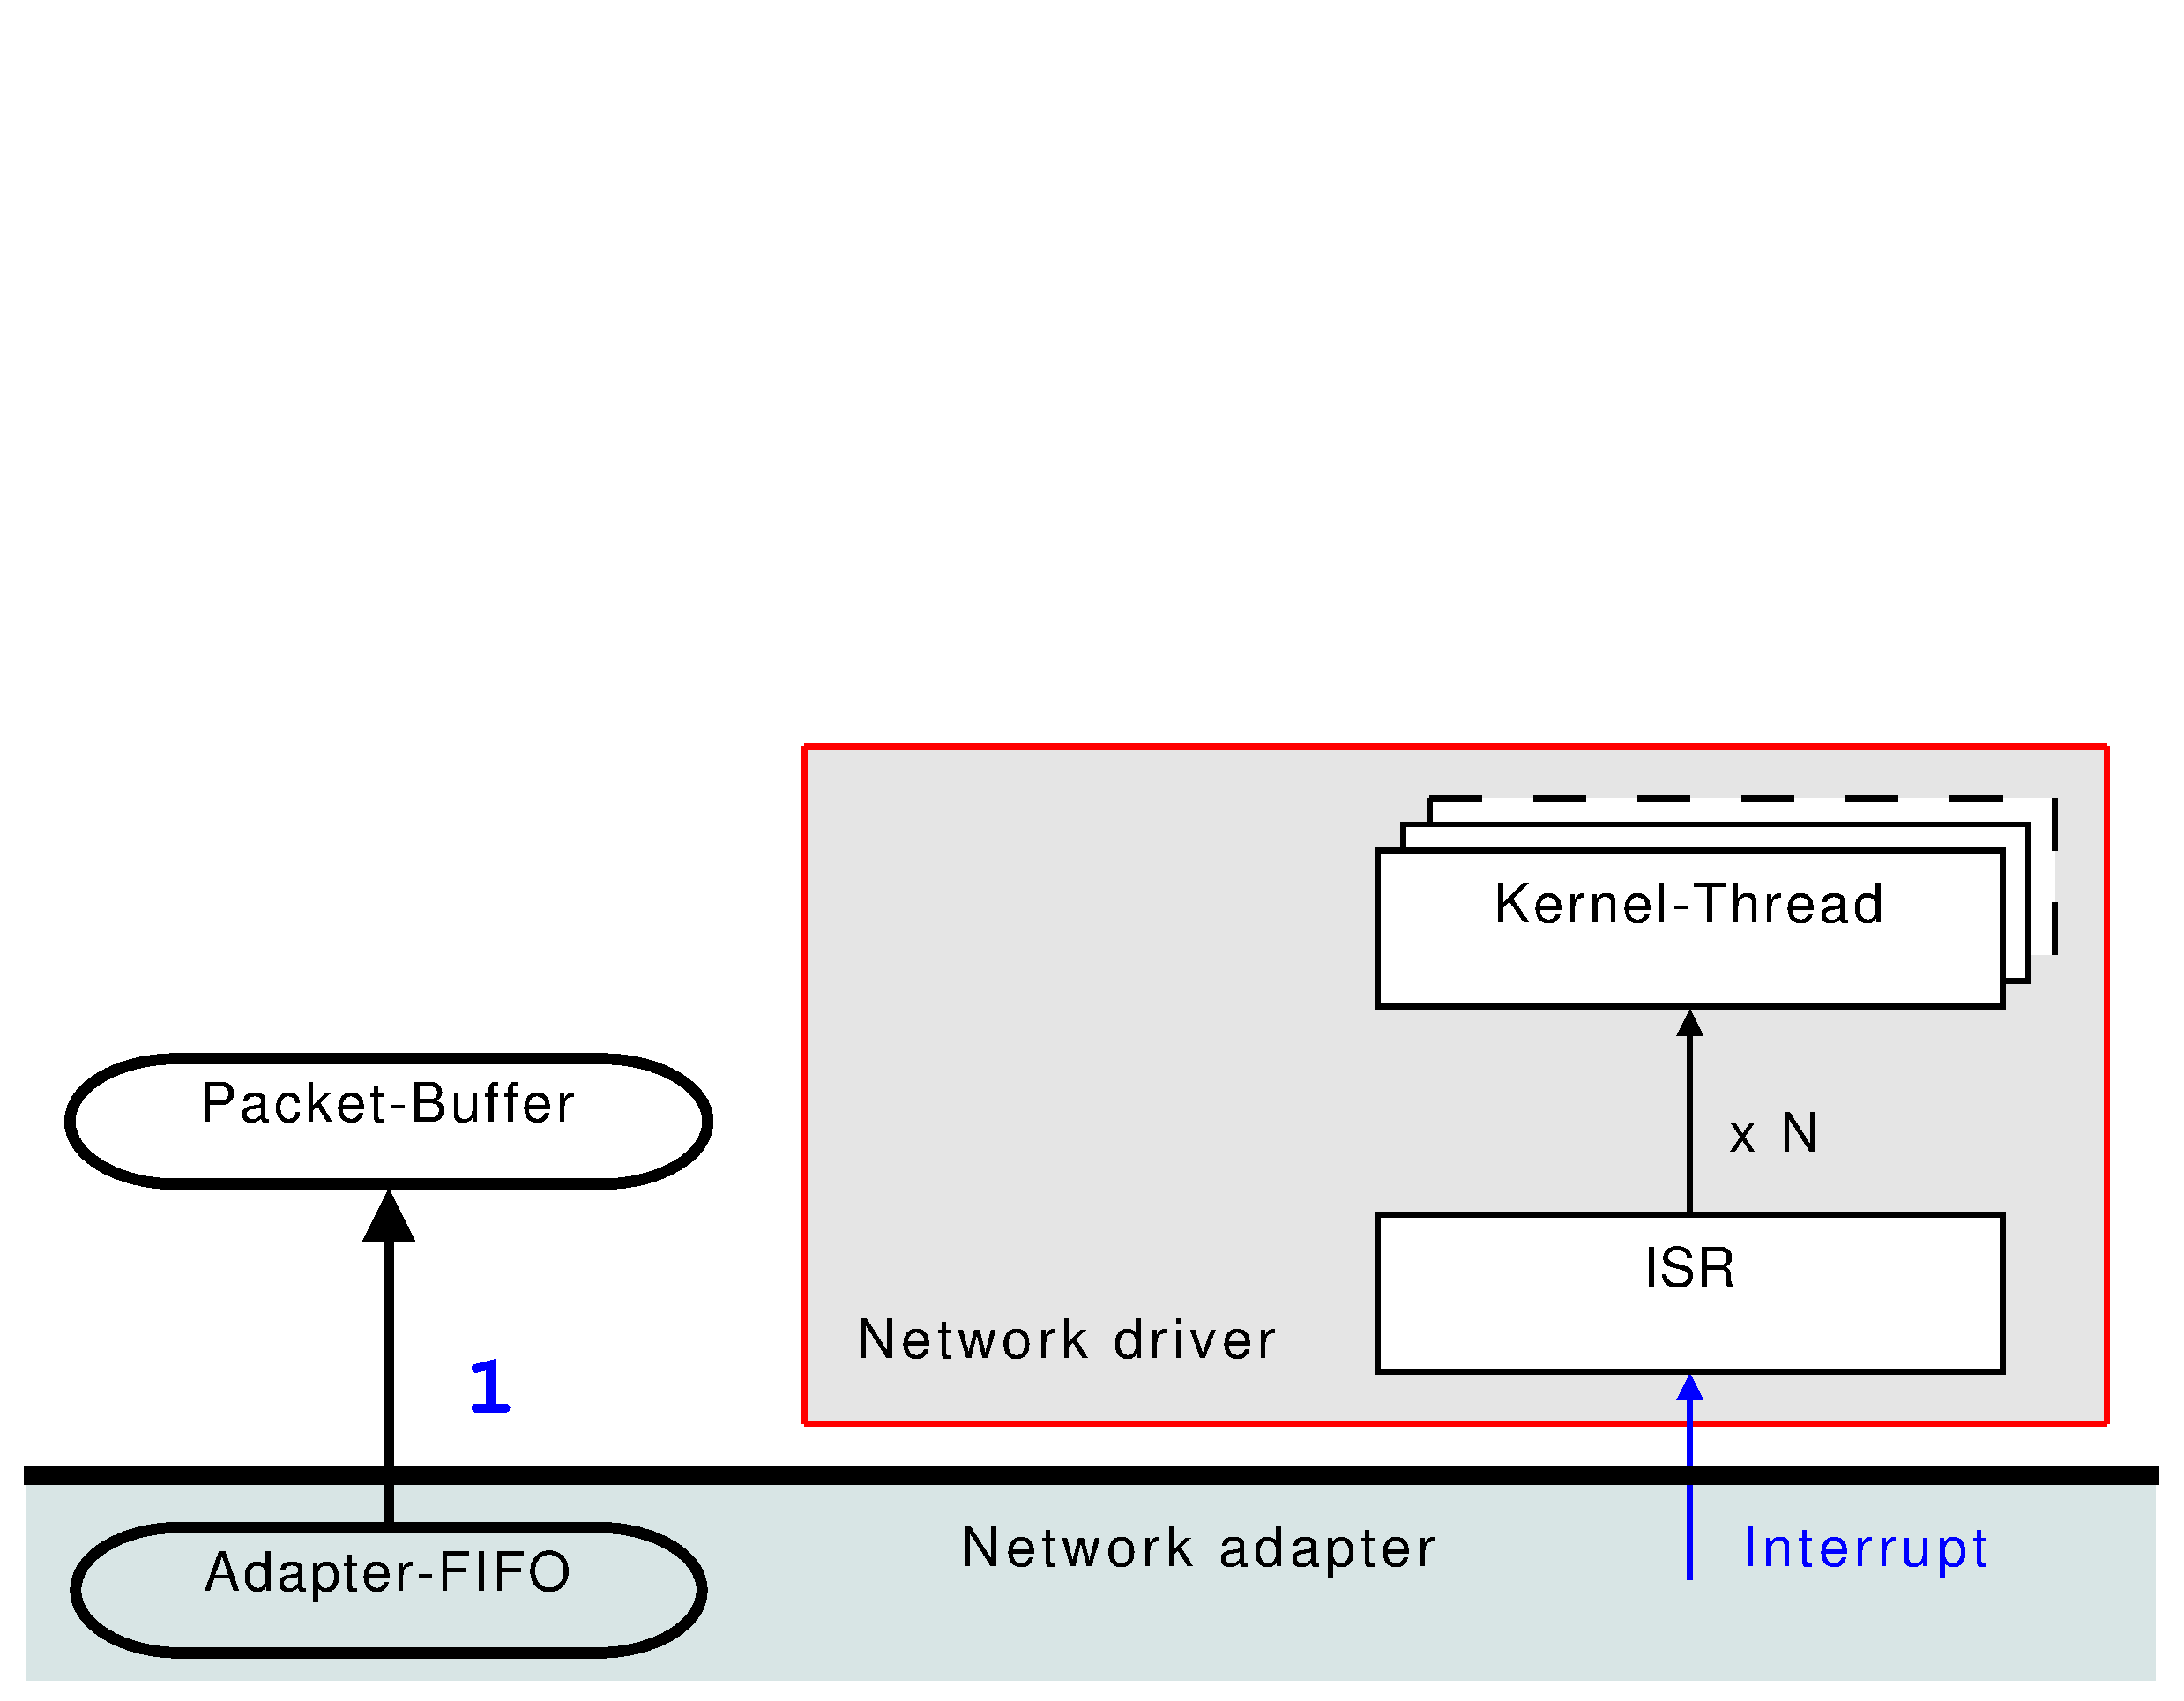
\includegraphics [height=55mm,width=60mm]{pics/3copy_1}}
%	\only<5>{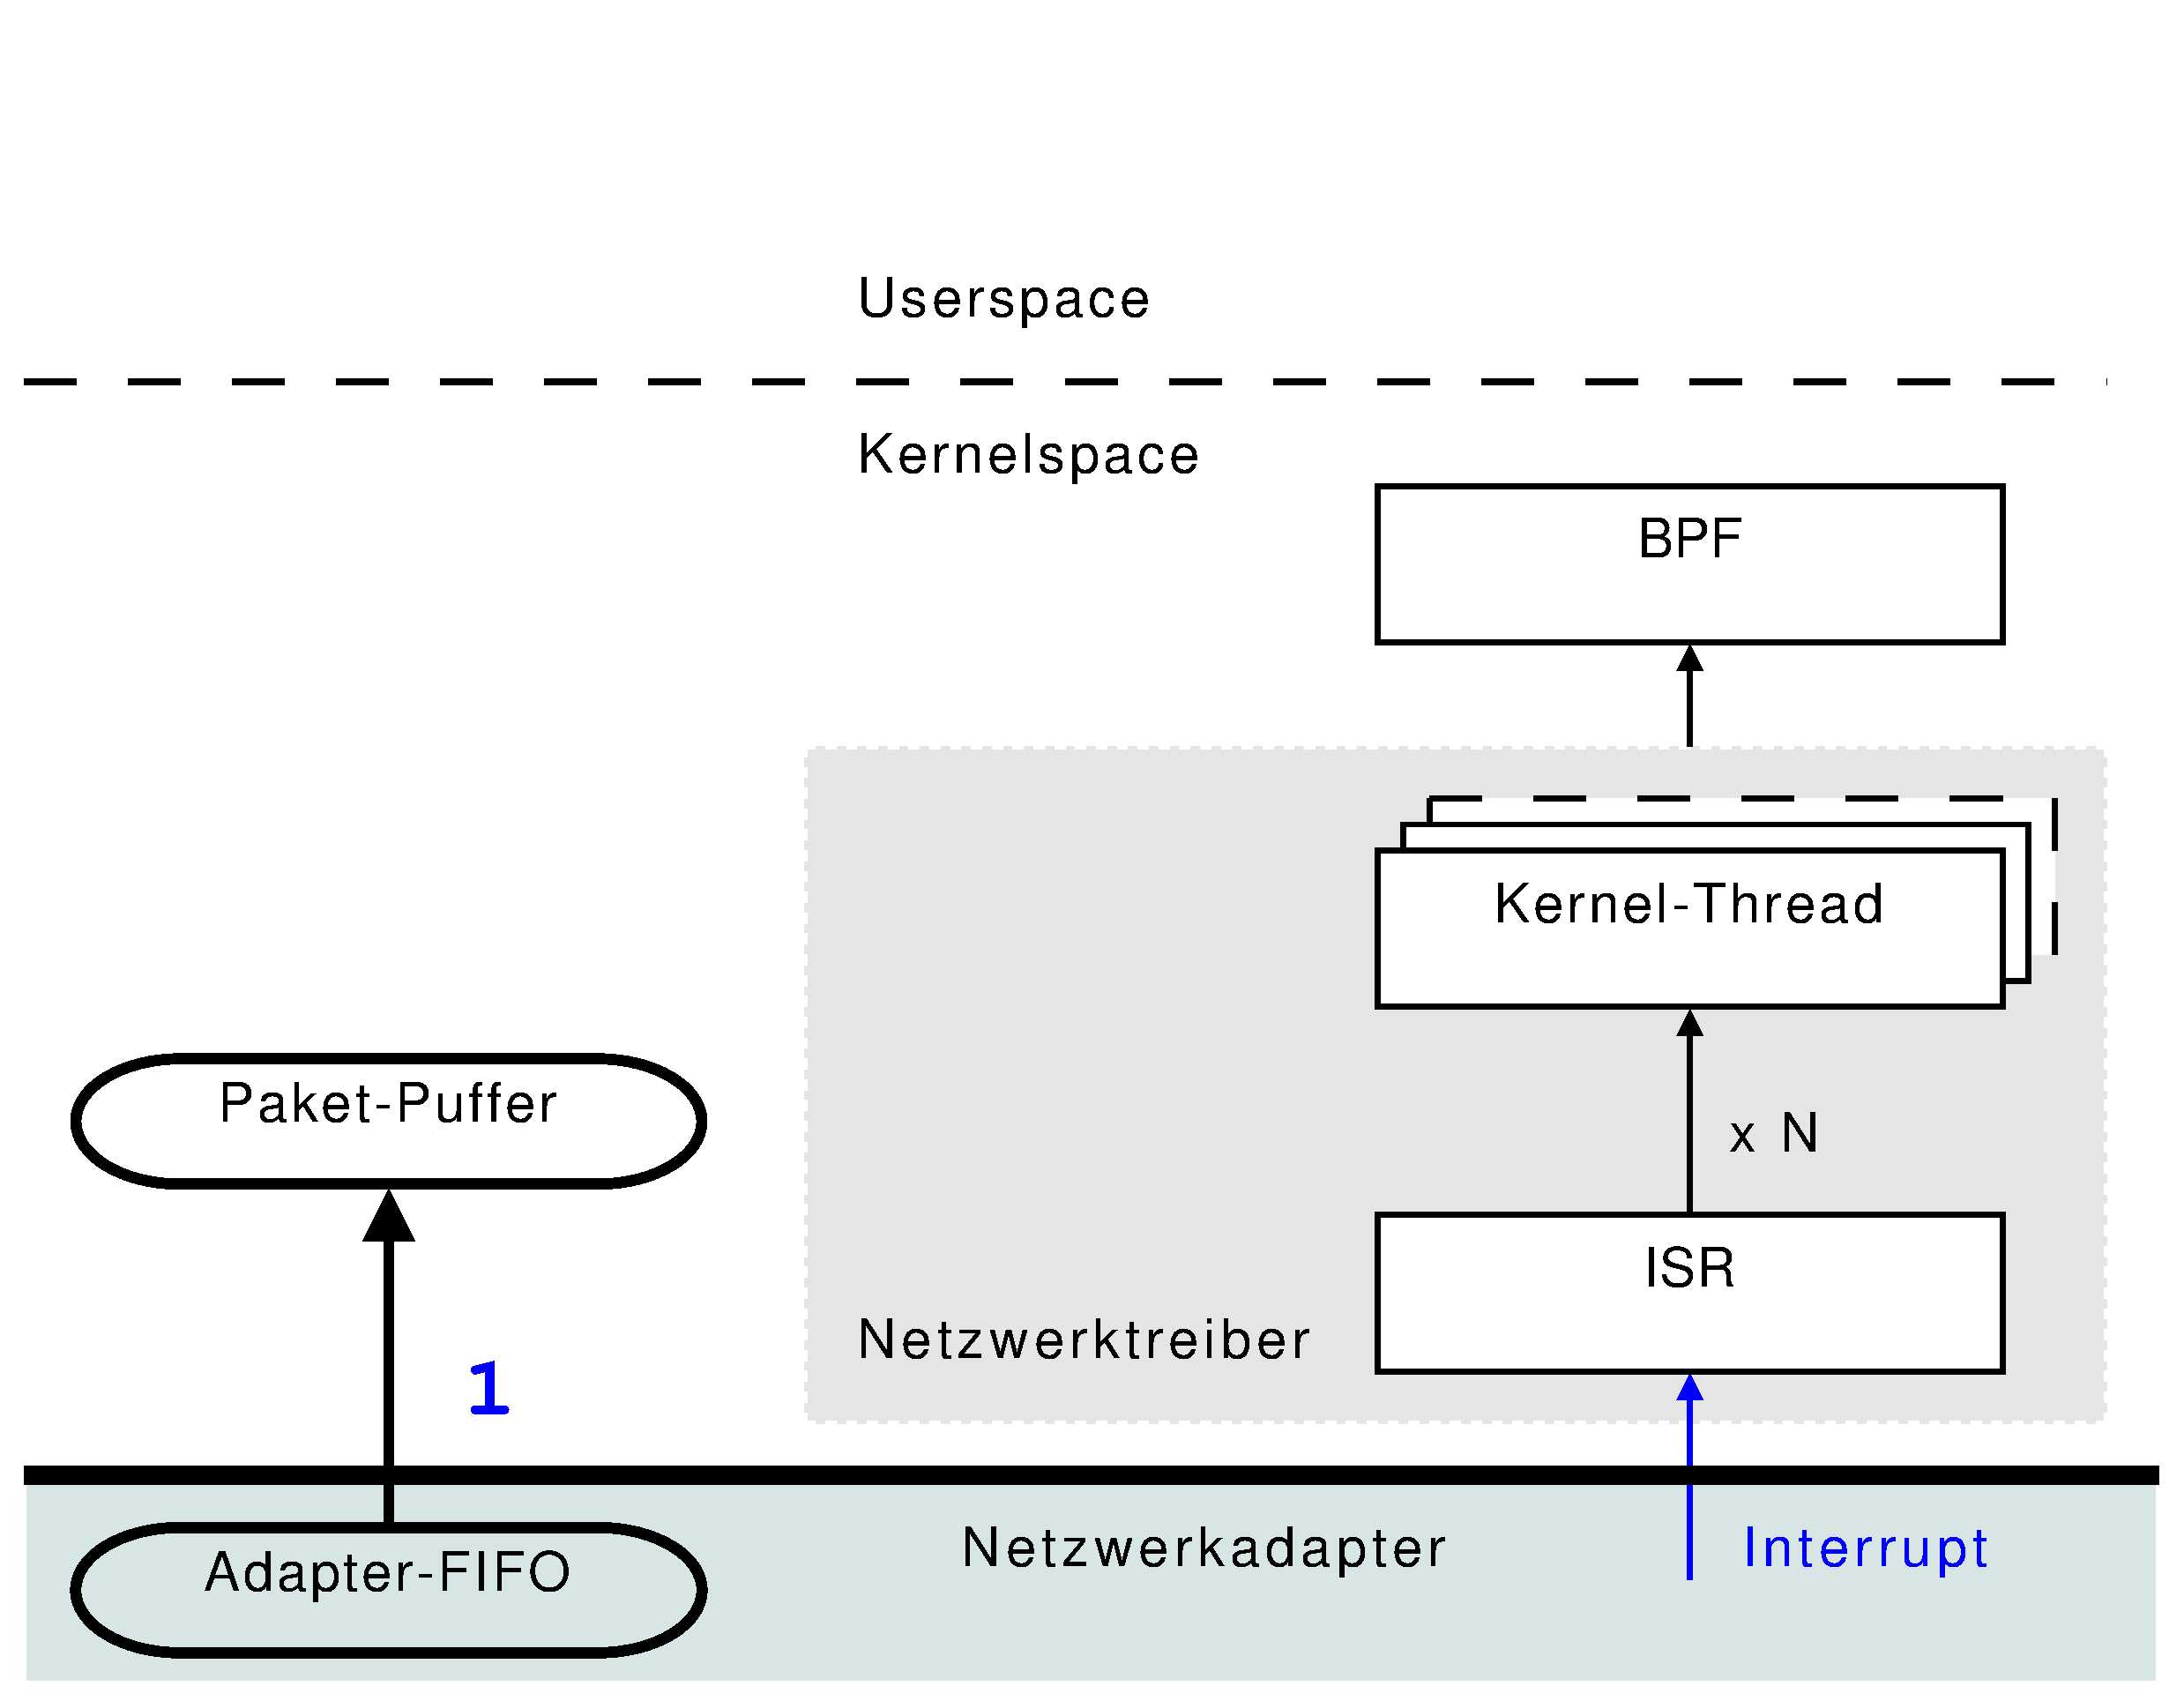
\includegraphics [height=55mm,width=60mm]{pics/3copy_1_1}}
	\only<5>{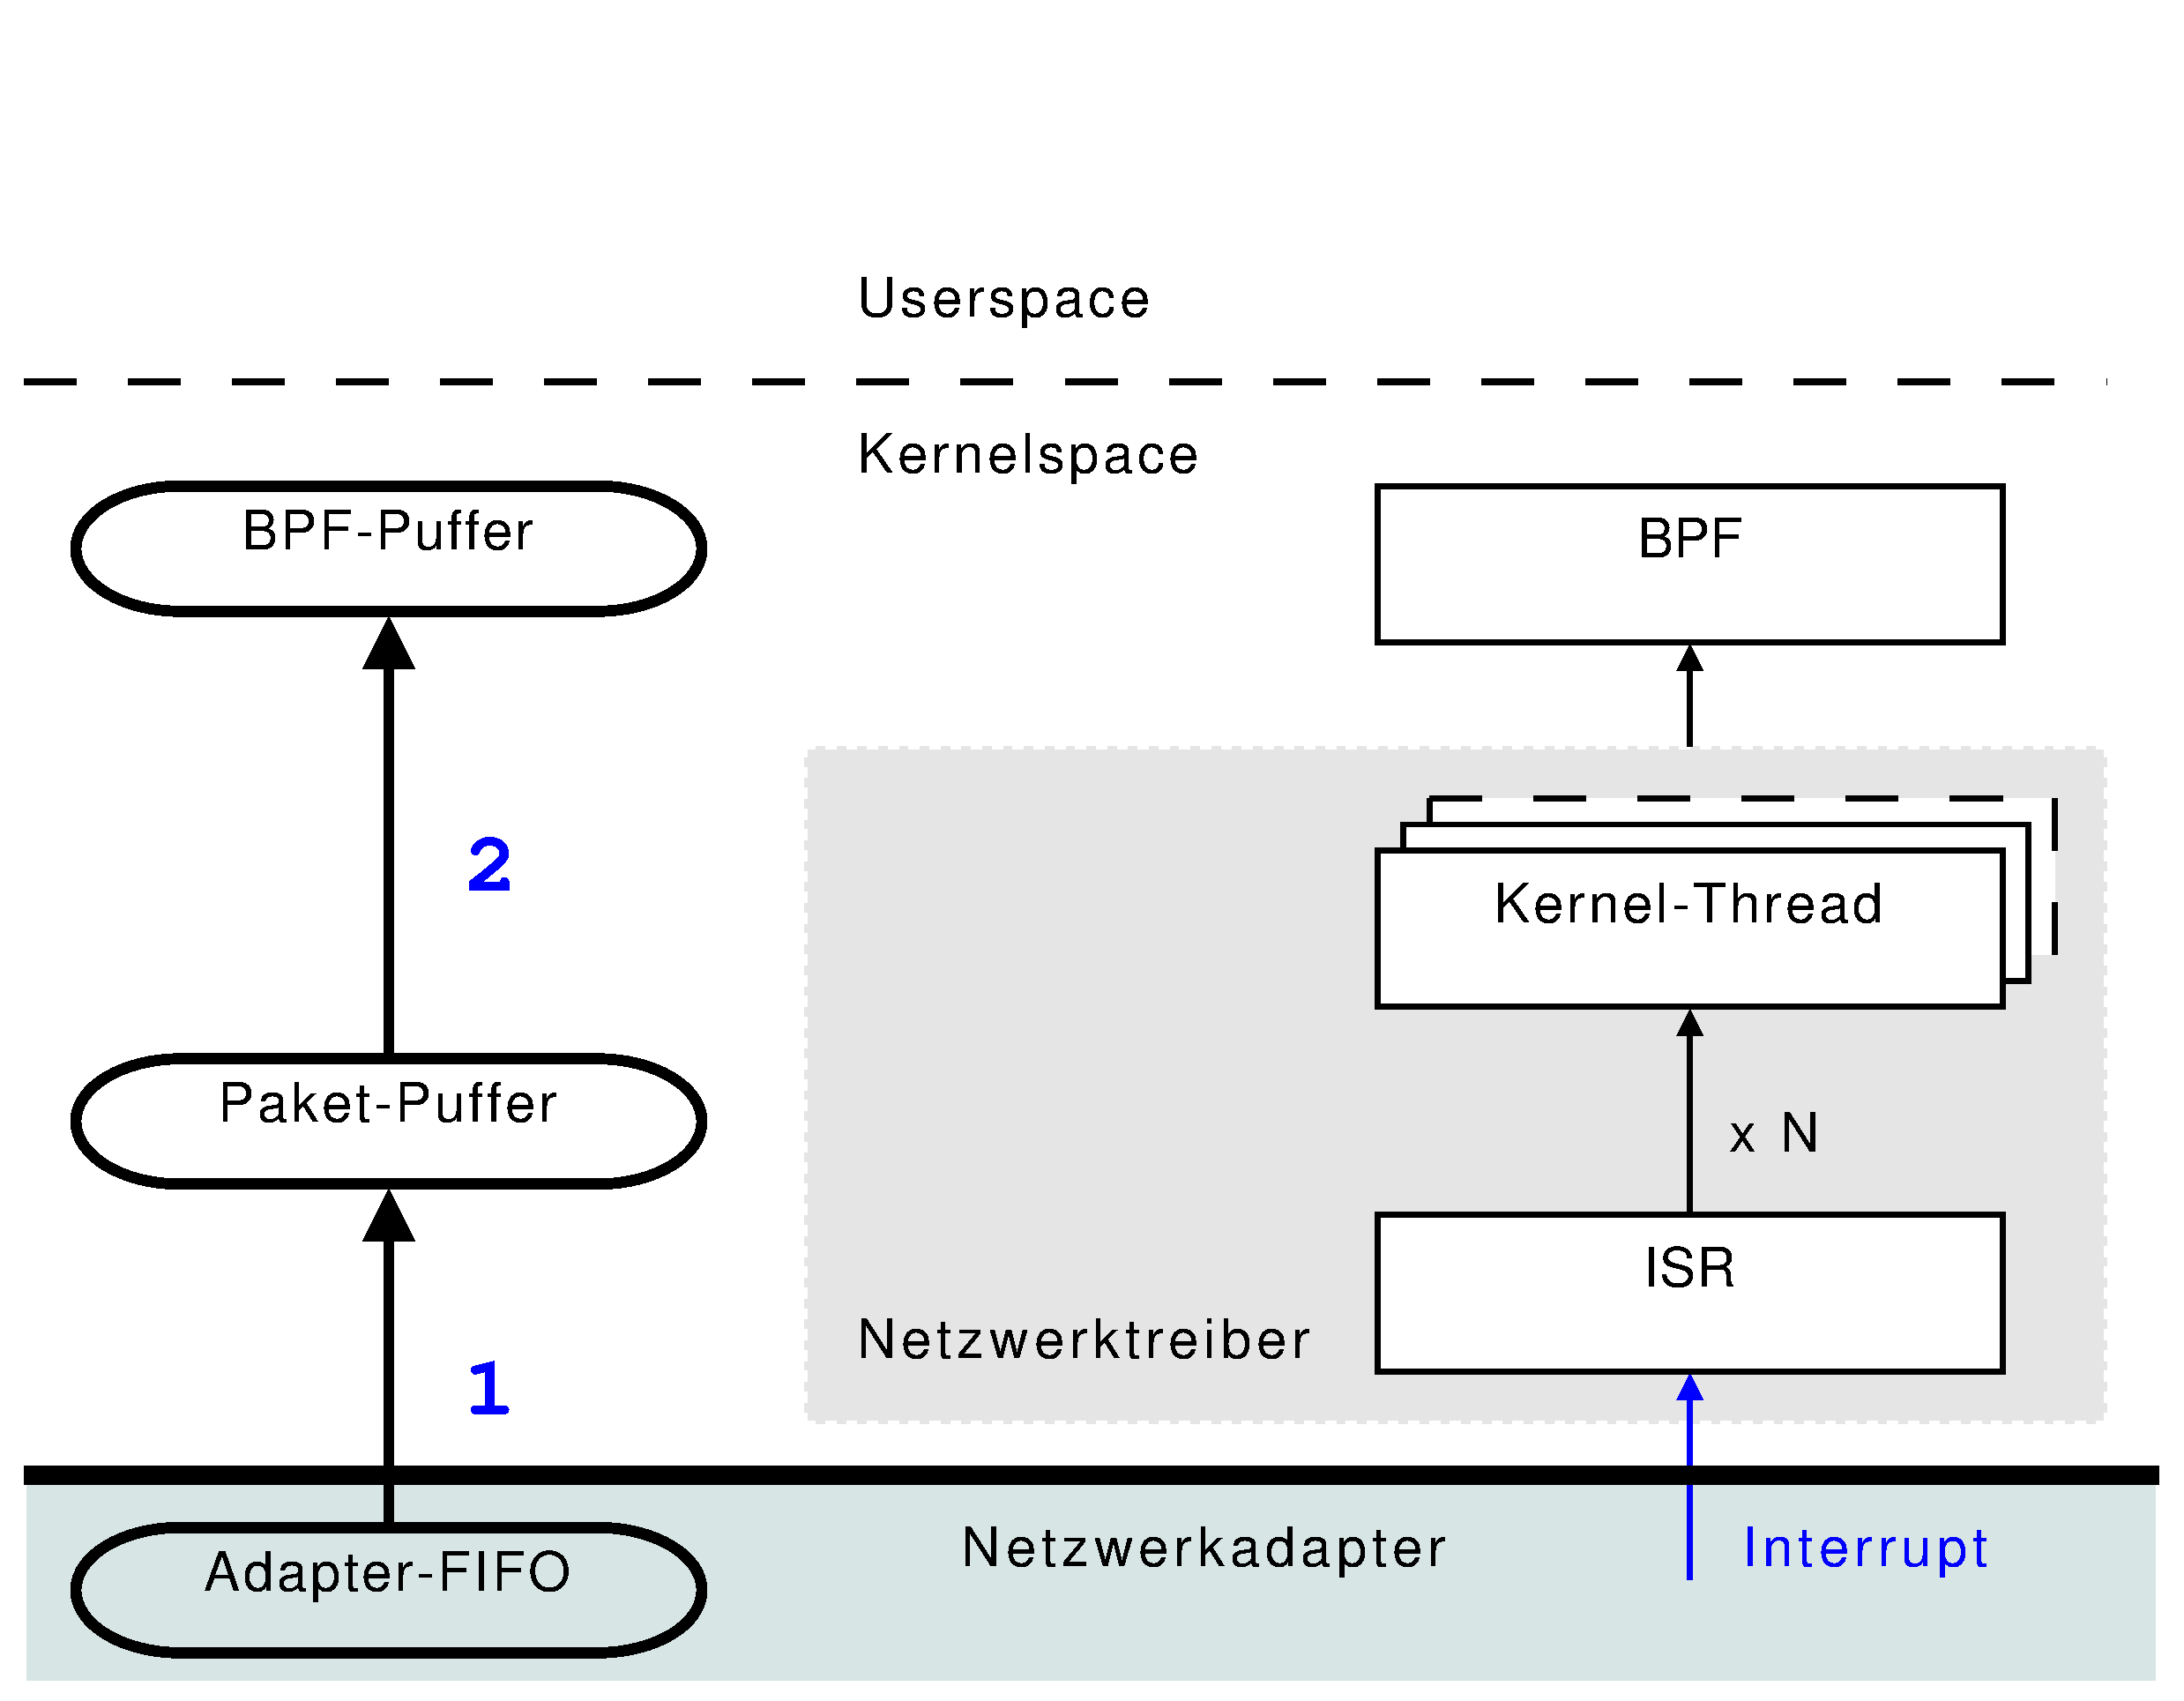
\includegraphics [height=55mm,width=60mm]{pics/3copy_2}}
	\only<6>{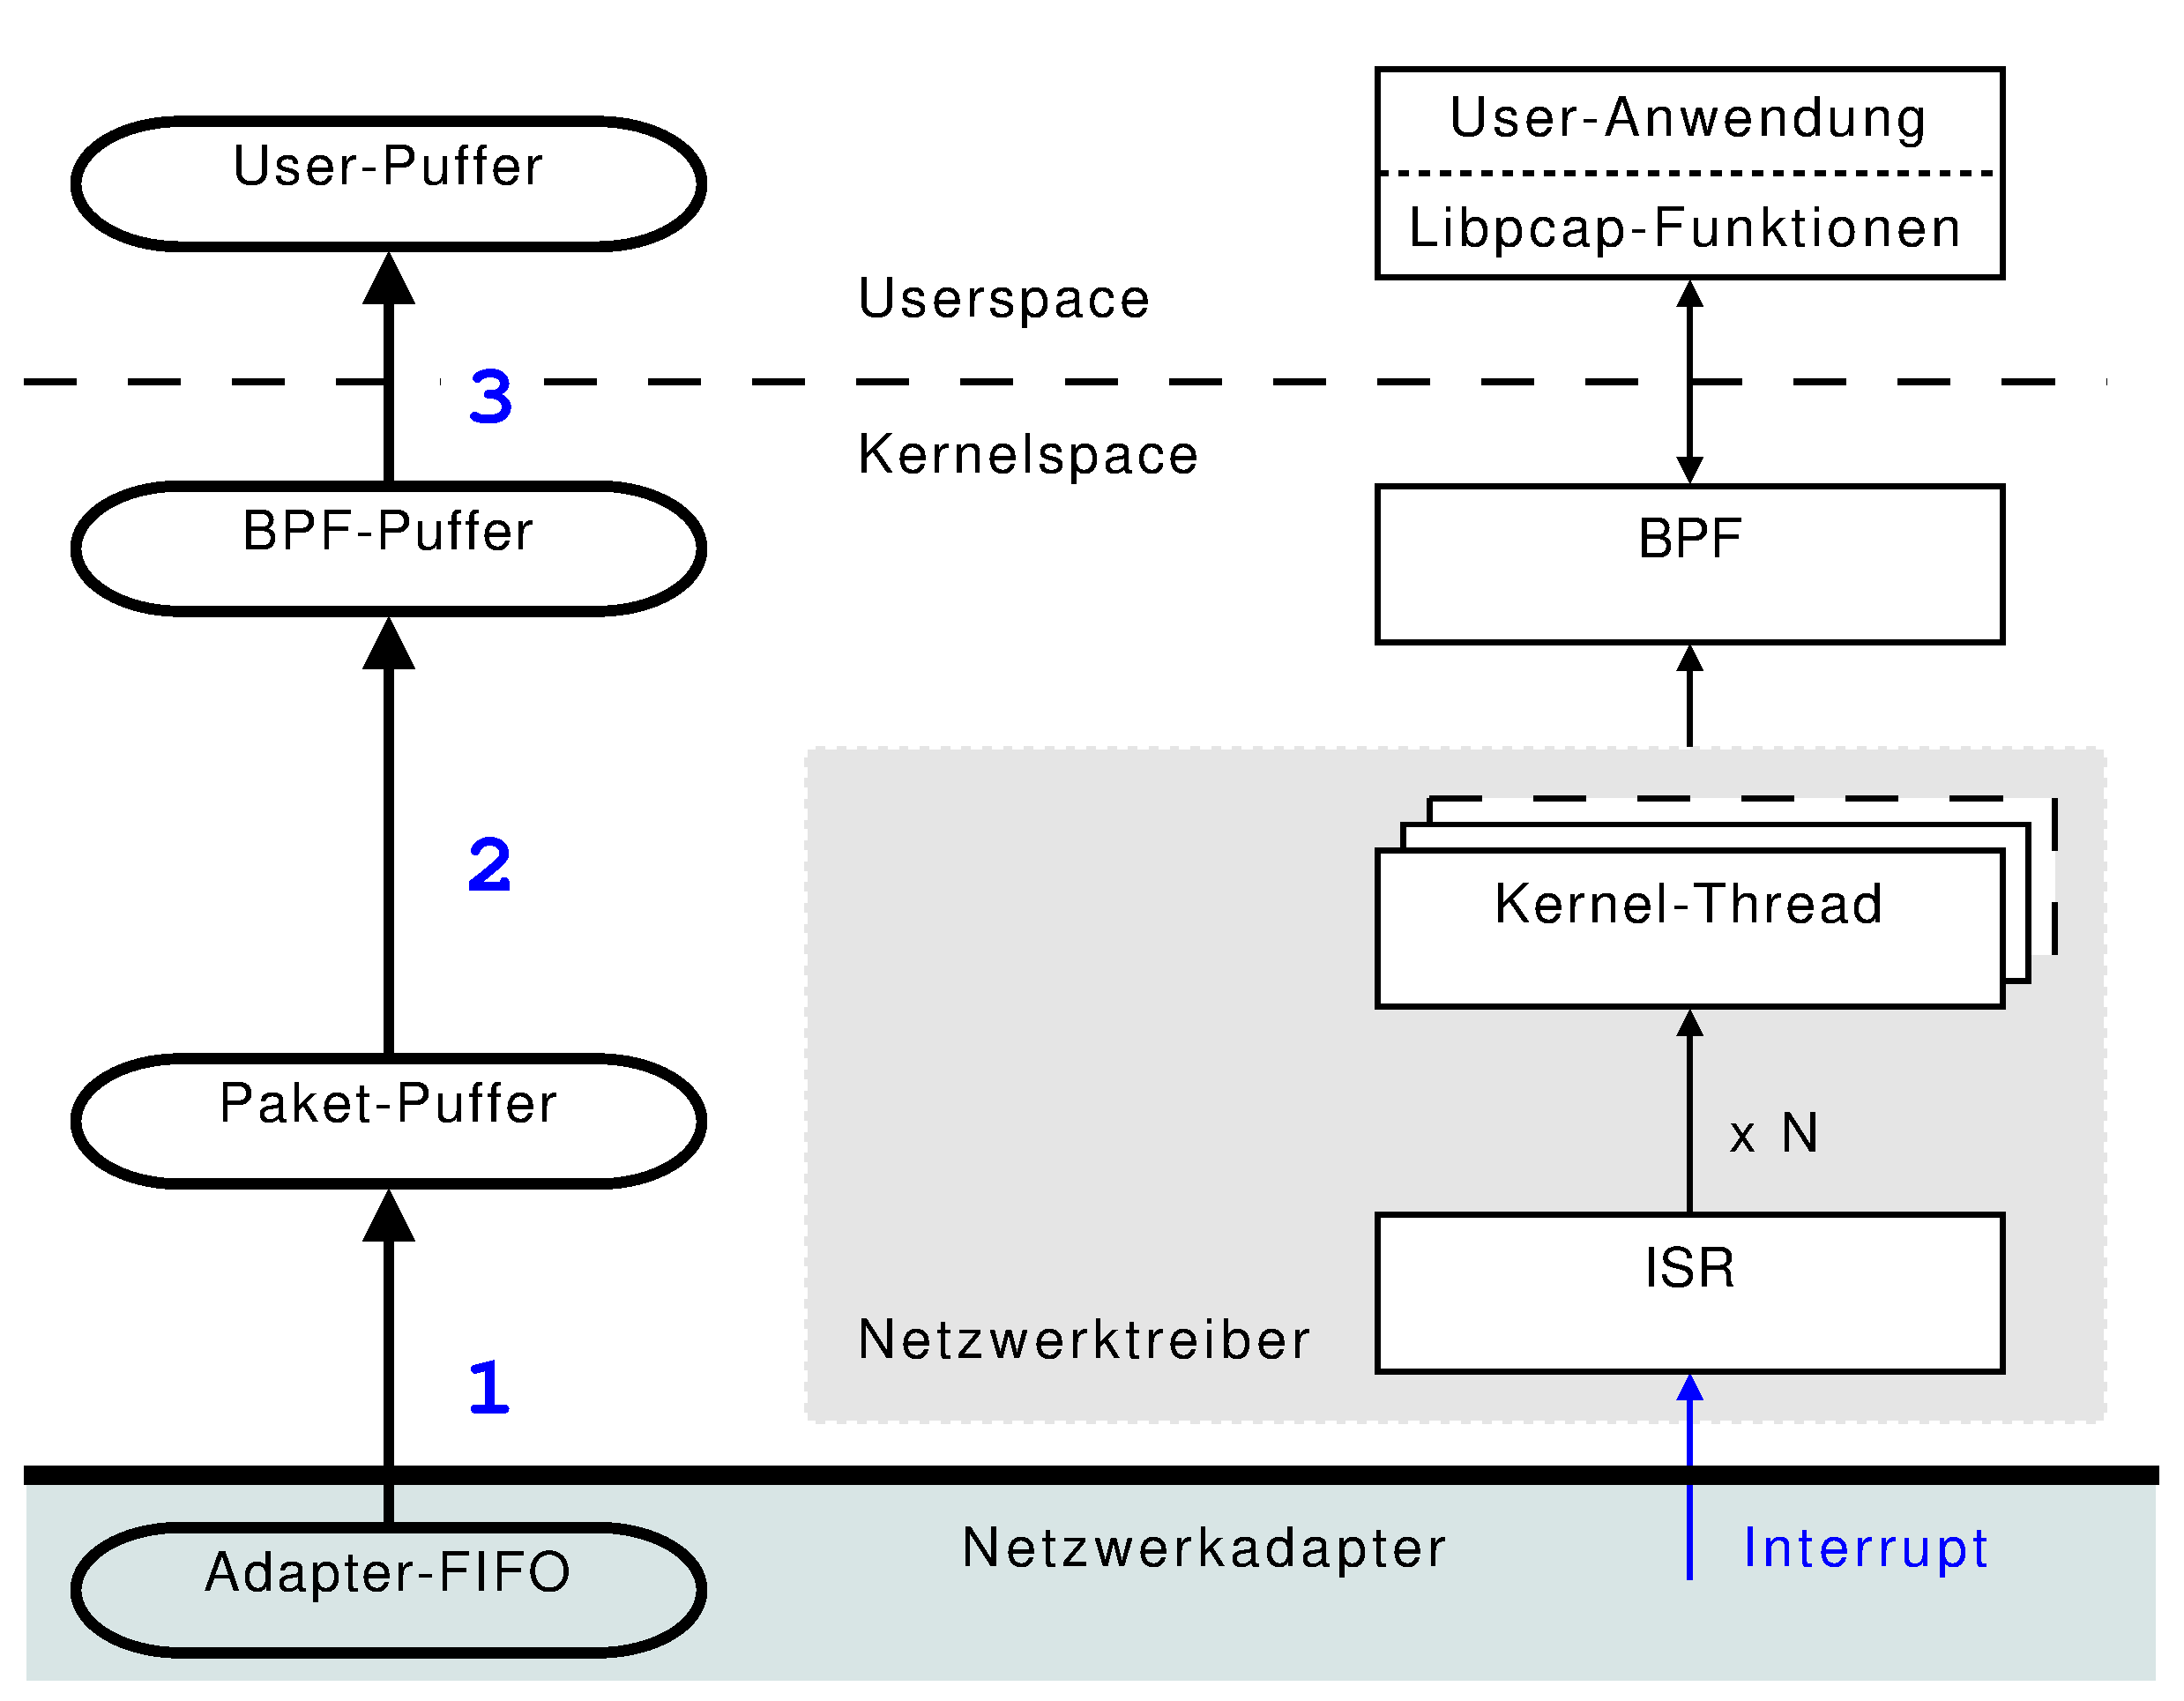
\includegraphics [height=55mm,width=60mm]{pics/3copy_3}}
\end{figure}
\end{columns}
\end{frame}

%%%%%%%%%%%%%%%%%%%%%%%%%%%%%%%%%%%%%%%%%%%%%%%%%%%%%%%%%%%%%%%%%%%
\begin{frame}
\frametitle{Disadvantages of Standard Packet Capturing Stack}
\begin{itemize}
	\item \textbf{Three copies per packet}
		\begin{enumerate}
			\item DMA: $FIFO \Rightarrow Packet\ Buffer$
			\item $Packet\ Buffer \Rightarrow BPF\ Buffer$
			\item $BPF\ Buffer \Rightarrow Userspace\ Buffer$\emph{(*)}
		\end{enumerate}
	\item \textbf{Memory allocations }
		\begin{itemize}
			\item For each new received packet will be a new \emph{mbuf} 
				allocated
		\end{itemize}
	\item \textbf{System calls }
		\begin{itemize}
			\item User-space application receives the packets using read(2)\emph{(*)}
			\item Saving packets to the hard disk
		\end{itemize}
\end{itemize}
\begin{tiny}
\emph{(*)} Using Zero-Copy BPF eliminates the last copy and system call
\end{tiny}
\end{frame}
%%%%%%%%%%%%%%%%%%%%%%%%%%%%%%%%%%%%%%%%%%%%%%%%%%%%%%%%%%%%%%%%%%%

%	Description of Task, Goal
\section{Solution}

\begin{frame}
	\begin{center}
	\huge{Solution}
	\end{center}
\end{frame}


\subsection*{Capturing stacks}
%%%%%%%%%%%%%%%%%%%%%%%%%%%%%%%%%%%%%%%%%%%%%%%%%%%%%%%%%%%%%%%%%%%
\begin{frame}
\frametitle{Ringmap Packet Capturing Stack}
\begin{itemize}
	\item \textbf{Ringmap}: The new packet capturing stack
	\item based on standard FreeBSD packet capturing stack: 		
		\begin{itemize}
			\item based on generic network drivers and \emph{libpcap}
			\begin{itemize}
				\item but slightly changed.\newline
			\end{itemize}
		\end{itemize}
\end{itemize}
\end{frame}


\subsection*{Changes in generic-Stack}
%%%%%%%%%%%%%%%%%%%%%%%%%%%%%%%%%%%%%%%%%%%%%%%%%%%%%%%%%%%%%%%%%%%
\begin{frame}
	\frametitle{What did we change in \emph{generic}}
\begin{columns}
\column[t]{0.5\textwidth}
\begin{itemize}
	\item <2->Disabled TCP/IP-Stack\newline
	\item <3->BPF is accessible in both kernel and user-space\newline
	\item <4->Network driver, and Libpcap is modified
		\begin{itemize}
			\item BPF is unchanged
		\end{itemize}
\end{itemize}
\column[t]{0.5\textwidth}
\vspace{-2em}
\only<1>{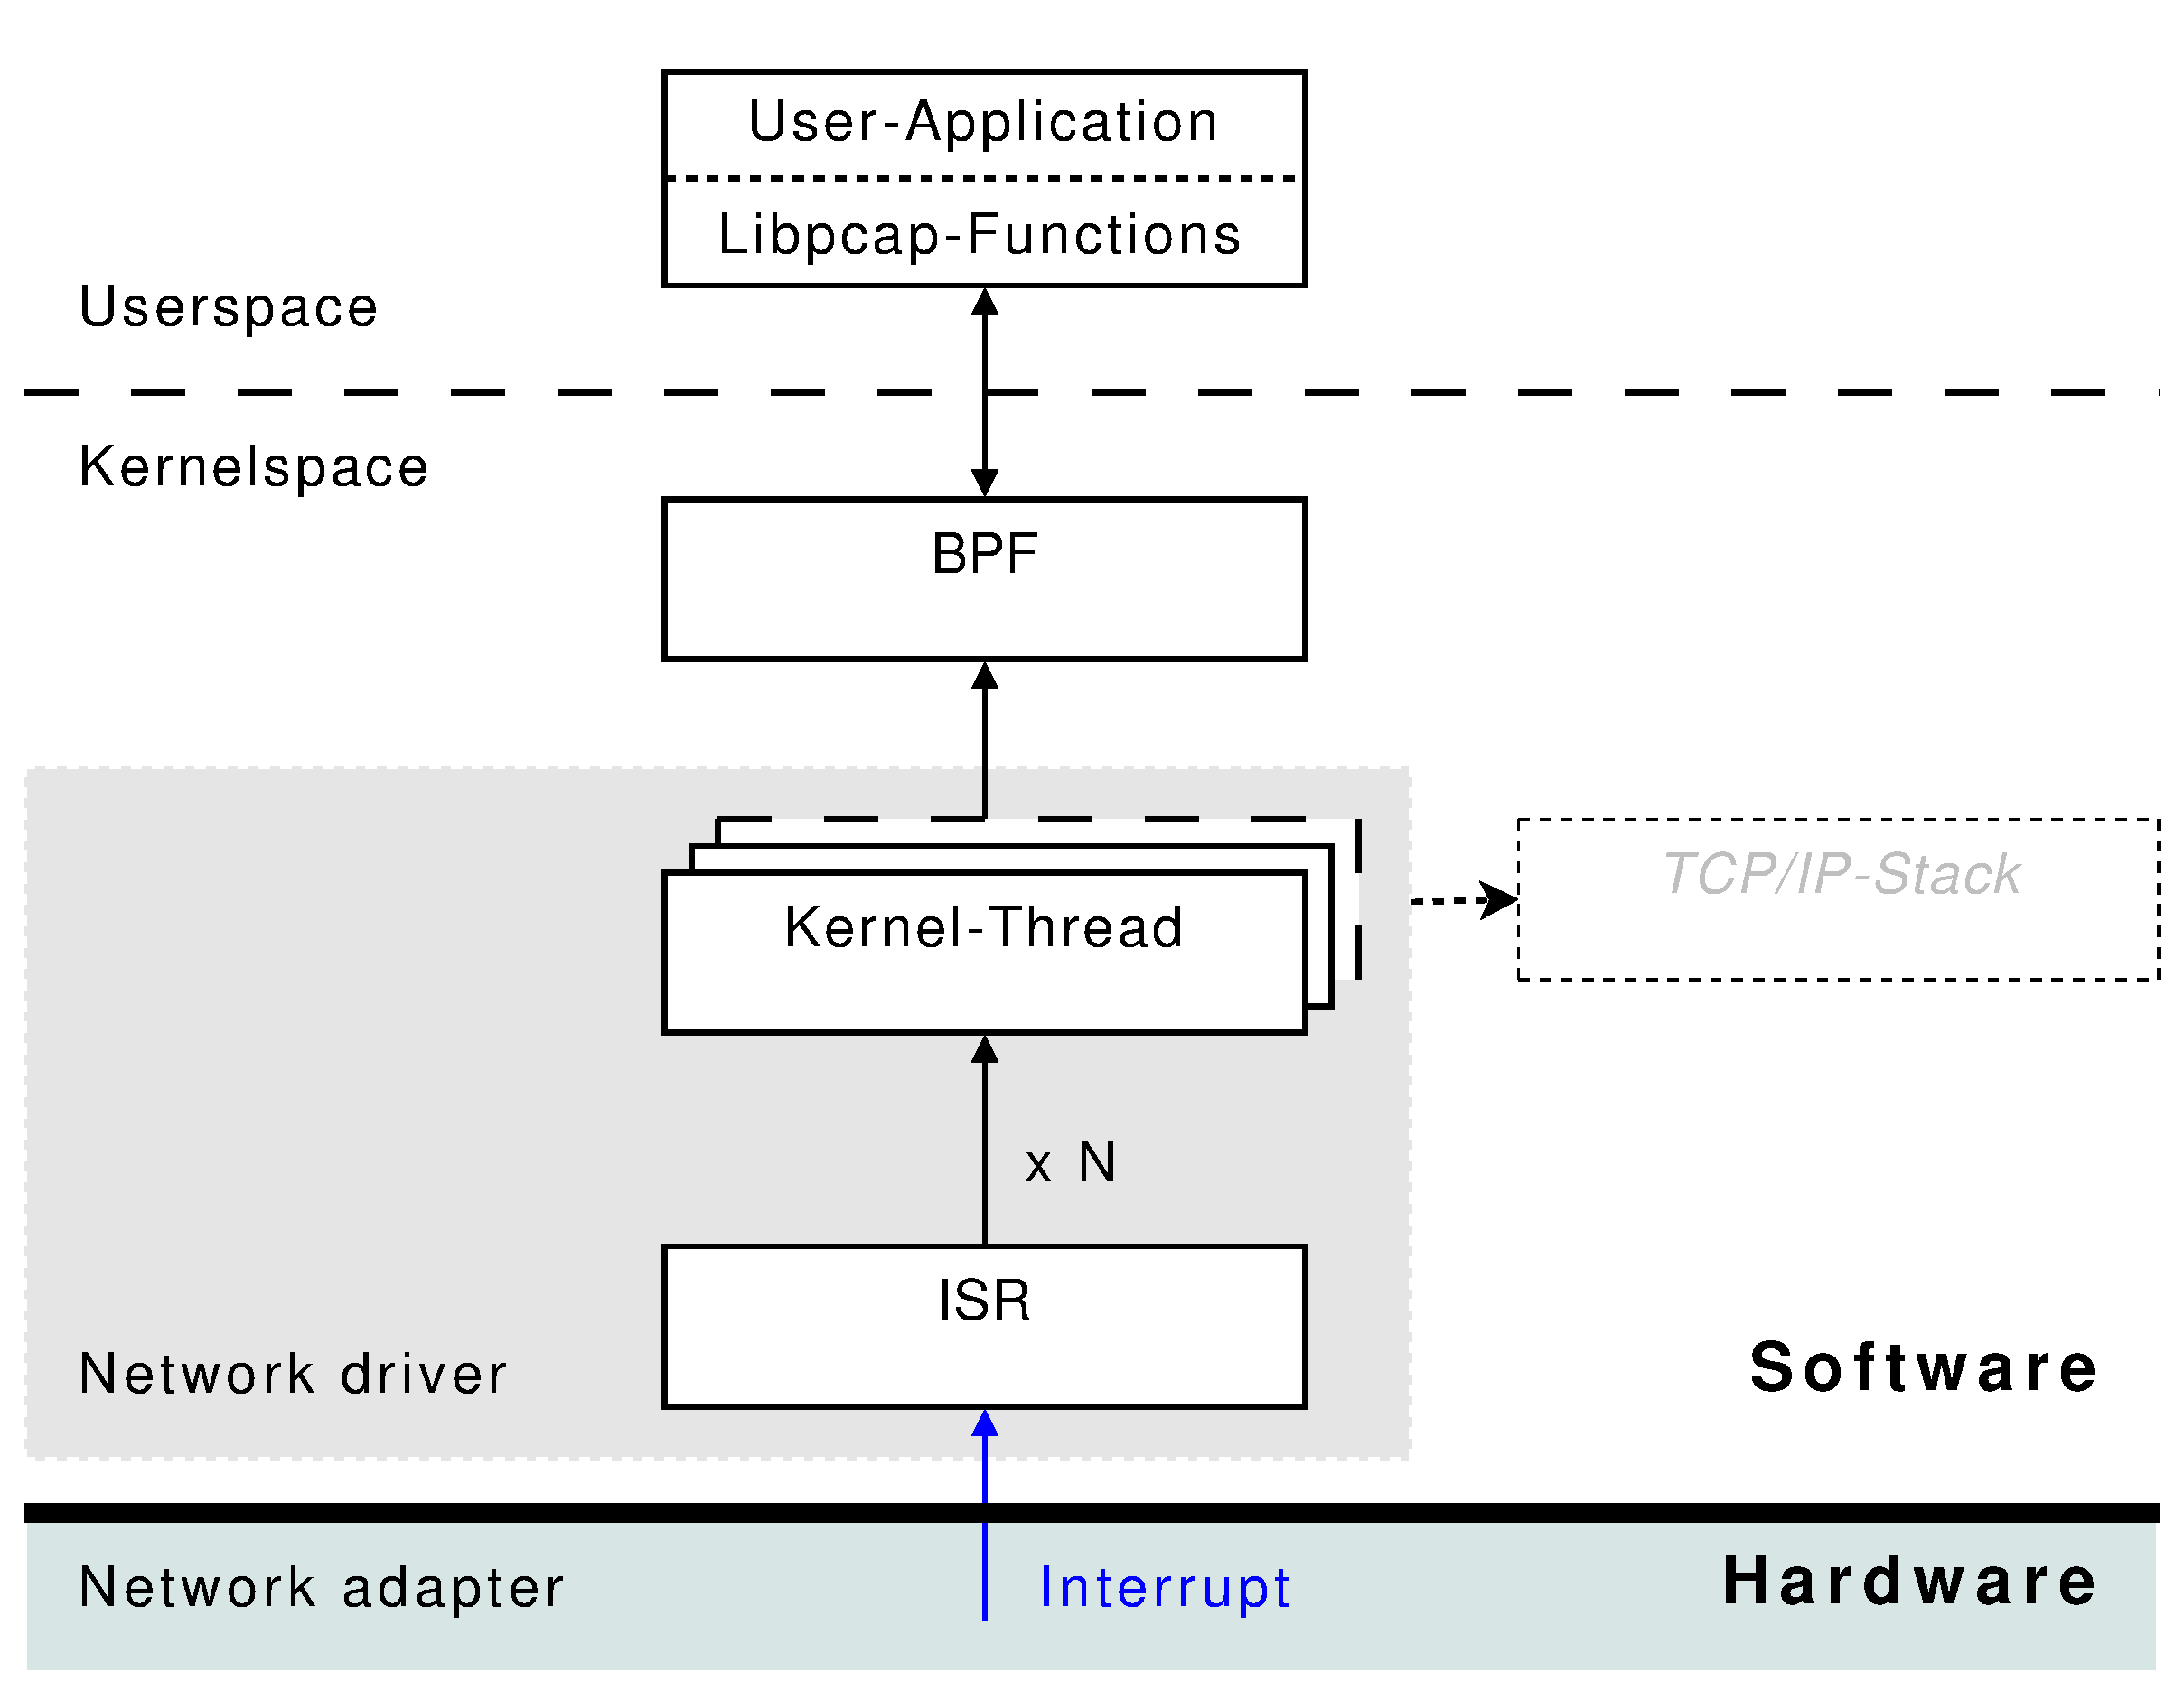
\includegraphics [height=55mm,width=60mm]{pics/PCS_funcs_ziel_DA_0}}
\only<2>{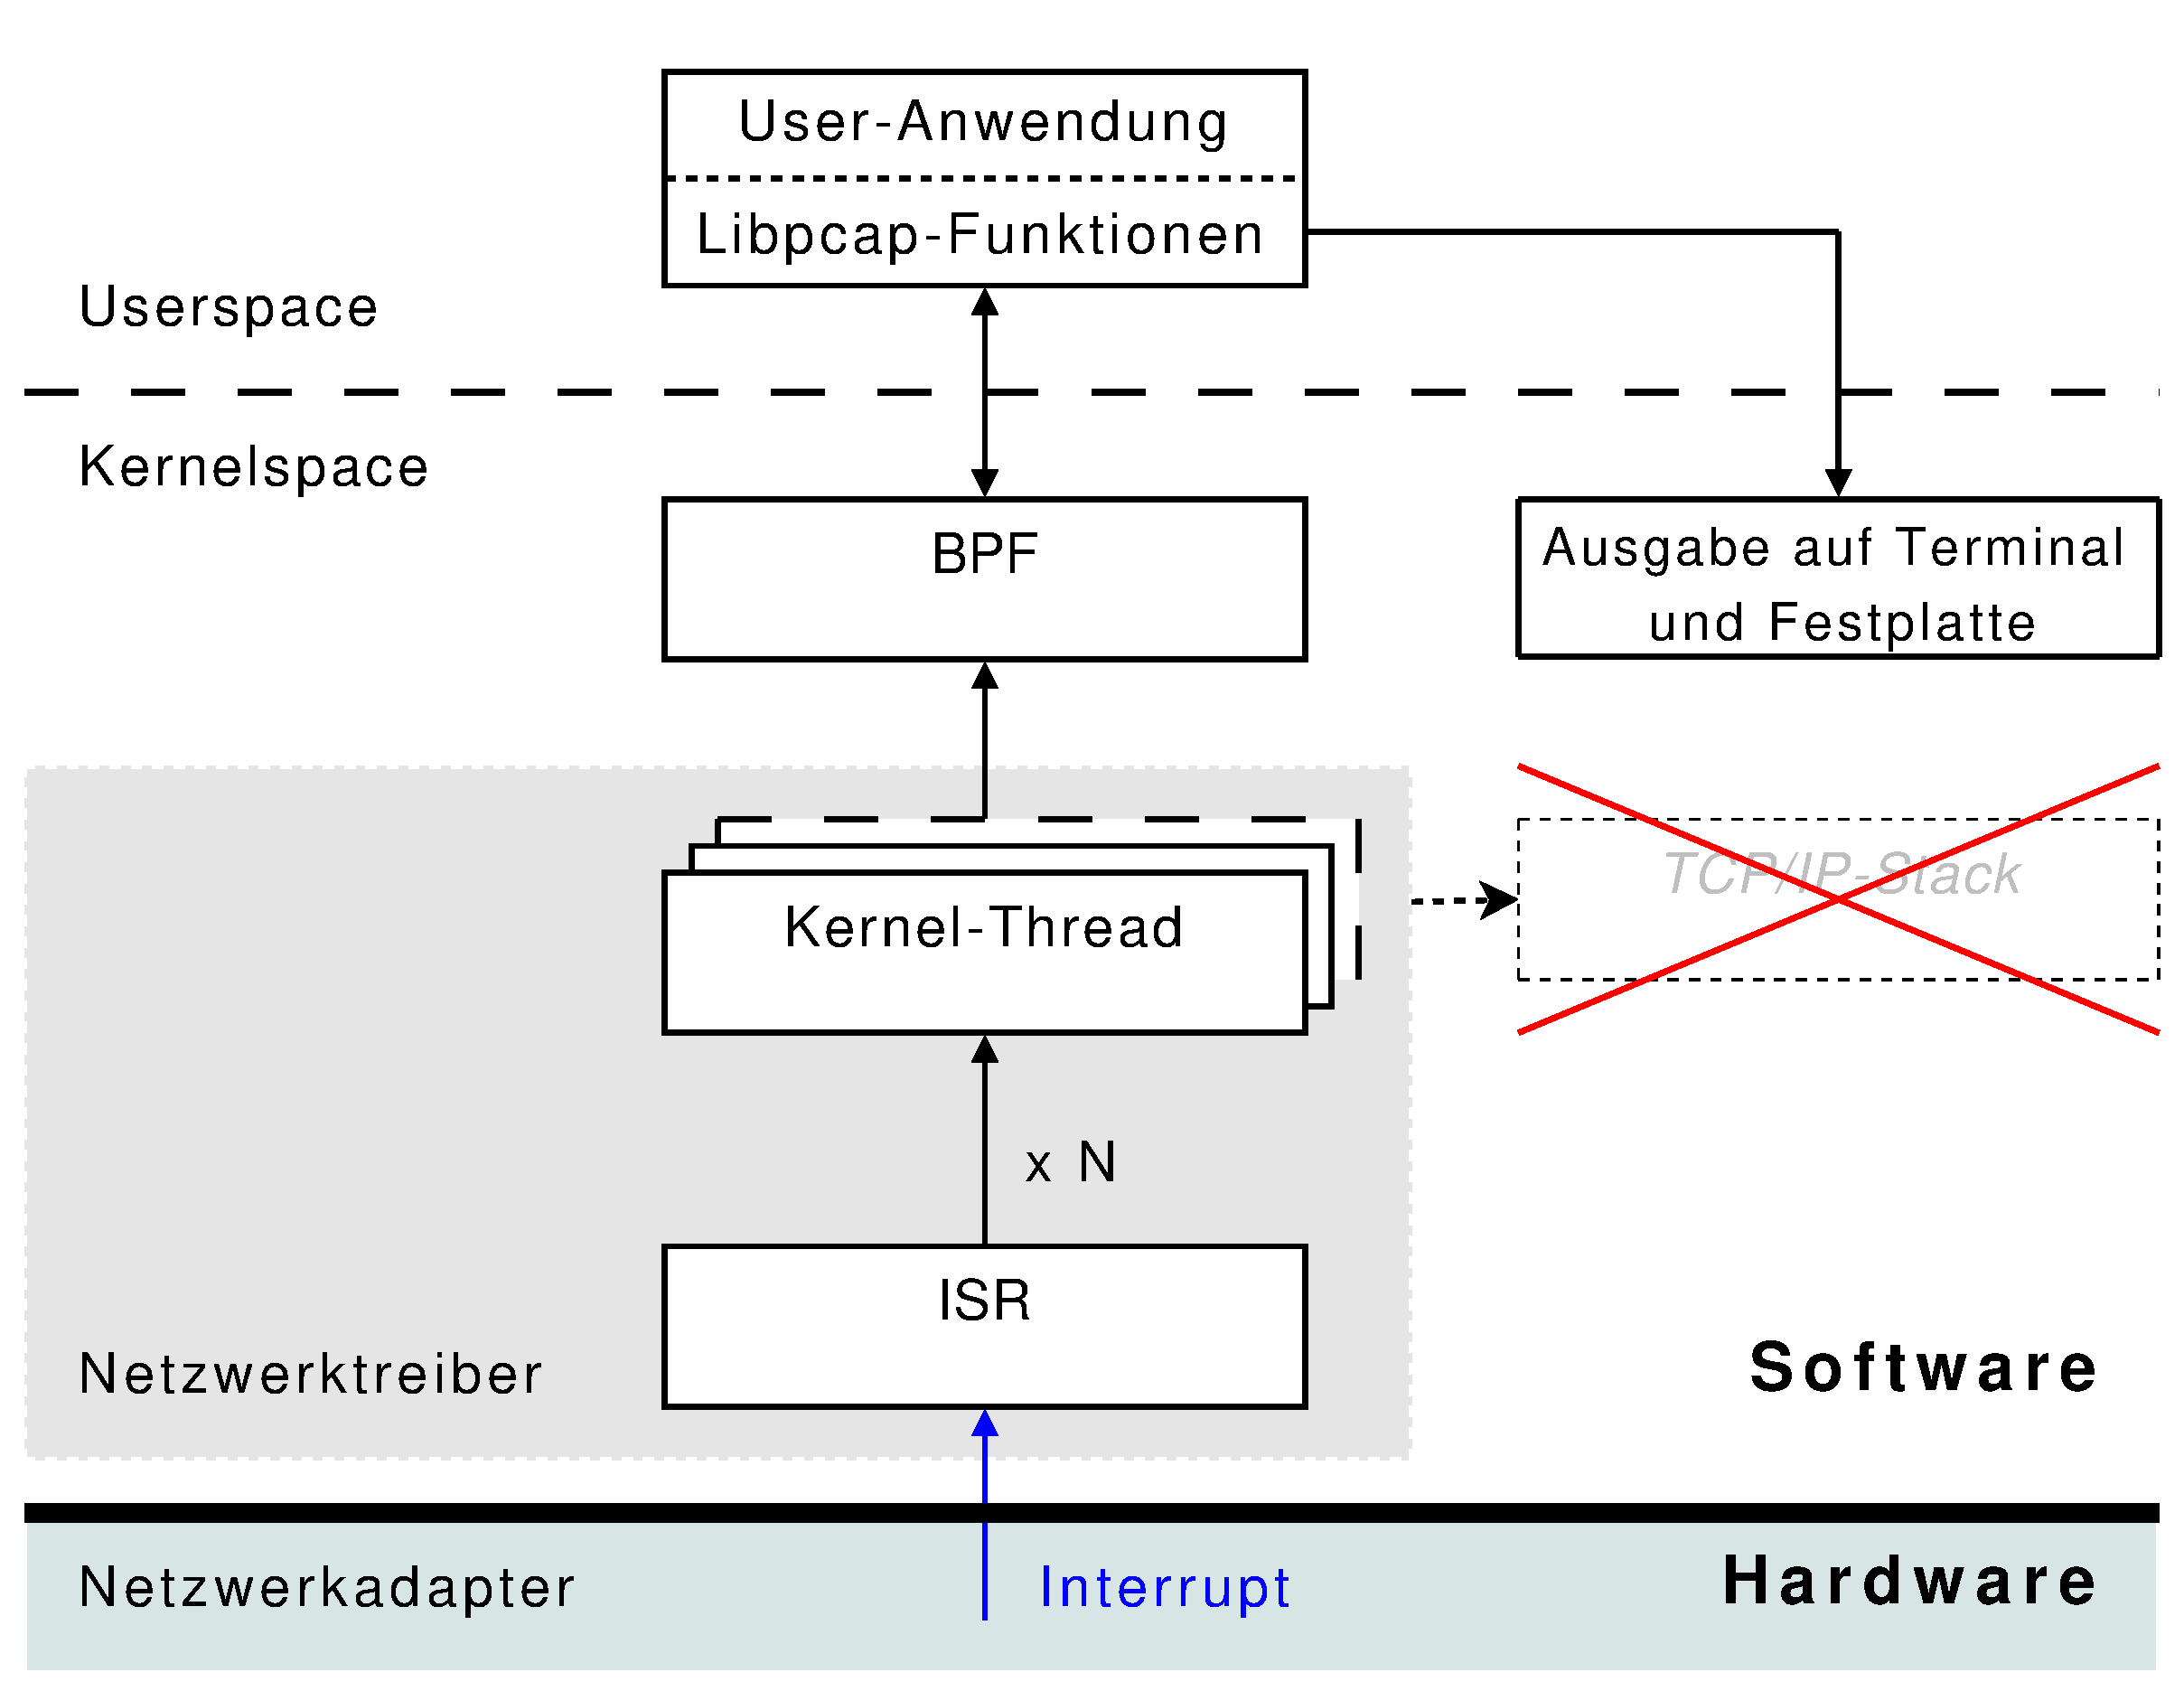
\includegraphics [height=55mm,width=60mm]{pics/PCS_funcs_ziel_DA_1}}
\only<3>{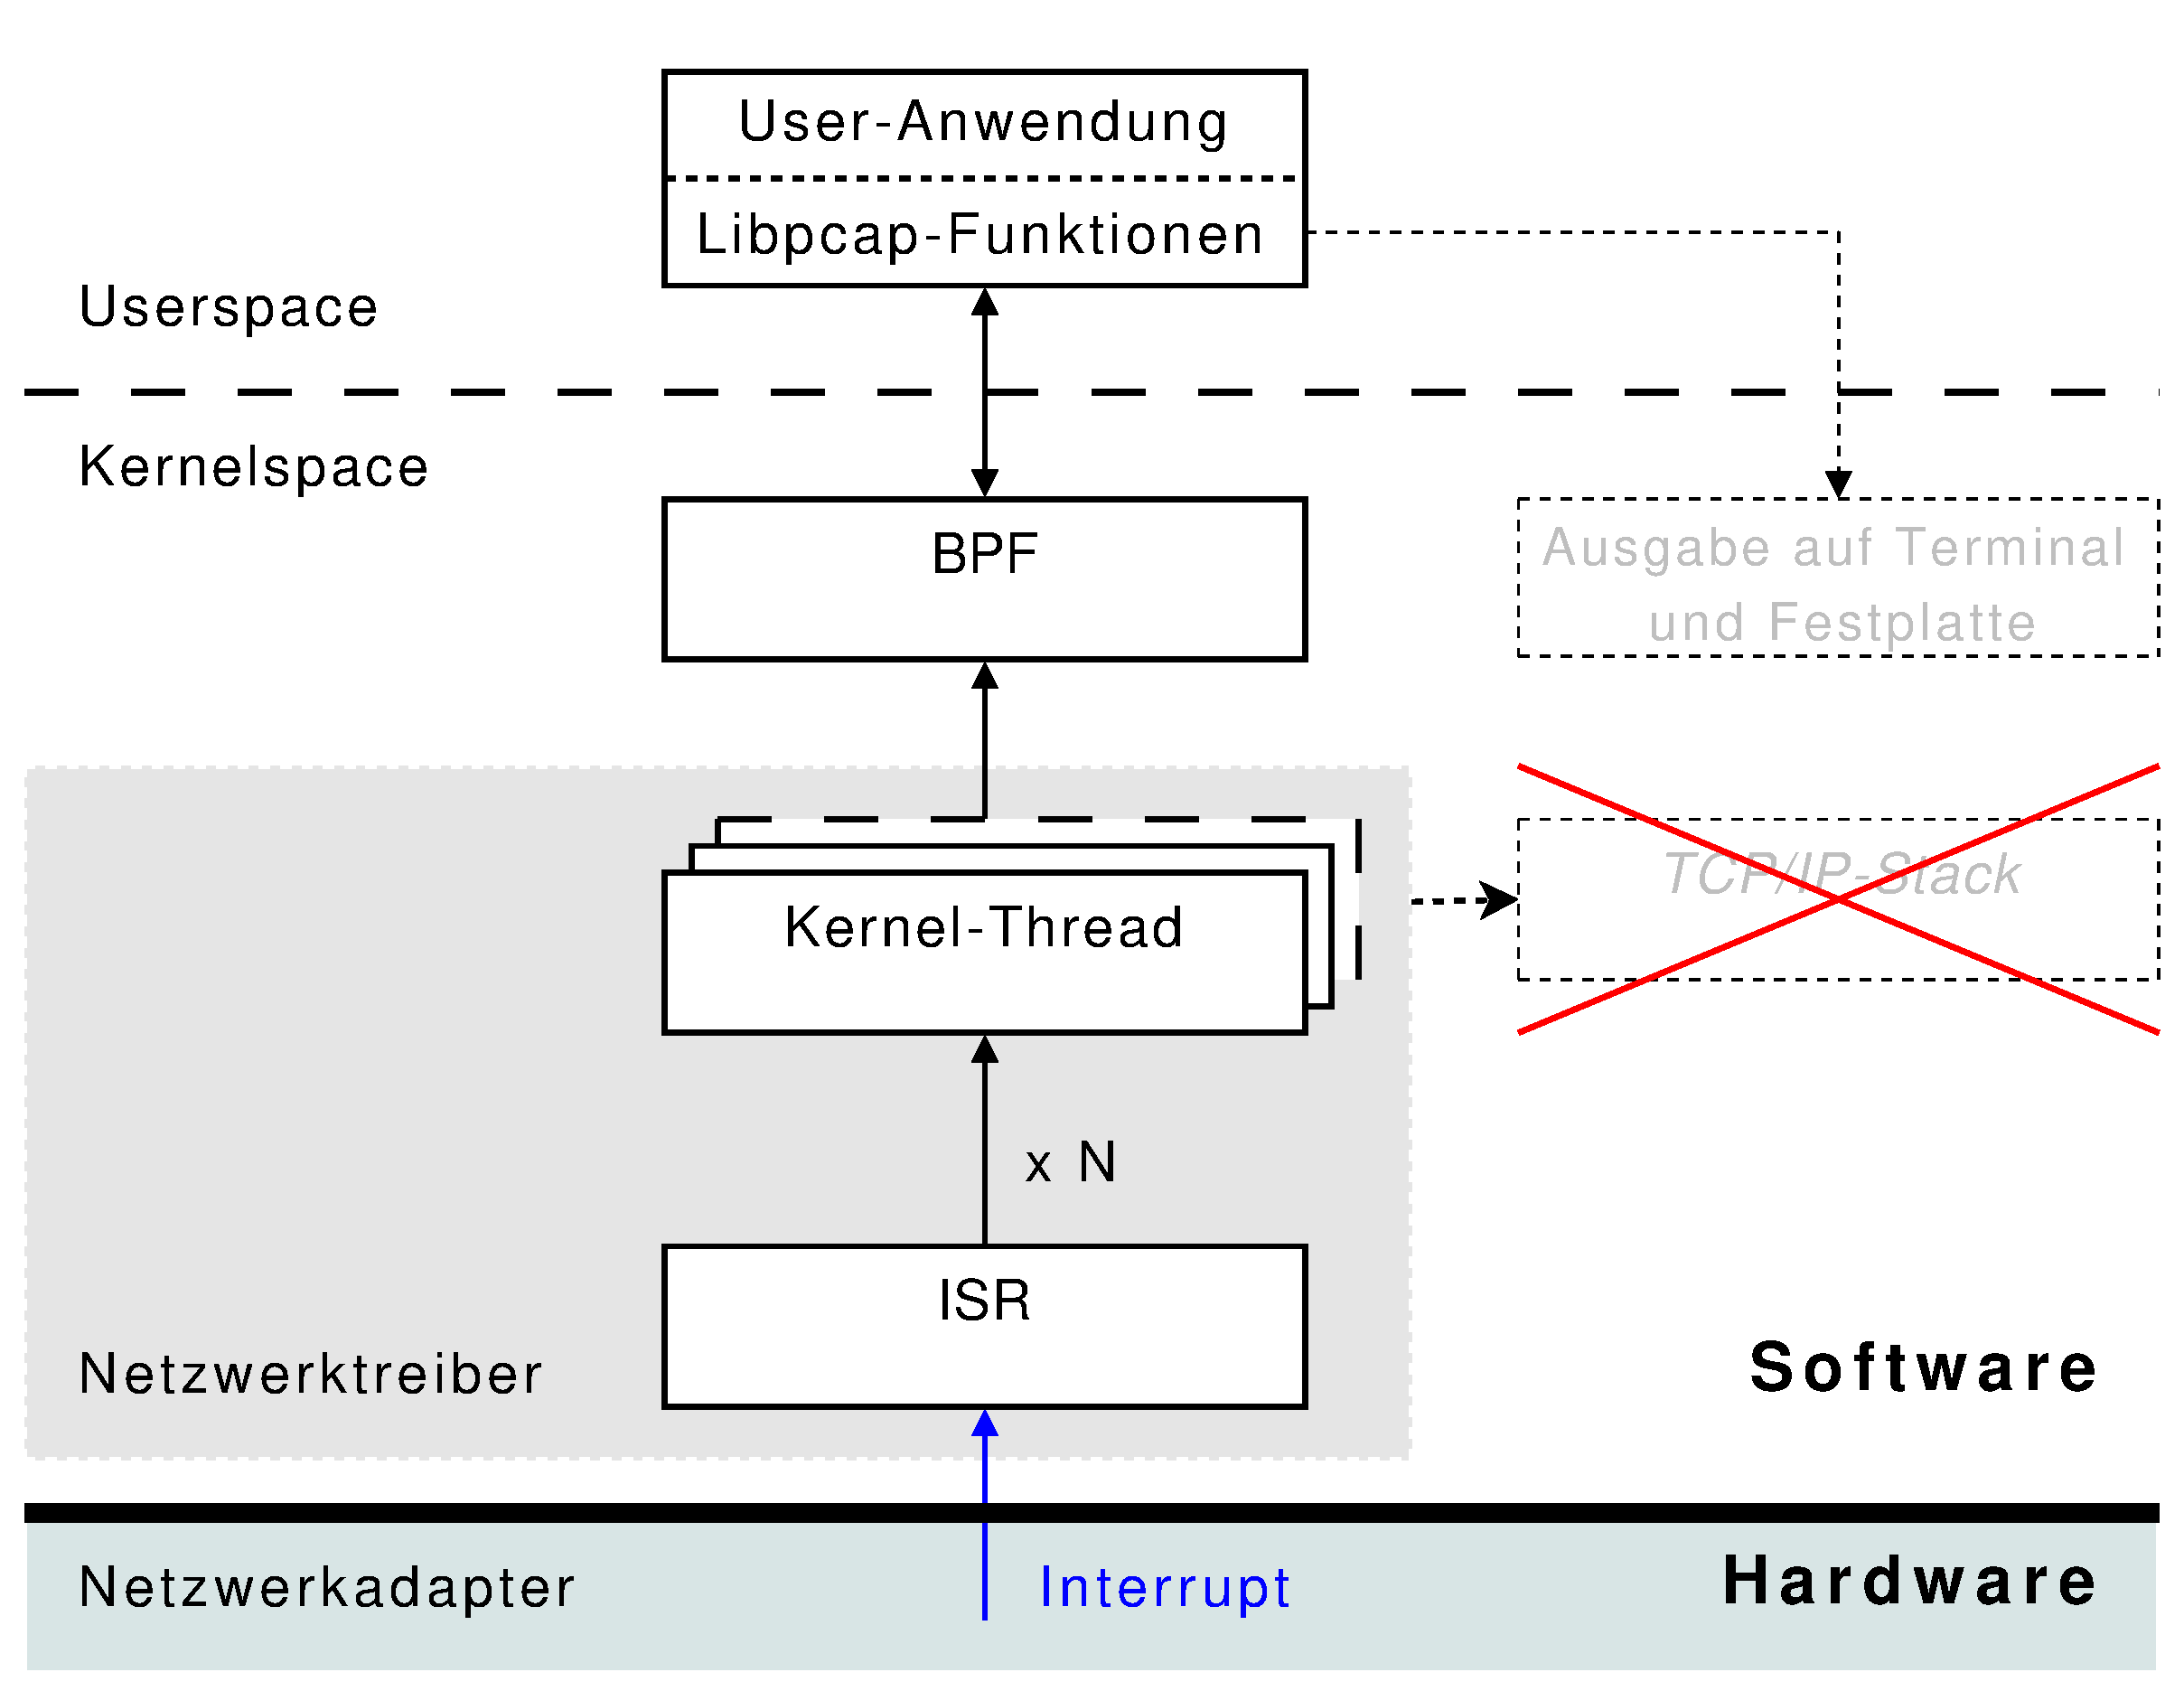
\includegraphics [height=55mm,width=60mm]{pics/PCS_funcs_ziel_DA_2}}
\only<4>{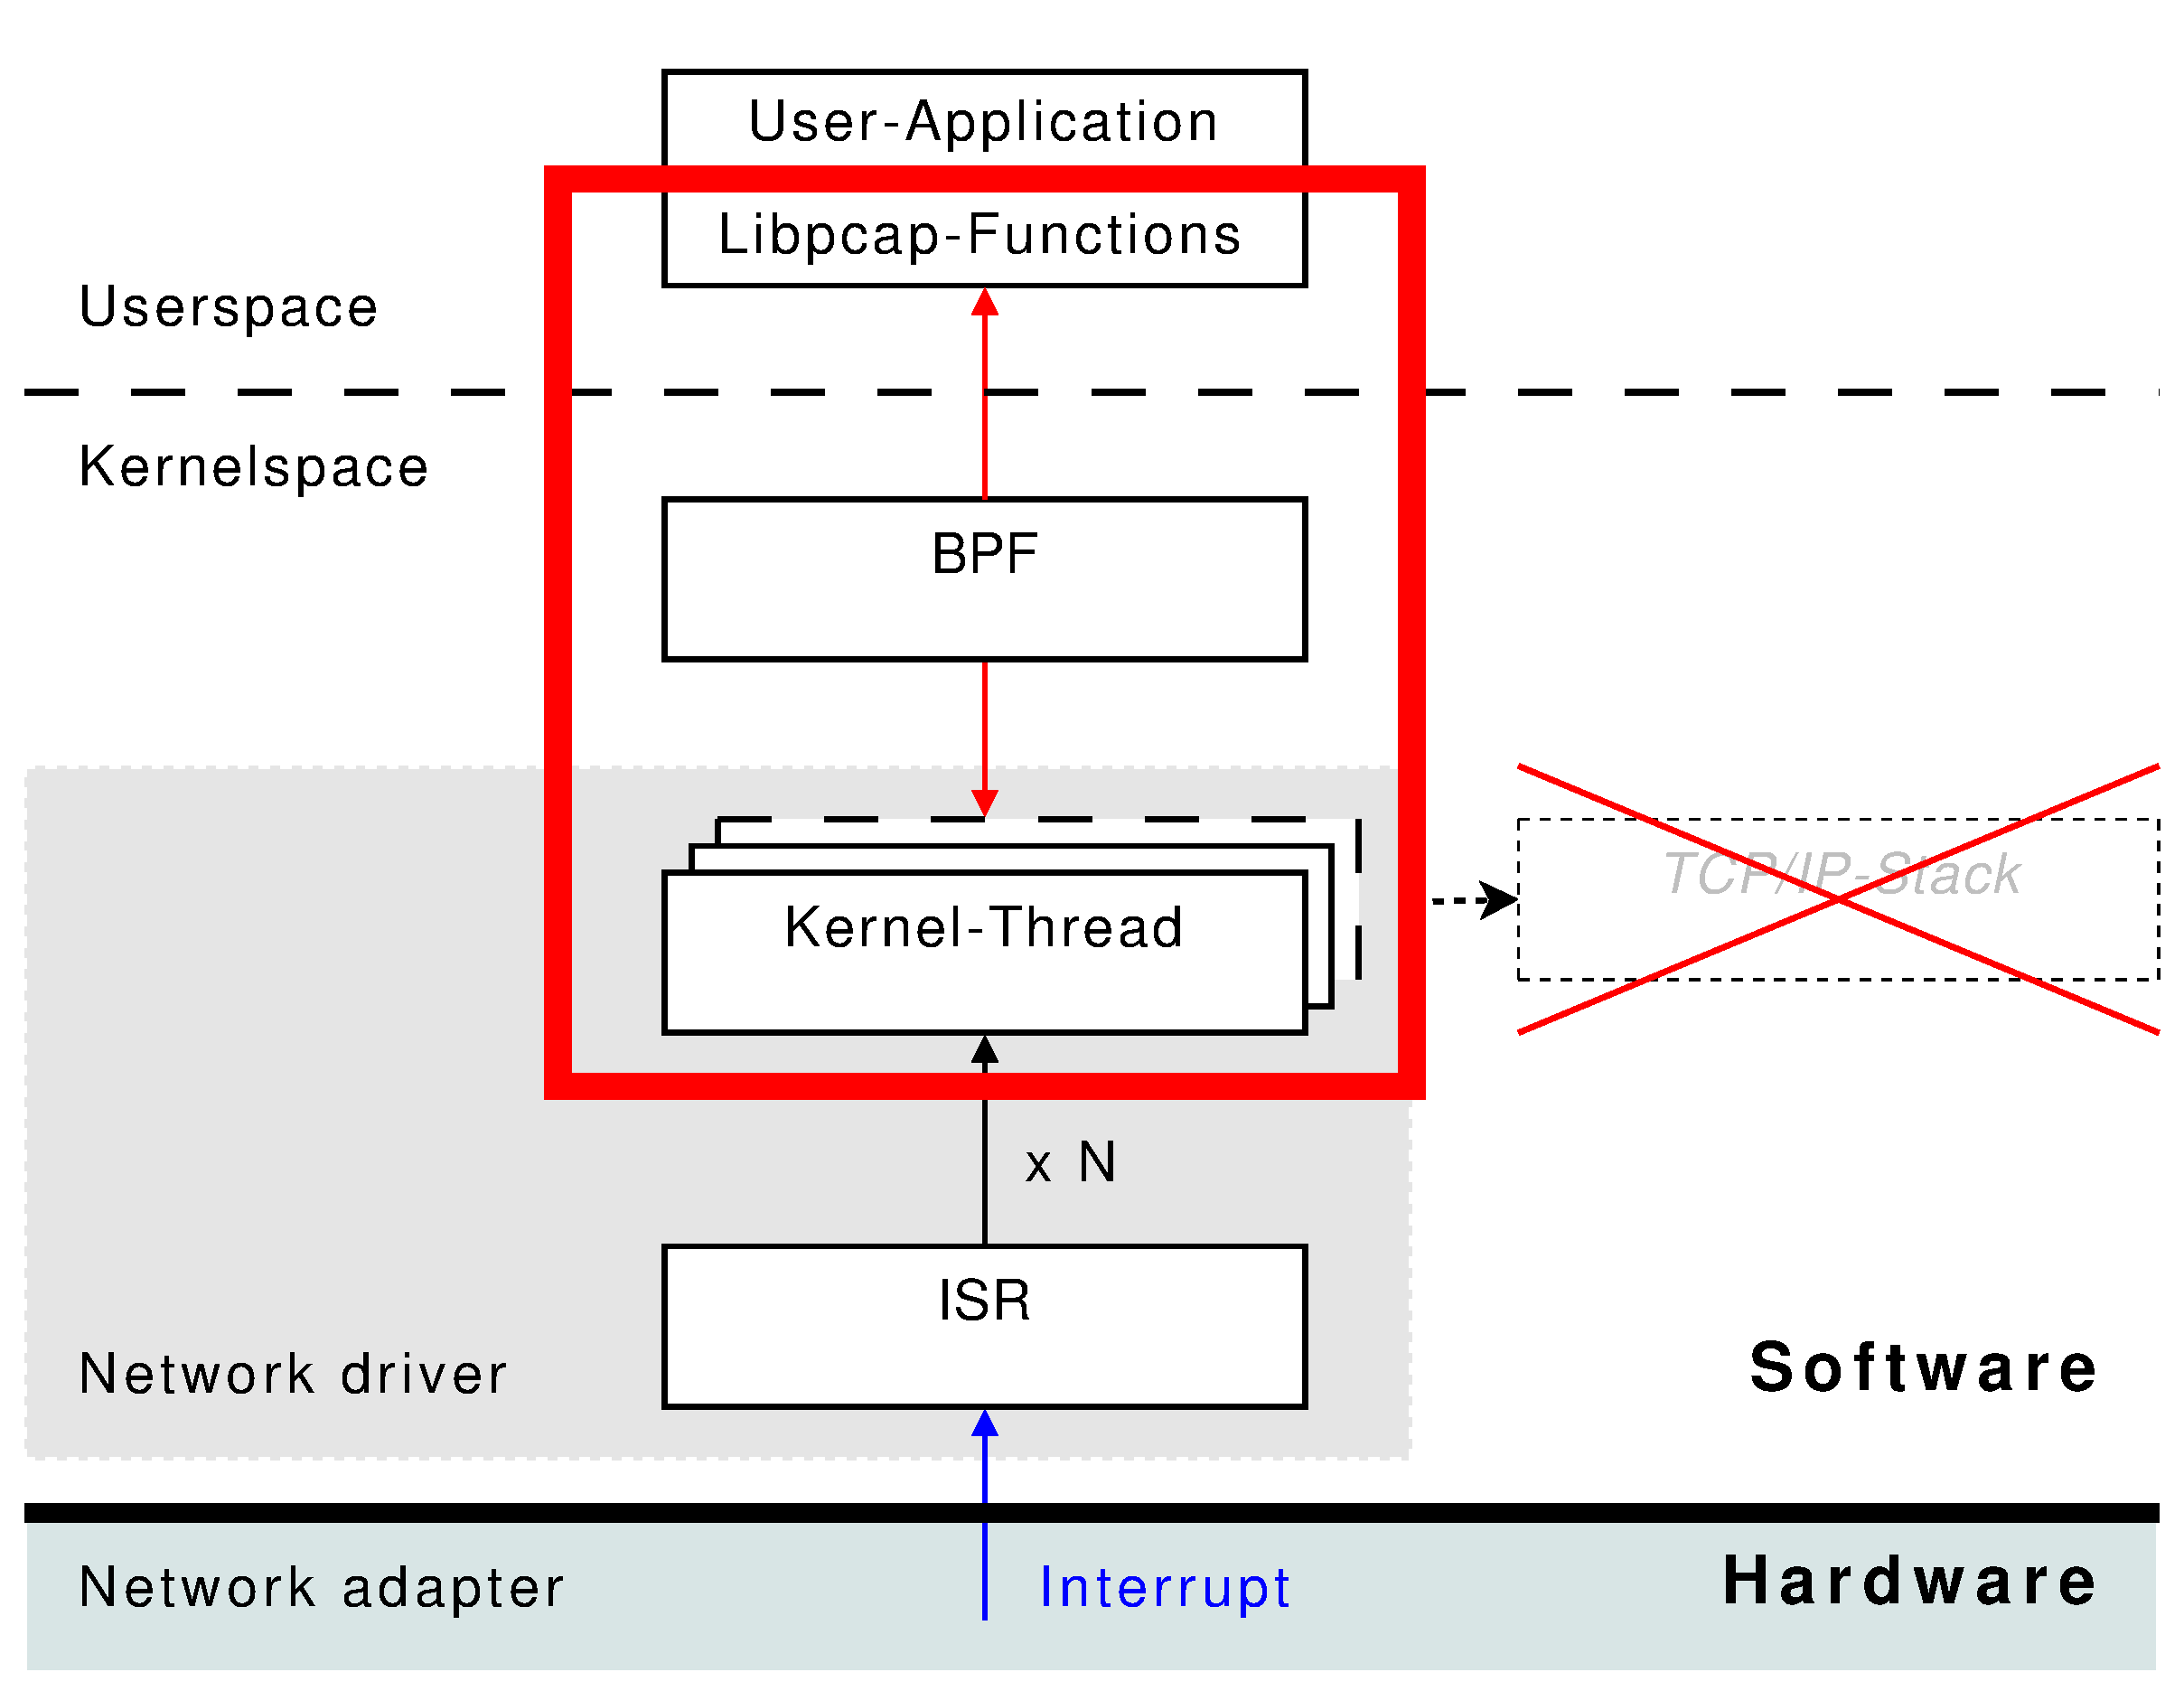
\includegraphics [height=55mm,width=60mm]{pics/PCS_funcs_ziel_DA}}
\end{columns}
\end{frame}

\subsection*{From generic to ringmap}
%%%%%%%%%%%%%%%%%%%%%%%%%%%%%%%%%%%%%%%%%%%%%%%%%%%%%%%%%%%%%%%%%%%

\begin{frame}
	\begin{center}
		\huge{From \emph{generic} to \emph{ringmap}}
	\end{center}
\end{frame}

%%%%%%%%%%%%%%%%%%%%%%%%%%%%%%%%%%%%%%%%%%%%%%%%%%%%%%%%%%%%%%%%%%%
\begin{frame}
\frametitle{From generic to ringmap}
\begin{columns}
\column[t]{0.5\textwidth}
\vspace{-1em}
\begin{itemize}
	\item<1->\textbf{generic}
	\item<2->Eliminate packet copies  and syscalls
	\item<3->BPF-Buffer is then not necessary
		\begin{itemize}
			\item<3->Packet filtering is possible in both kernel and 
				user-space
		\end{itemize}
	\item<4->Mapping the Packet-Buffer to user-space
	\item<5->[$\Rightarrow$]\textbf{ringmap}
\end{itemize}
\column[t]{0.5\textwidth}
\vspace{-2em}
\only<1>{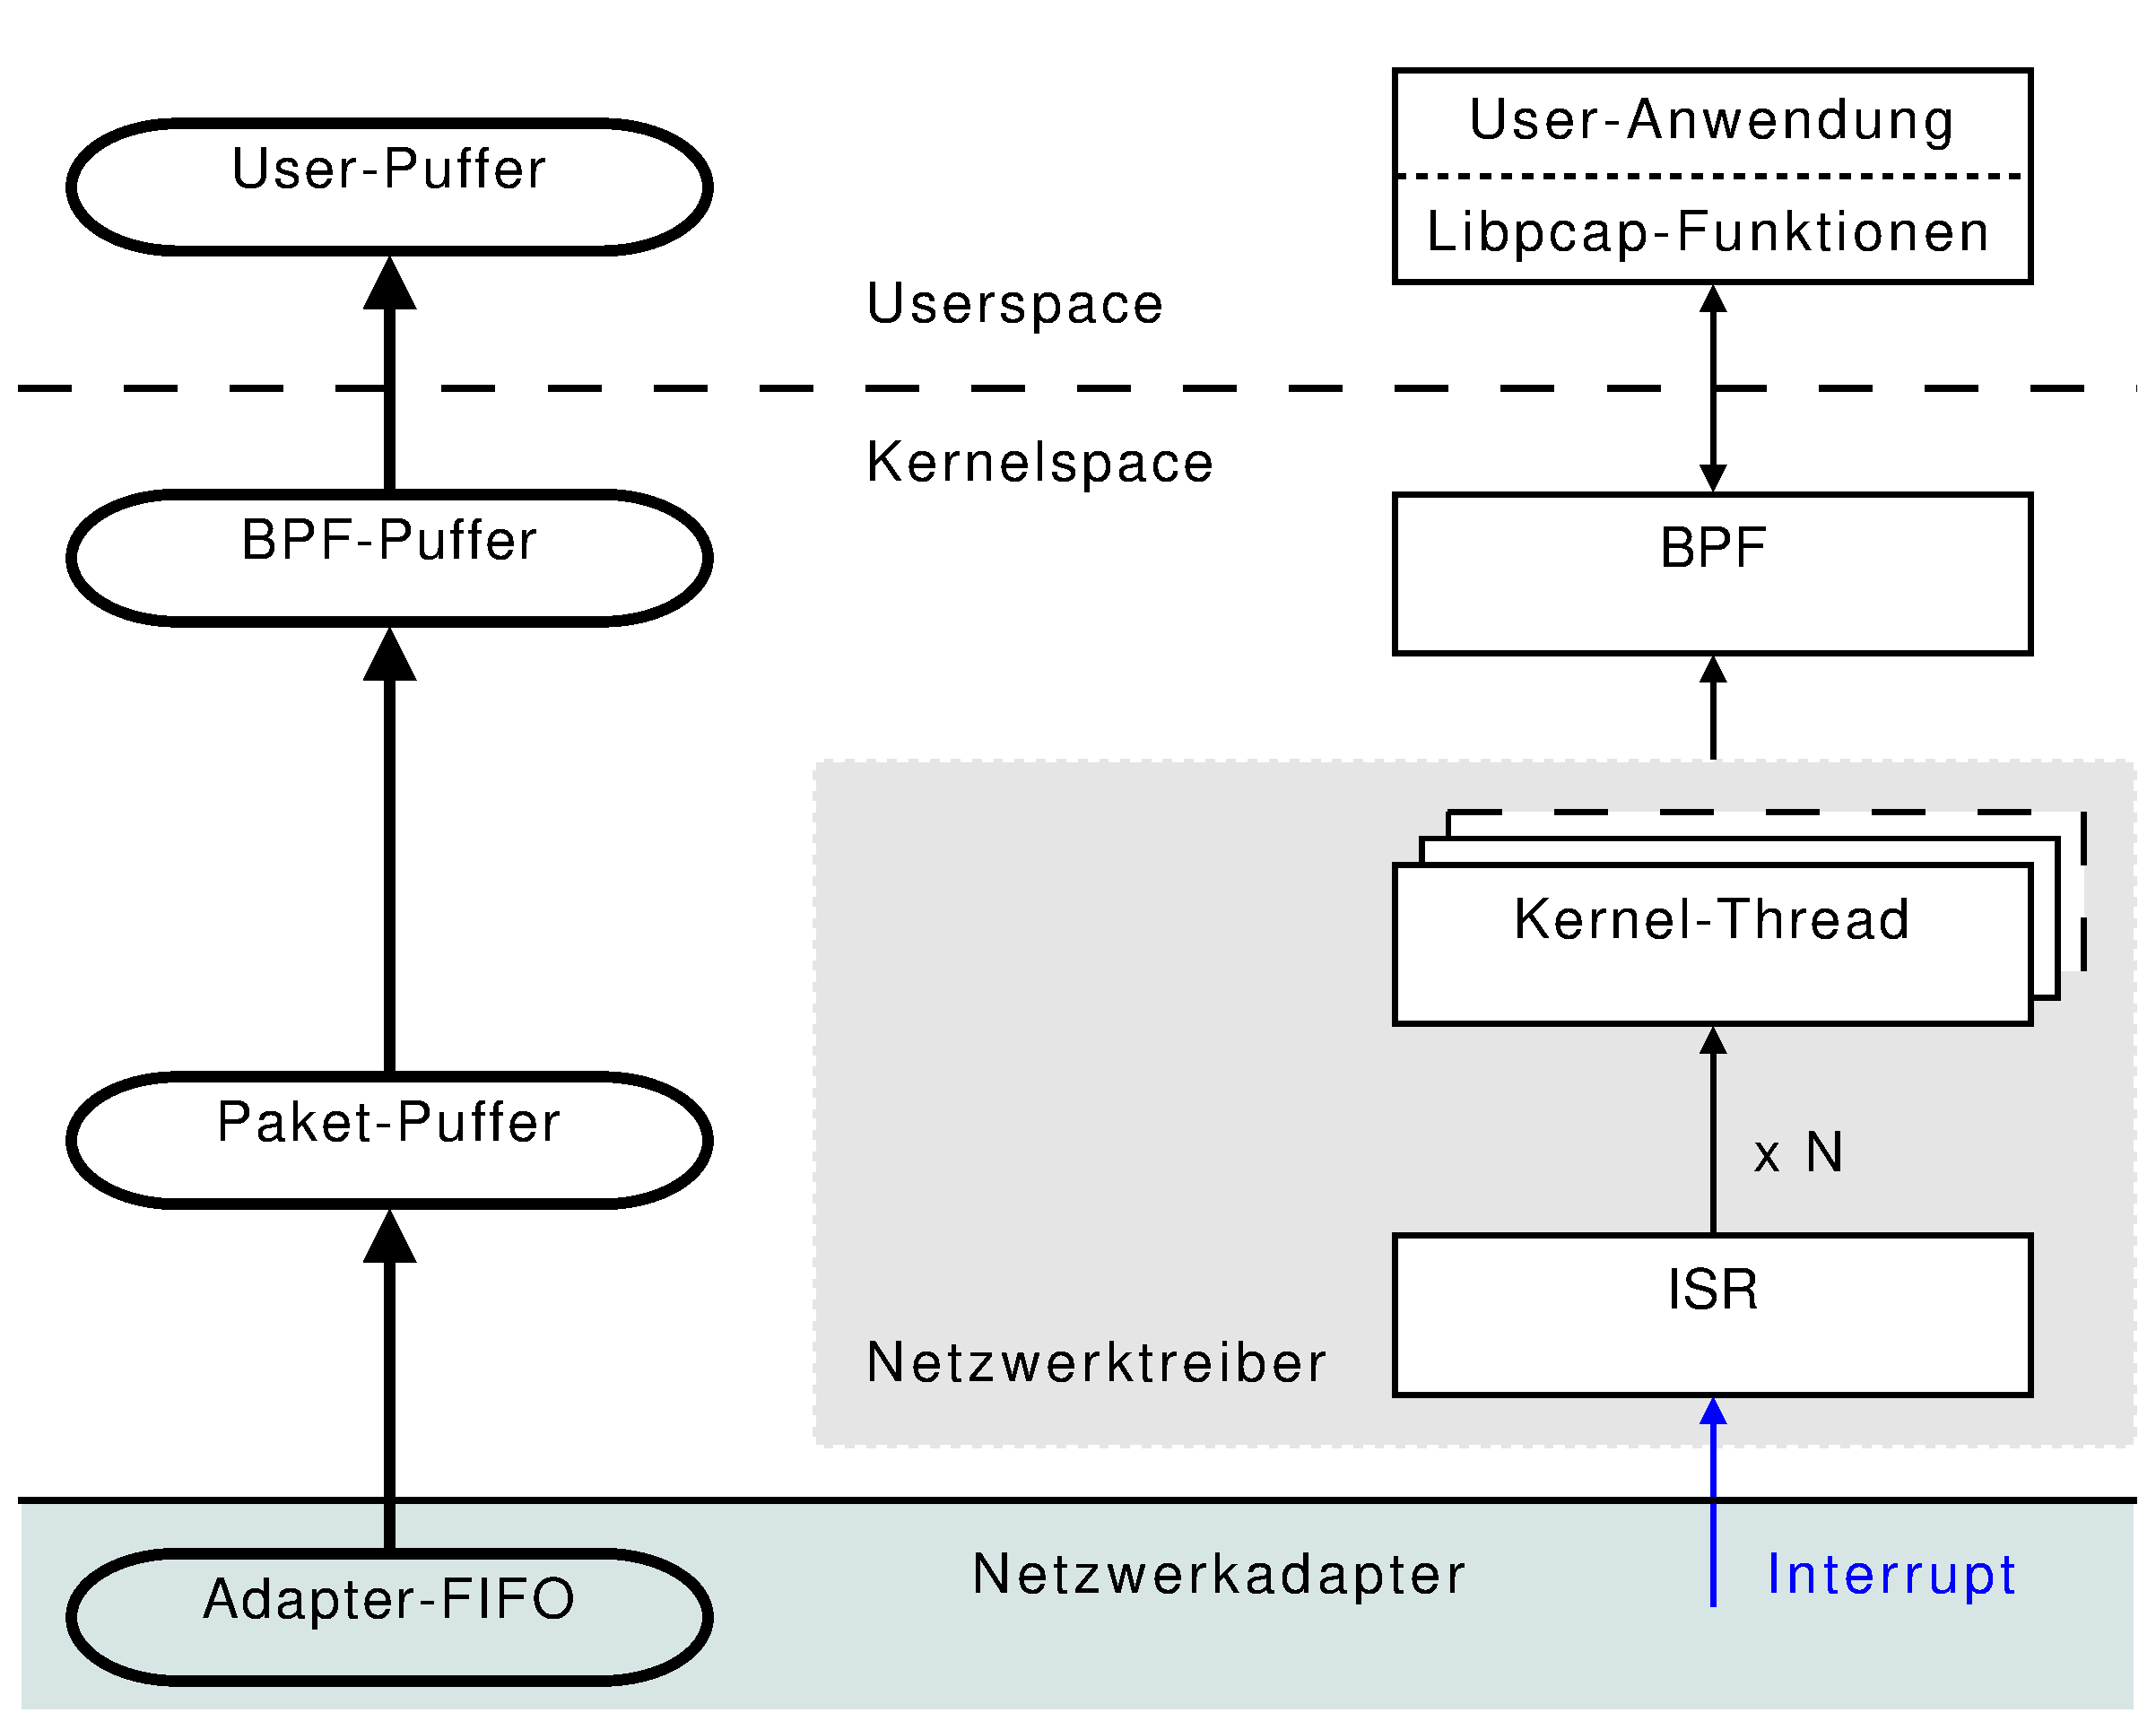
\includegraphics [height=59mm,width=60mm]{pics/3copy}}
\only<2>{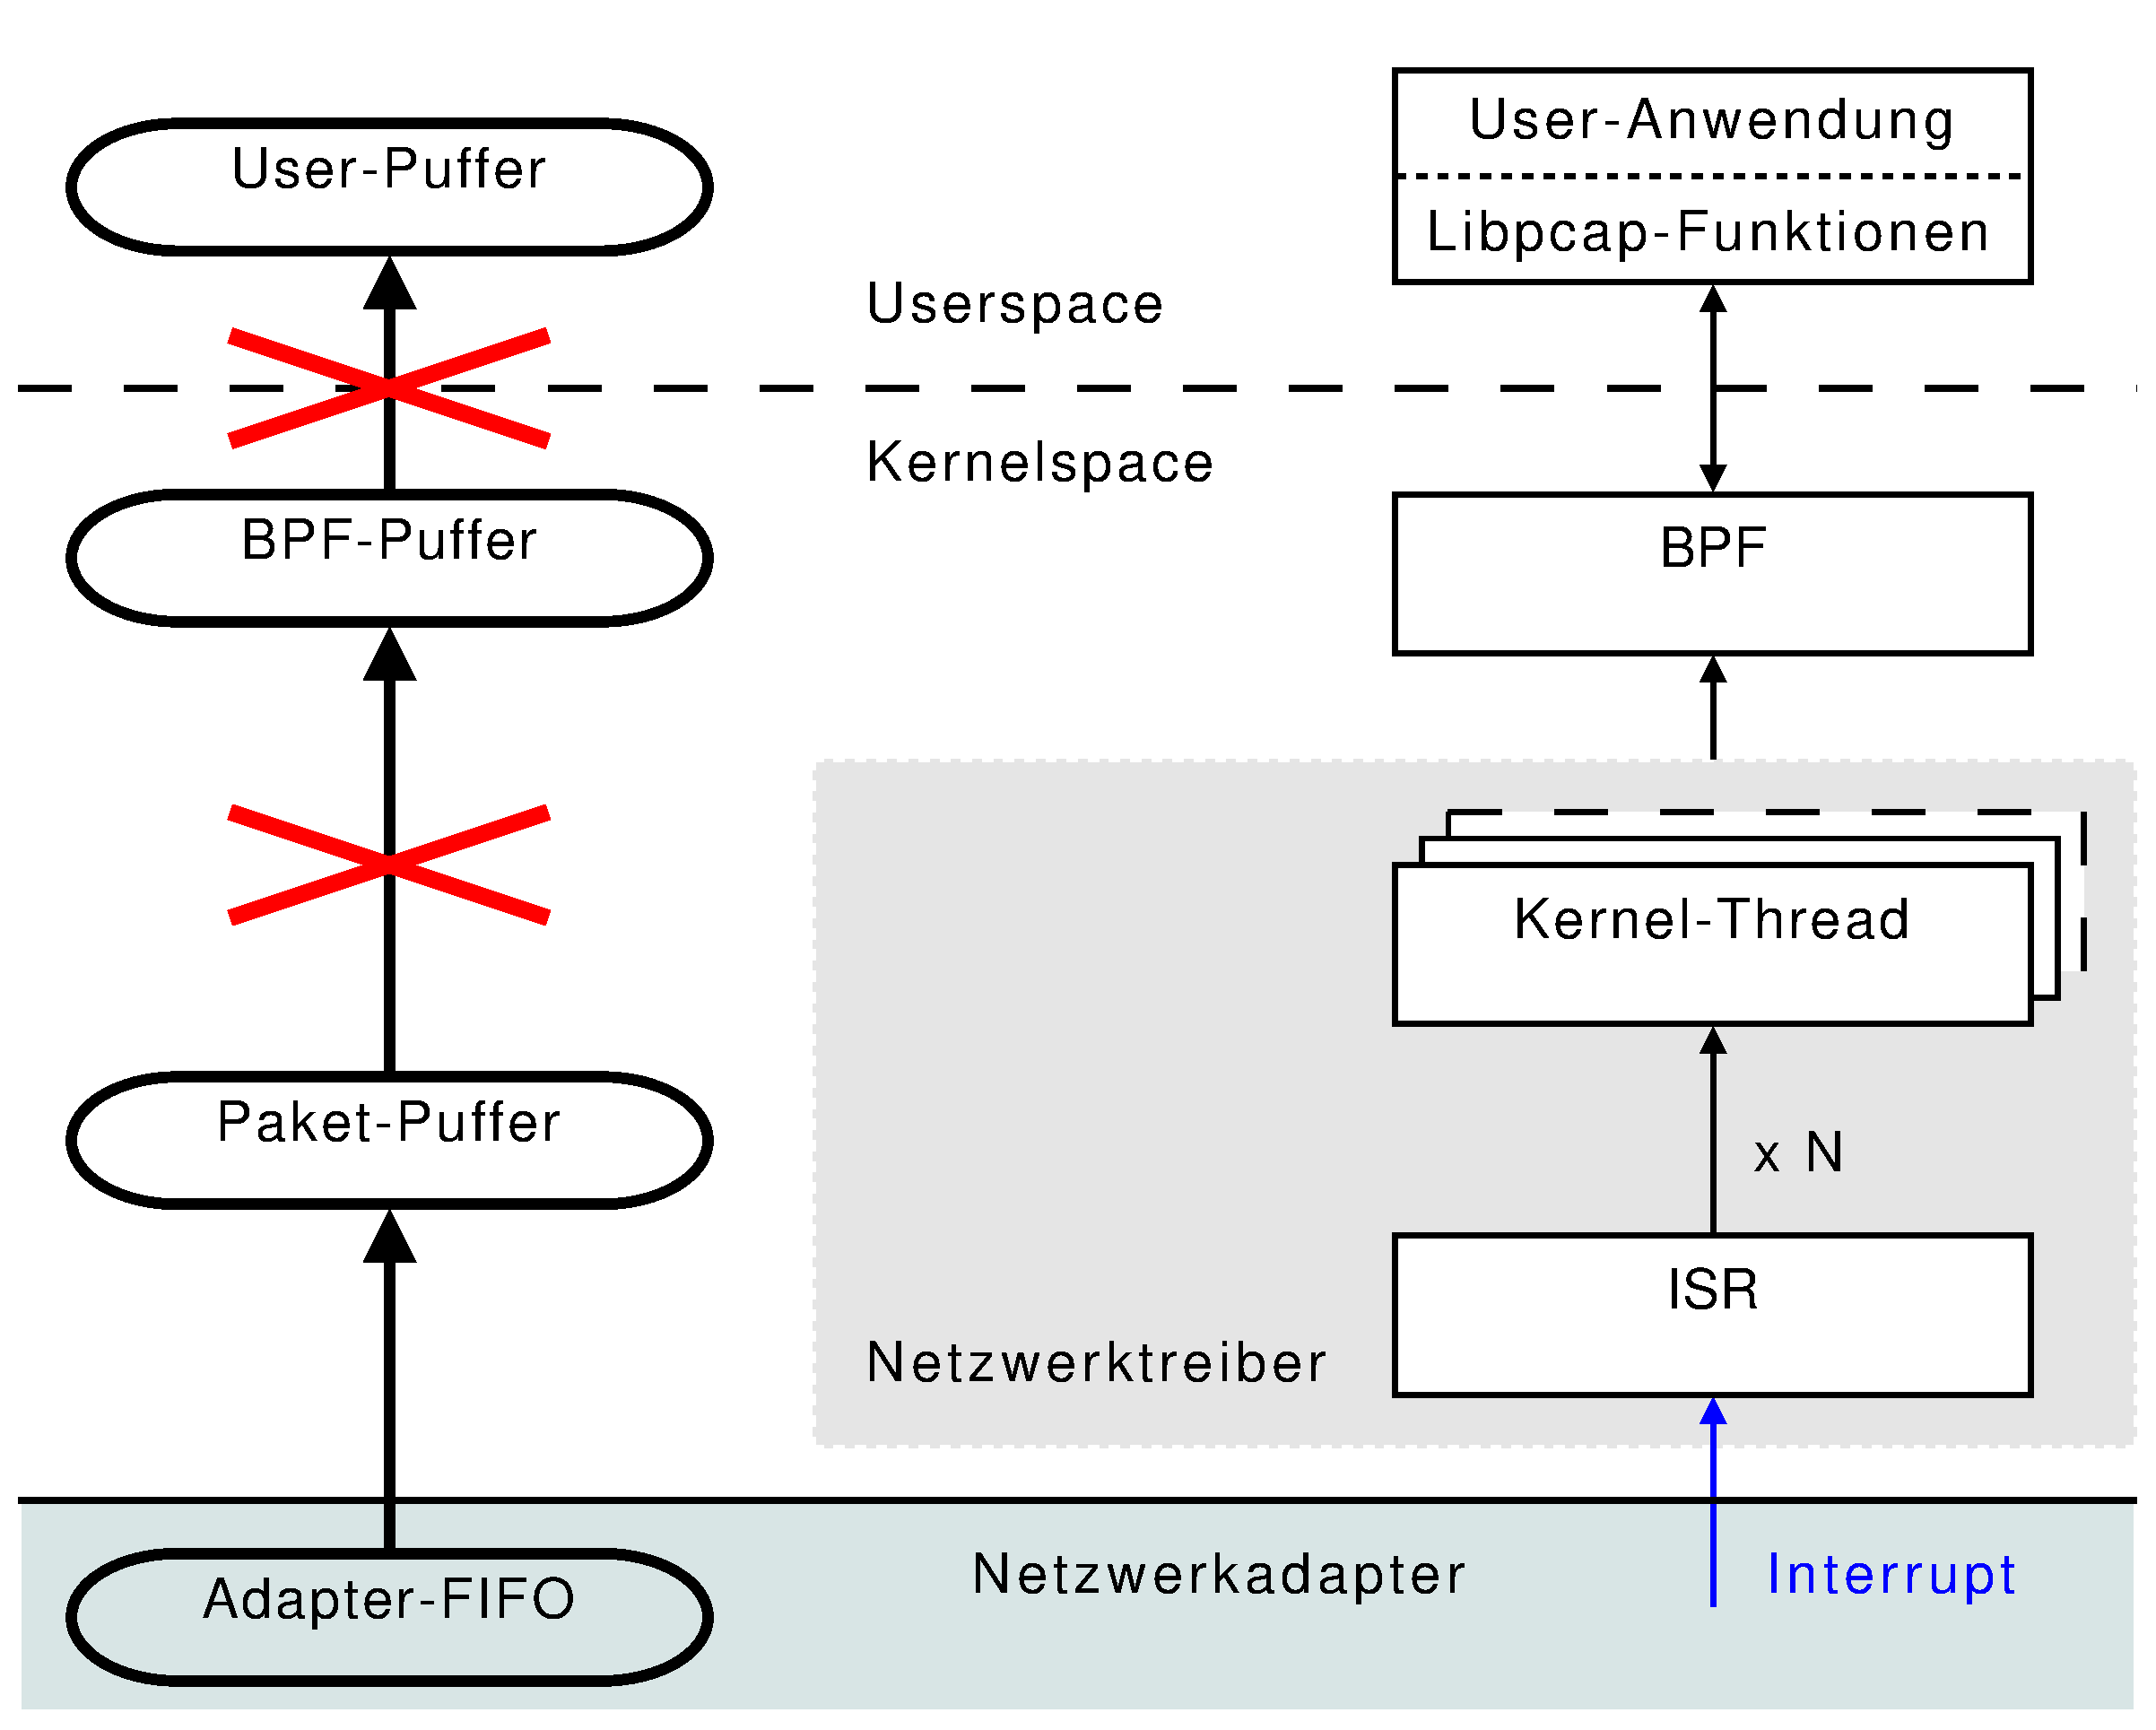
\includegraphics [height=59mm,width=60mm]{pics/3copy_solution_1}}
\only<3>{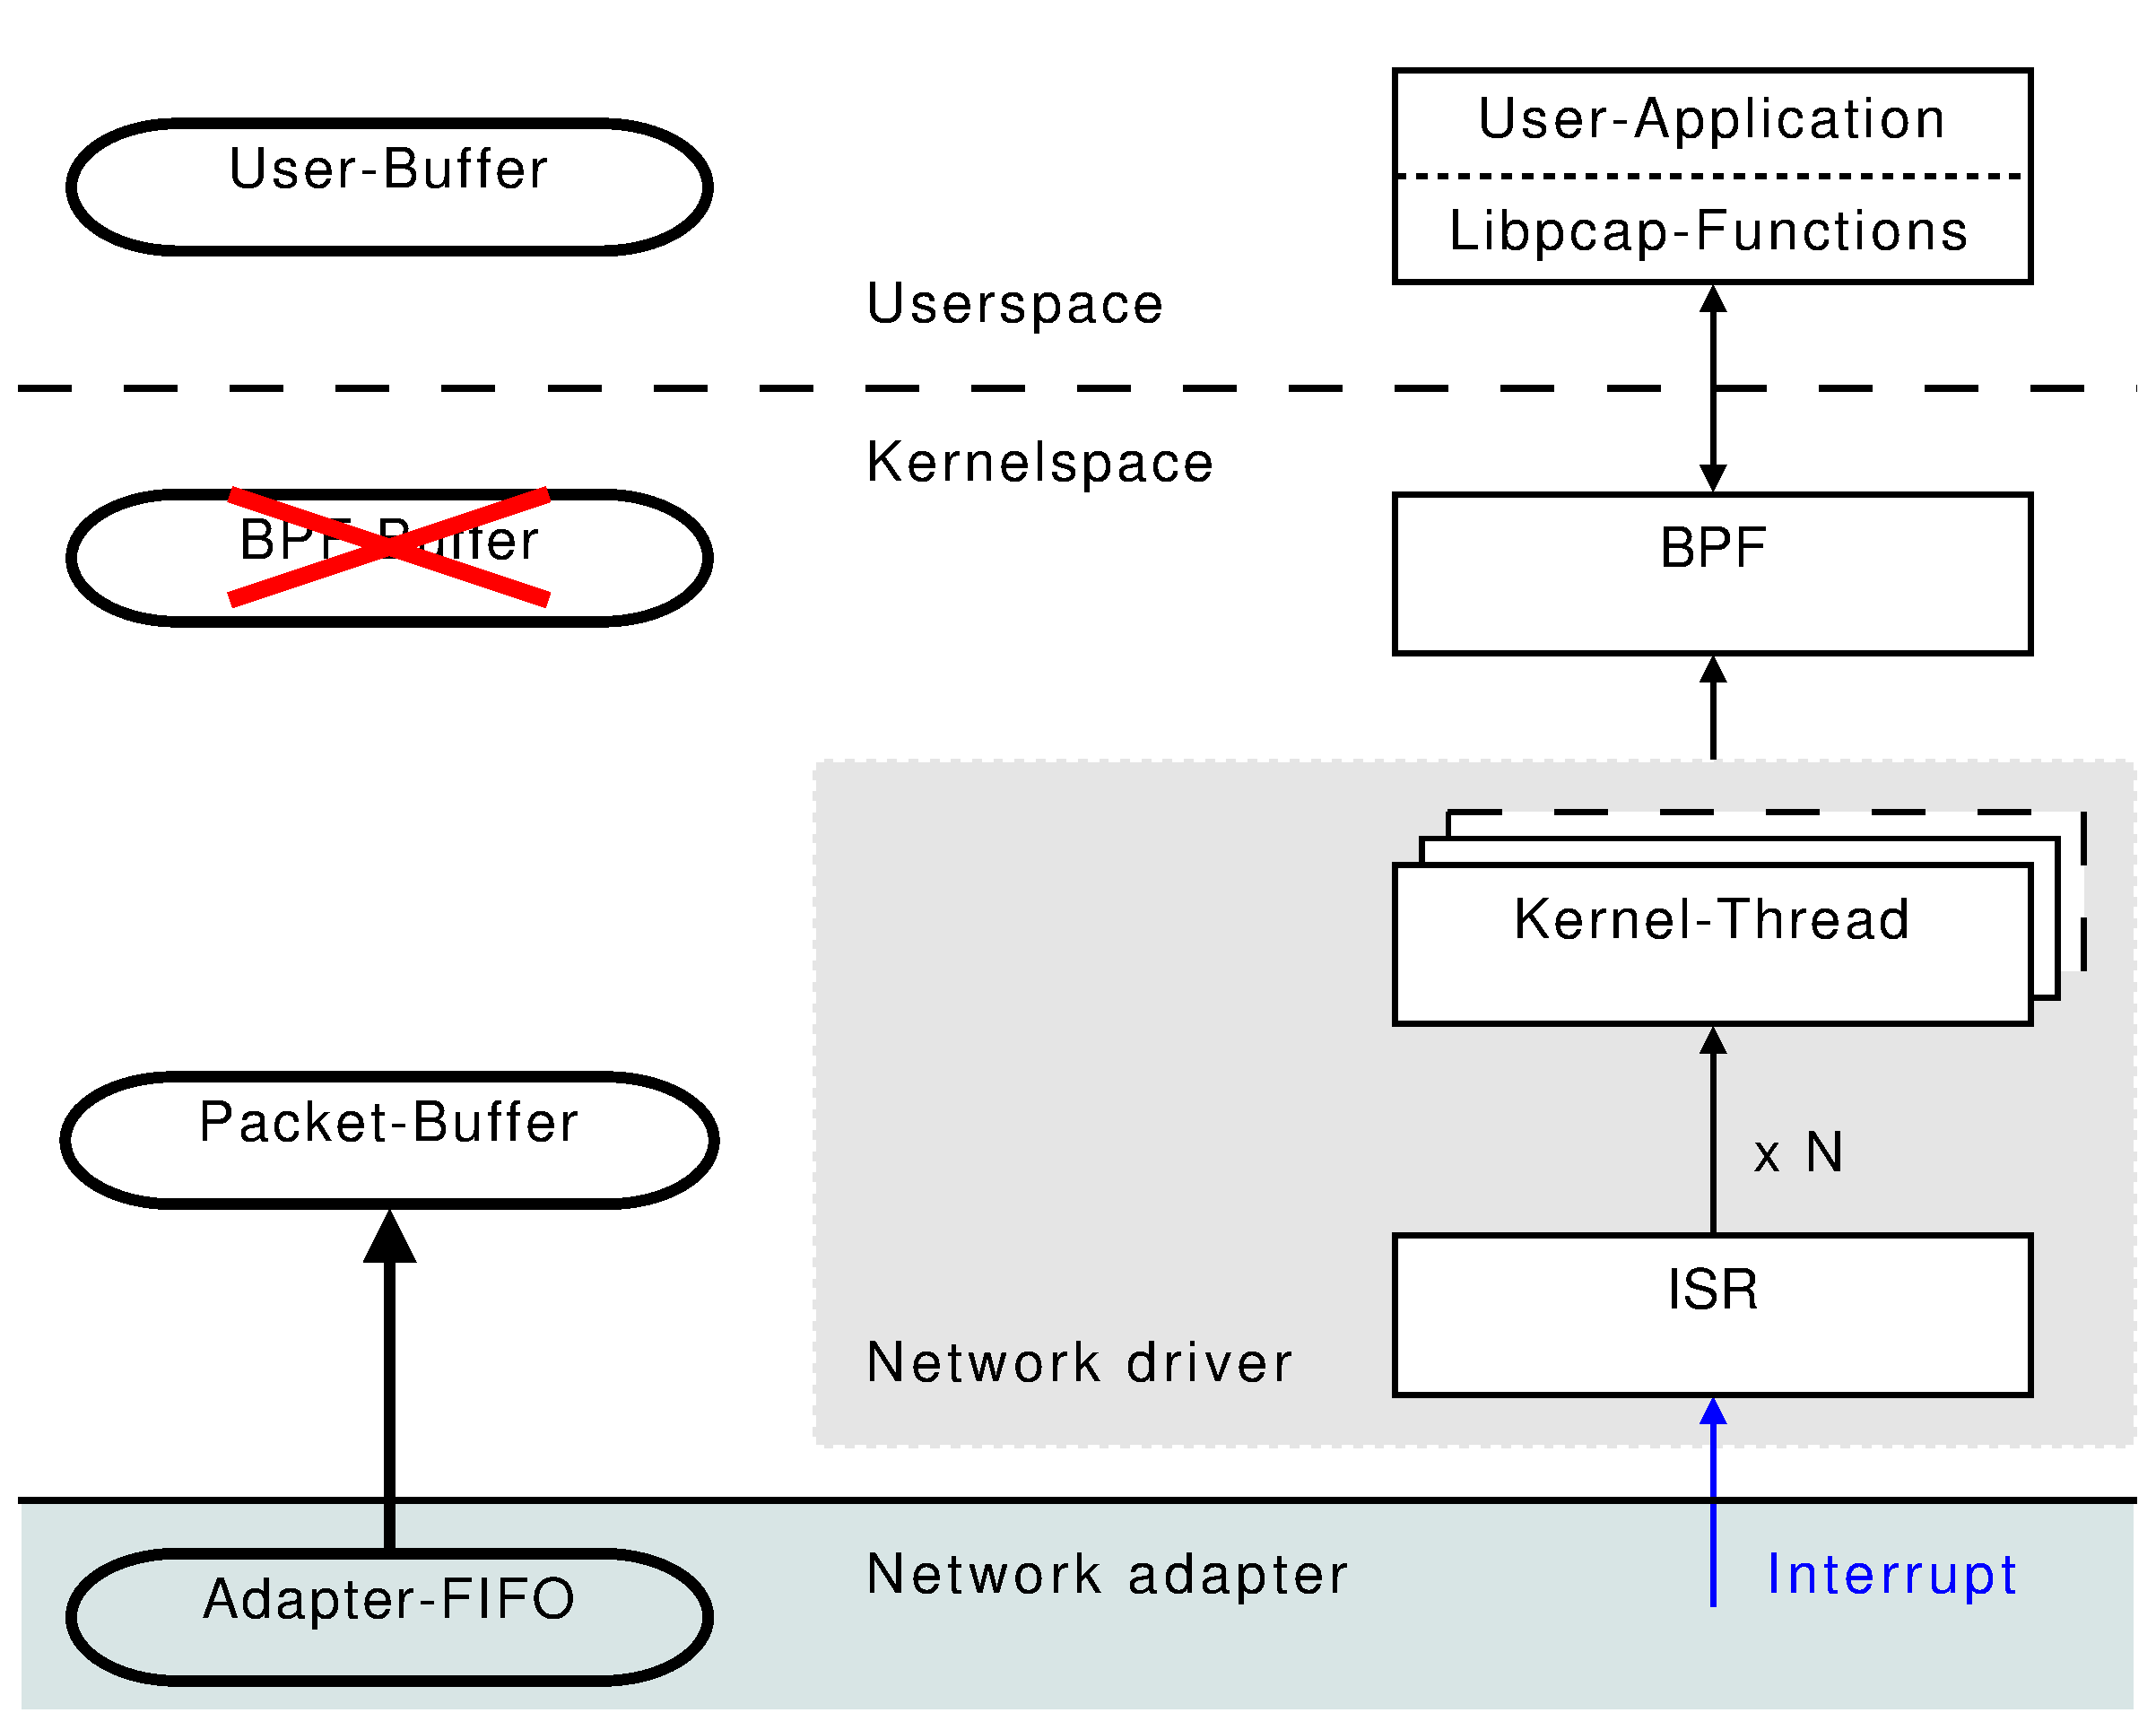
\includegraphics [height=59mm,width=60mm]{pics/3copy_solution_2}}
\only<4>{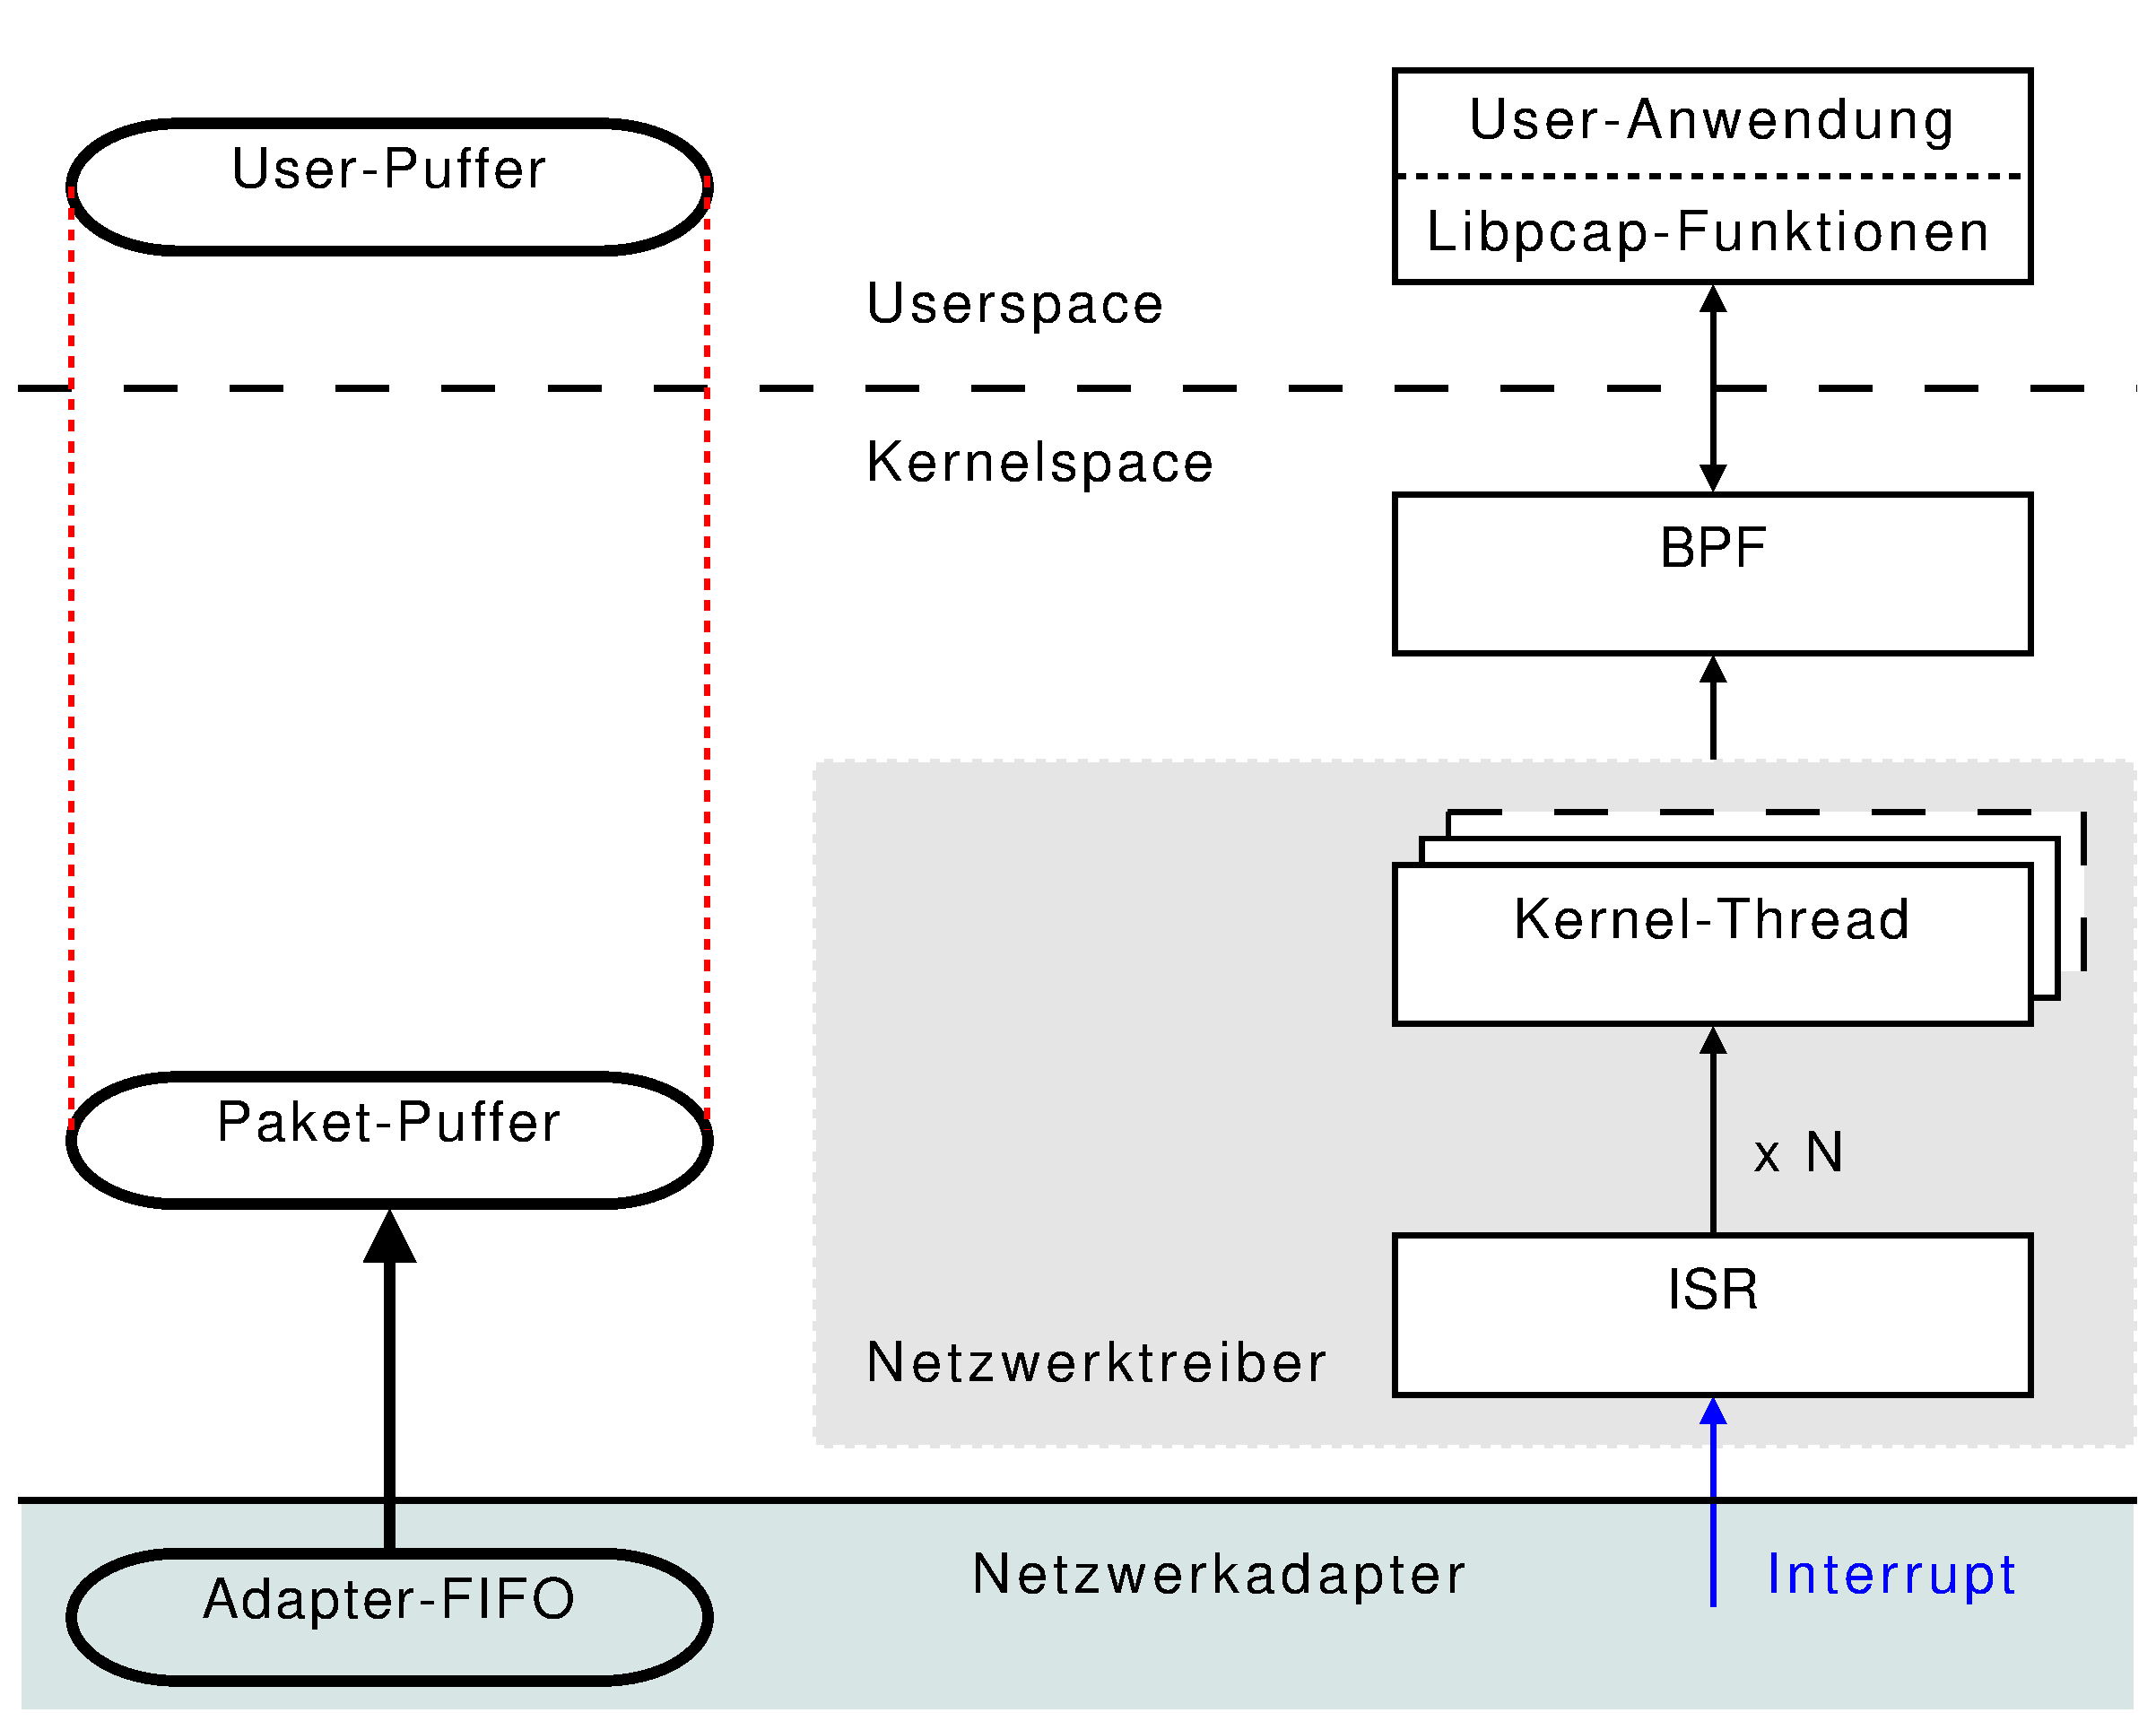
\includegraphics [height=59mm,width=60mm]{pics/3copy_solution_3}}
%\only<5>{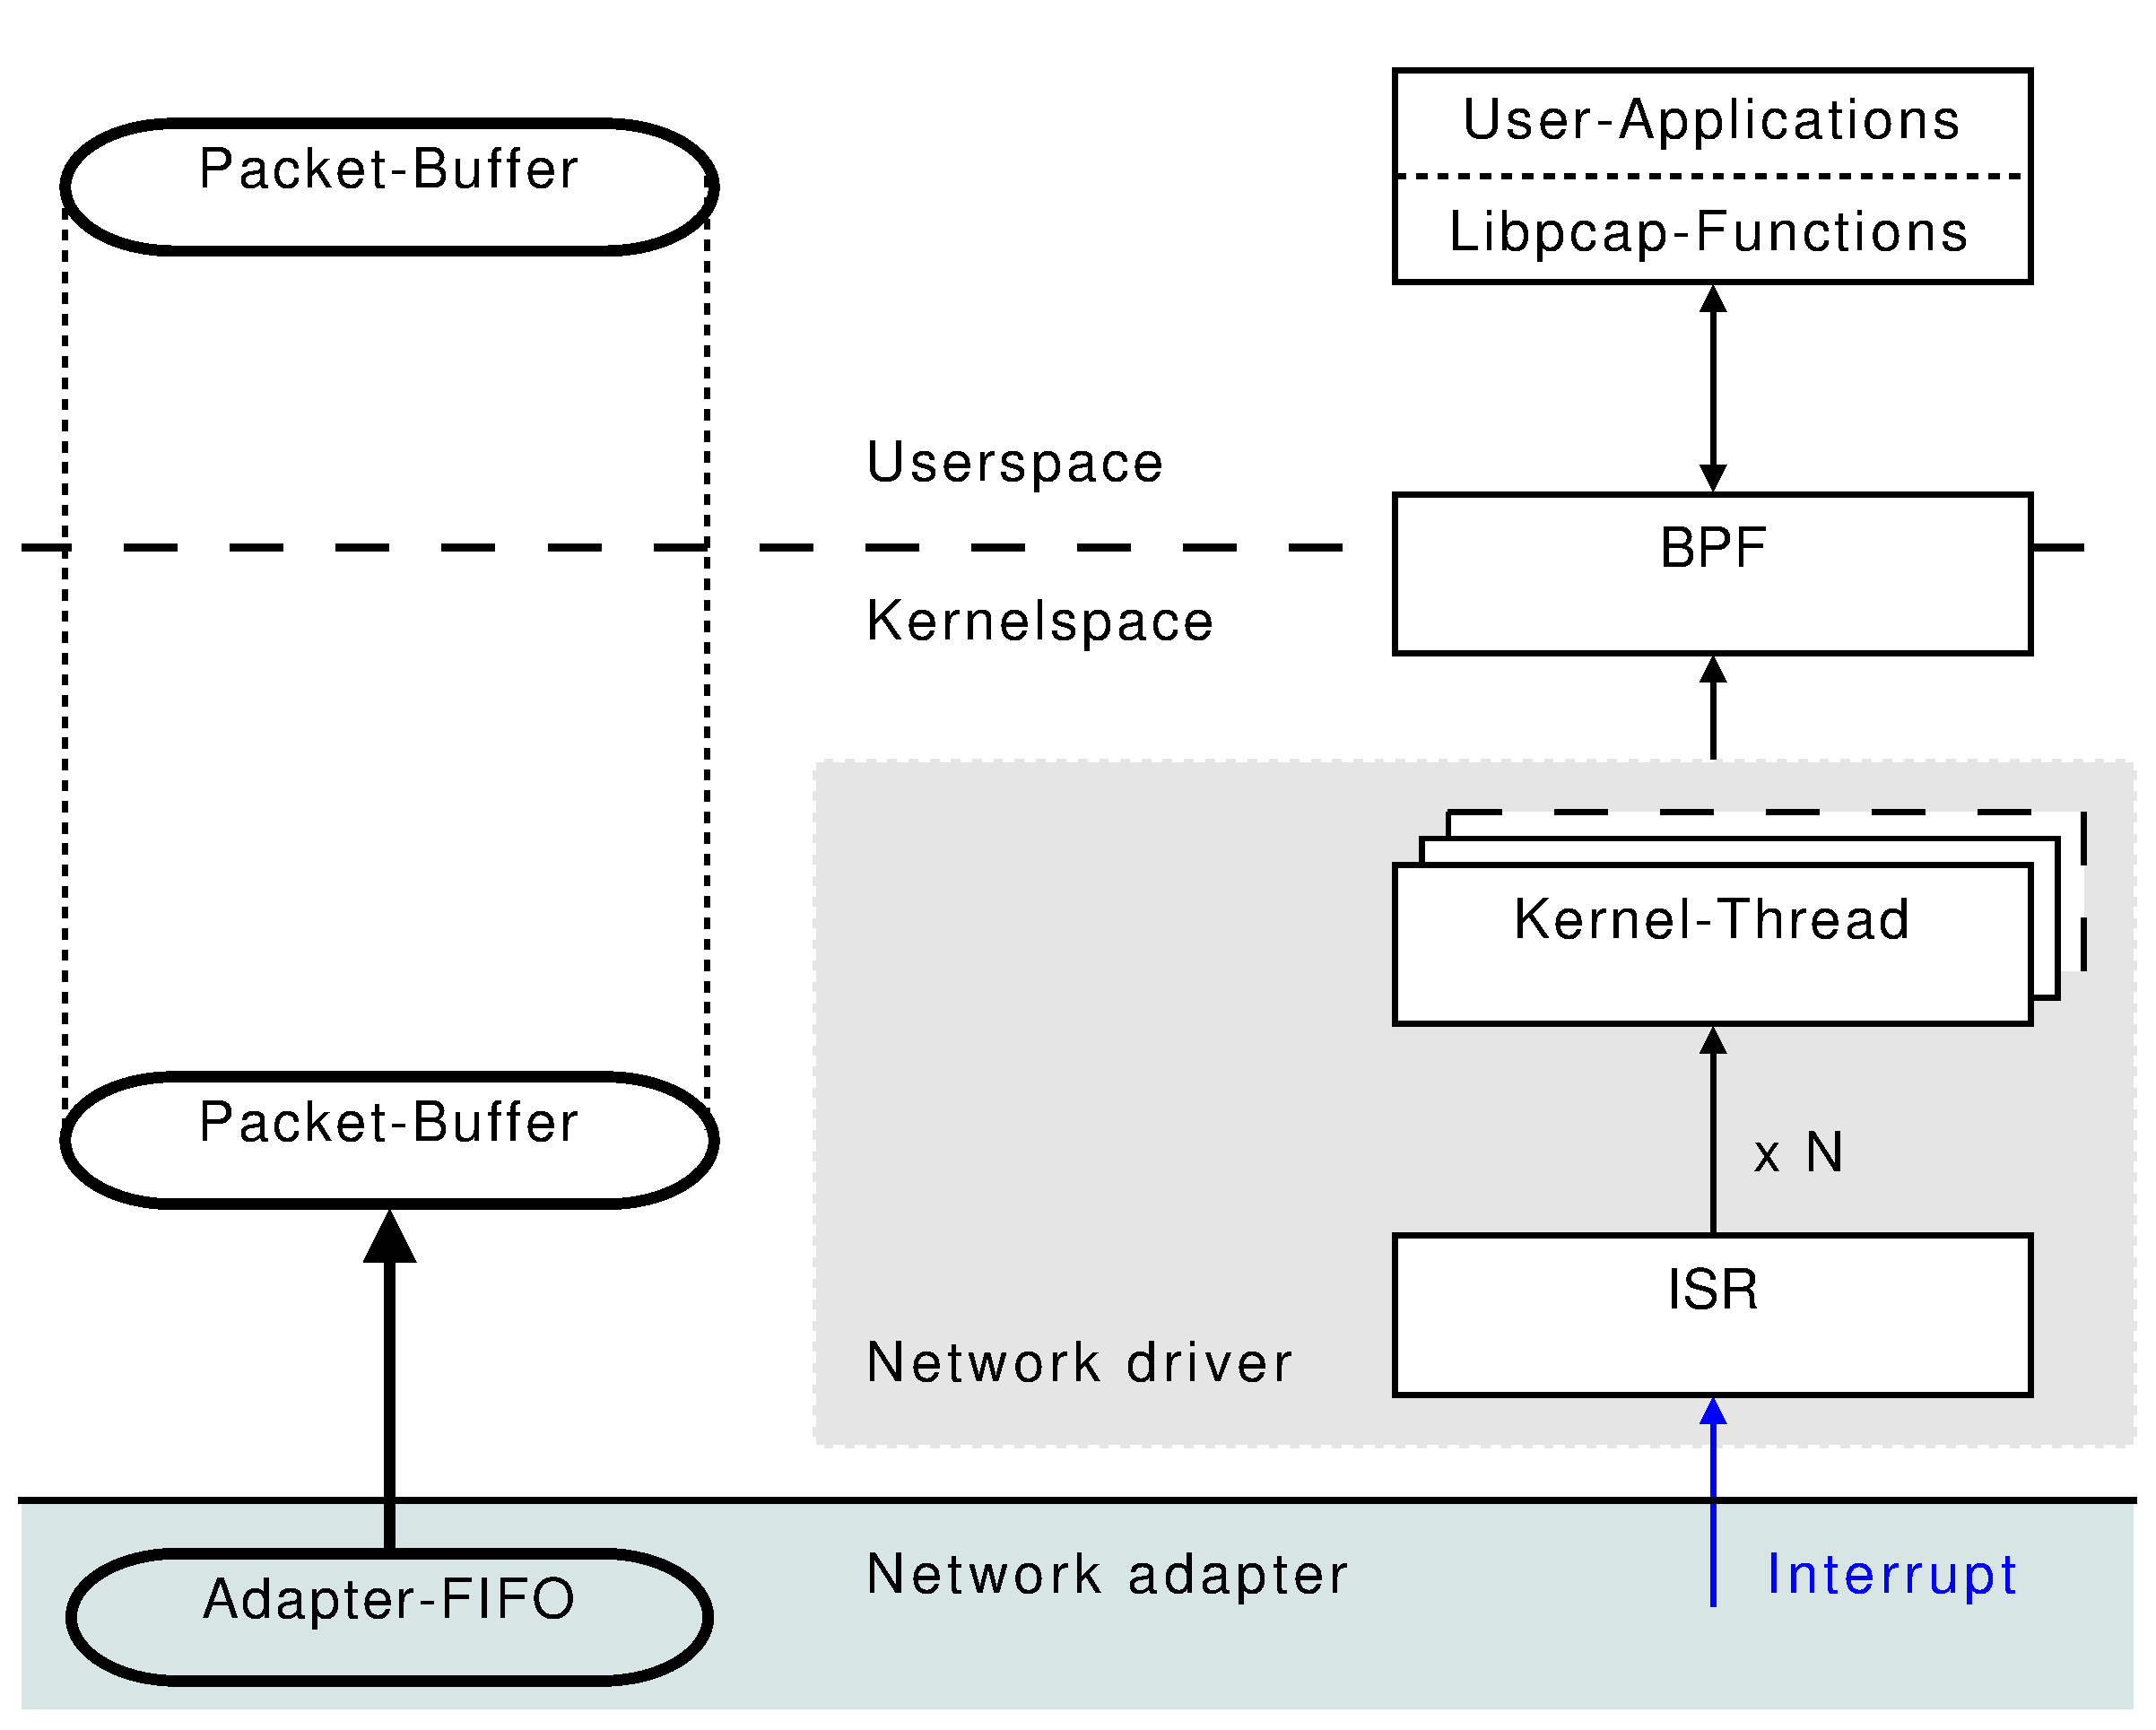
\includegraphics [height=59mm,width=60mm]{pics/3copy_solution_4}}
\only<5>{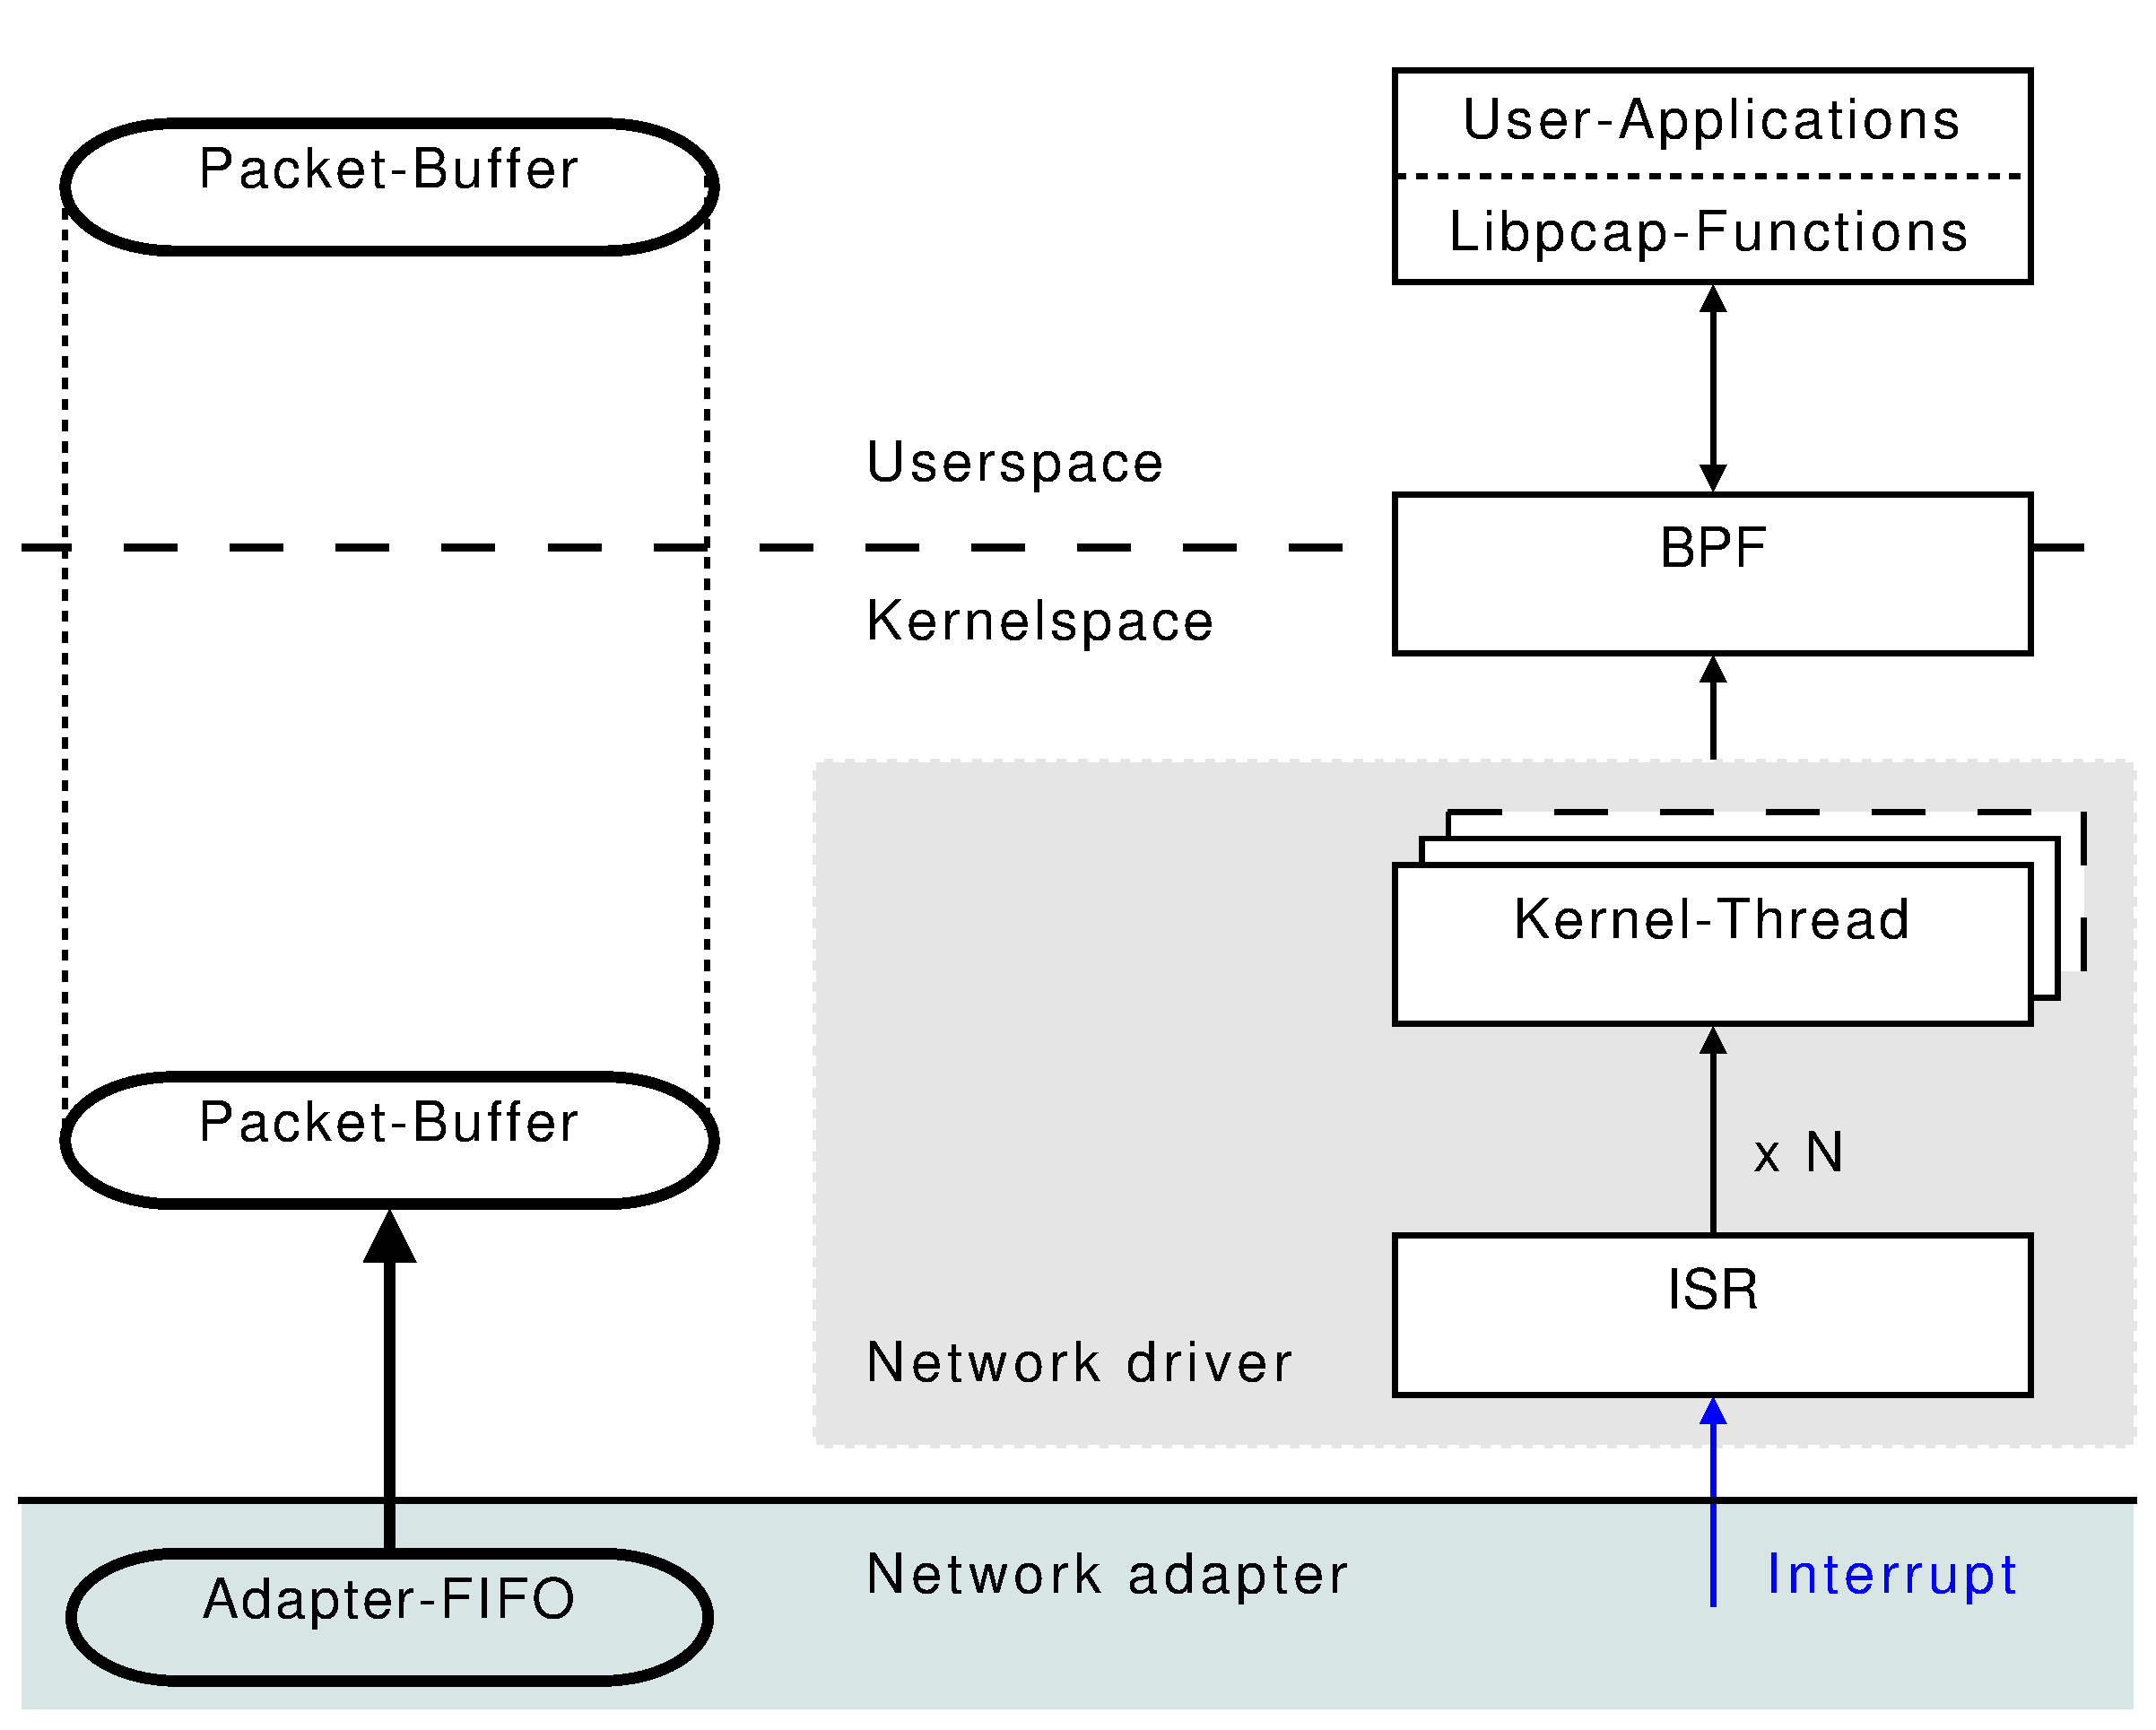
\includegraphics [height=59mm,width=60mm]{pics/3copy_solution_4}}
\end{columns}
\end{frame}

\subsection*{Overview}
%%%%%%%%%%%%%%%%%%%%%%%%%%%%%%%%%%%%%%%%%%%%%%%%%%%%%%%%%%%%%%%%%%%
\begin{frame}
\frametitle{Overview}
\begin{center}
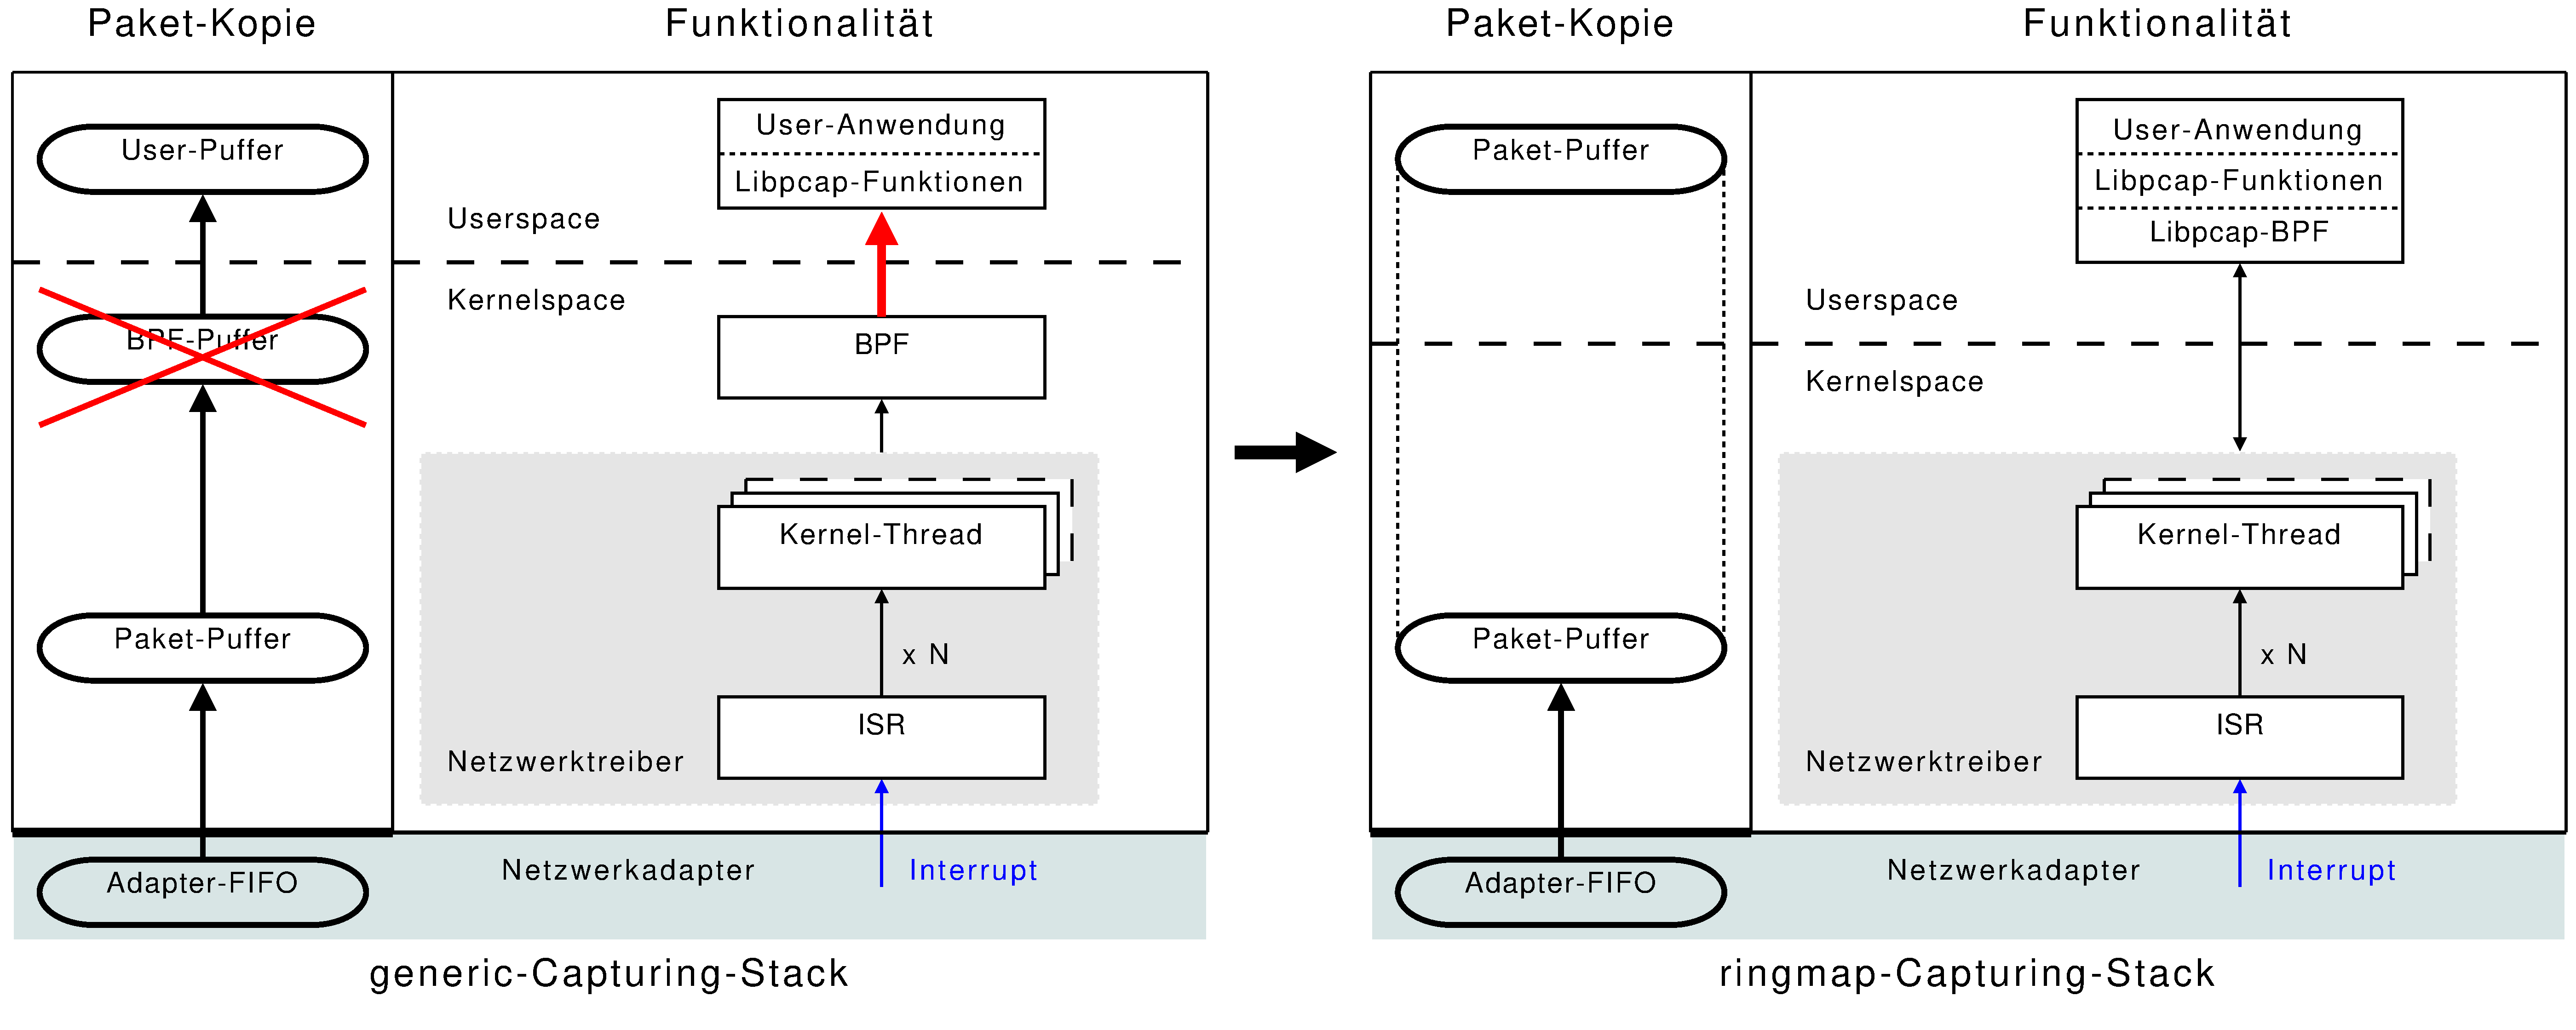
\includegraphics [height=55mm,width=115mm]{pics/Ueberblick_new}
\end{center}
\end{frame}

\section{Performance evaluation}
%%%%%%%%%%%%%%%%%%%%%%%%%%%%%%%%%%%%%%%%%%%%%%%%%%%%%%%%%%%%%%%%%%%
\begin{frame}
	\begin{center}
	\huge{Measurements and performance evaluation}
	\end{center}
\end{frame}

\subsection*{Goal of measurements}

%%%%%%%%%%%%%%%%%%%%%%%%%%%%%%%%%%%%%%%%%%%%%%%%%%%%%%%%%%%%%%%%%%%
\begin{frame}
\frametitle{Goal of measurements}
\begin{itemize}
	\item Conducting performance evaluations of \textbf{ringmap} capturing stack
		\begin{itemize}
			\item CPU-Load and packet loss during capturing\newline
		\end{itemize}
	\item Benchmarking: \textbf{generic} vs. \textbf{ringmap}
\end{itemize}
\end{frame}

%%%%%%%%%%%%%%%%%%%%%%%%%%%%%%%%%%%%%%%%%%%%%%%%%%%%%%%%%%%%%%%%%%%%
%\begin{frame}
%\frametitle{What is measured ?}
%\textbf{packet loss} and \textbf{CPU-Load} as a function of :\newline
%\begin{itemize}
%	\item Traffic parameters
%		\begin{itemize}
%			\item packet size
%			\item bit-rate and packet-rate
%		\end{itemize}
%
%\color{gray}
%	\item  Hardware components
%		\begin{itemize}
%\color{gray}
%			\item PCI vs. PCI-Express
%			\item Number of CPUs
%		\end{itemize}
%	\item Driver parameters
%		\begin{itemize}
%\color{gray}
%			\item Size of packet puffers 
%			\item etc\ldots
%		\end{itemize}
%\end{itemize}
%\normalcolor
%\end{frame}
%
%\subsection*{Testbed}
%%%%%%%%%%%%%%%%%%%%%%%%%%%%%%%%%%%%%%%%%%%%%%%%%%%%%%%%%%%%%%%%%%%%
\begin{frame}
\frametitle{Testbed}
\begin{center}
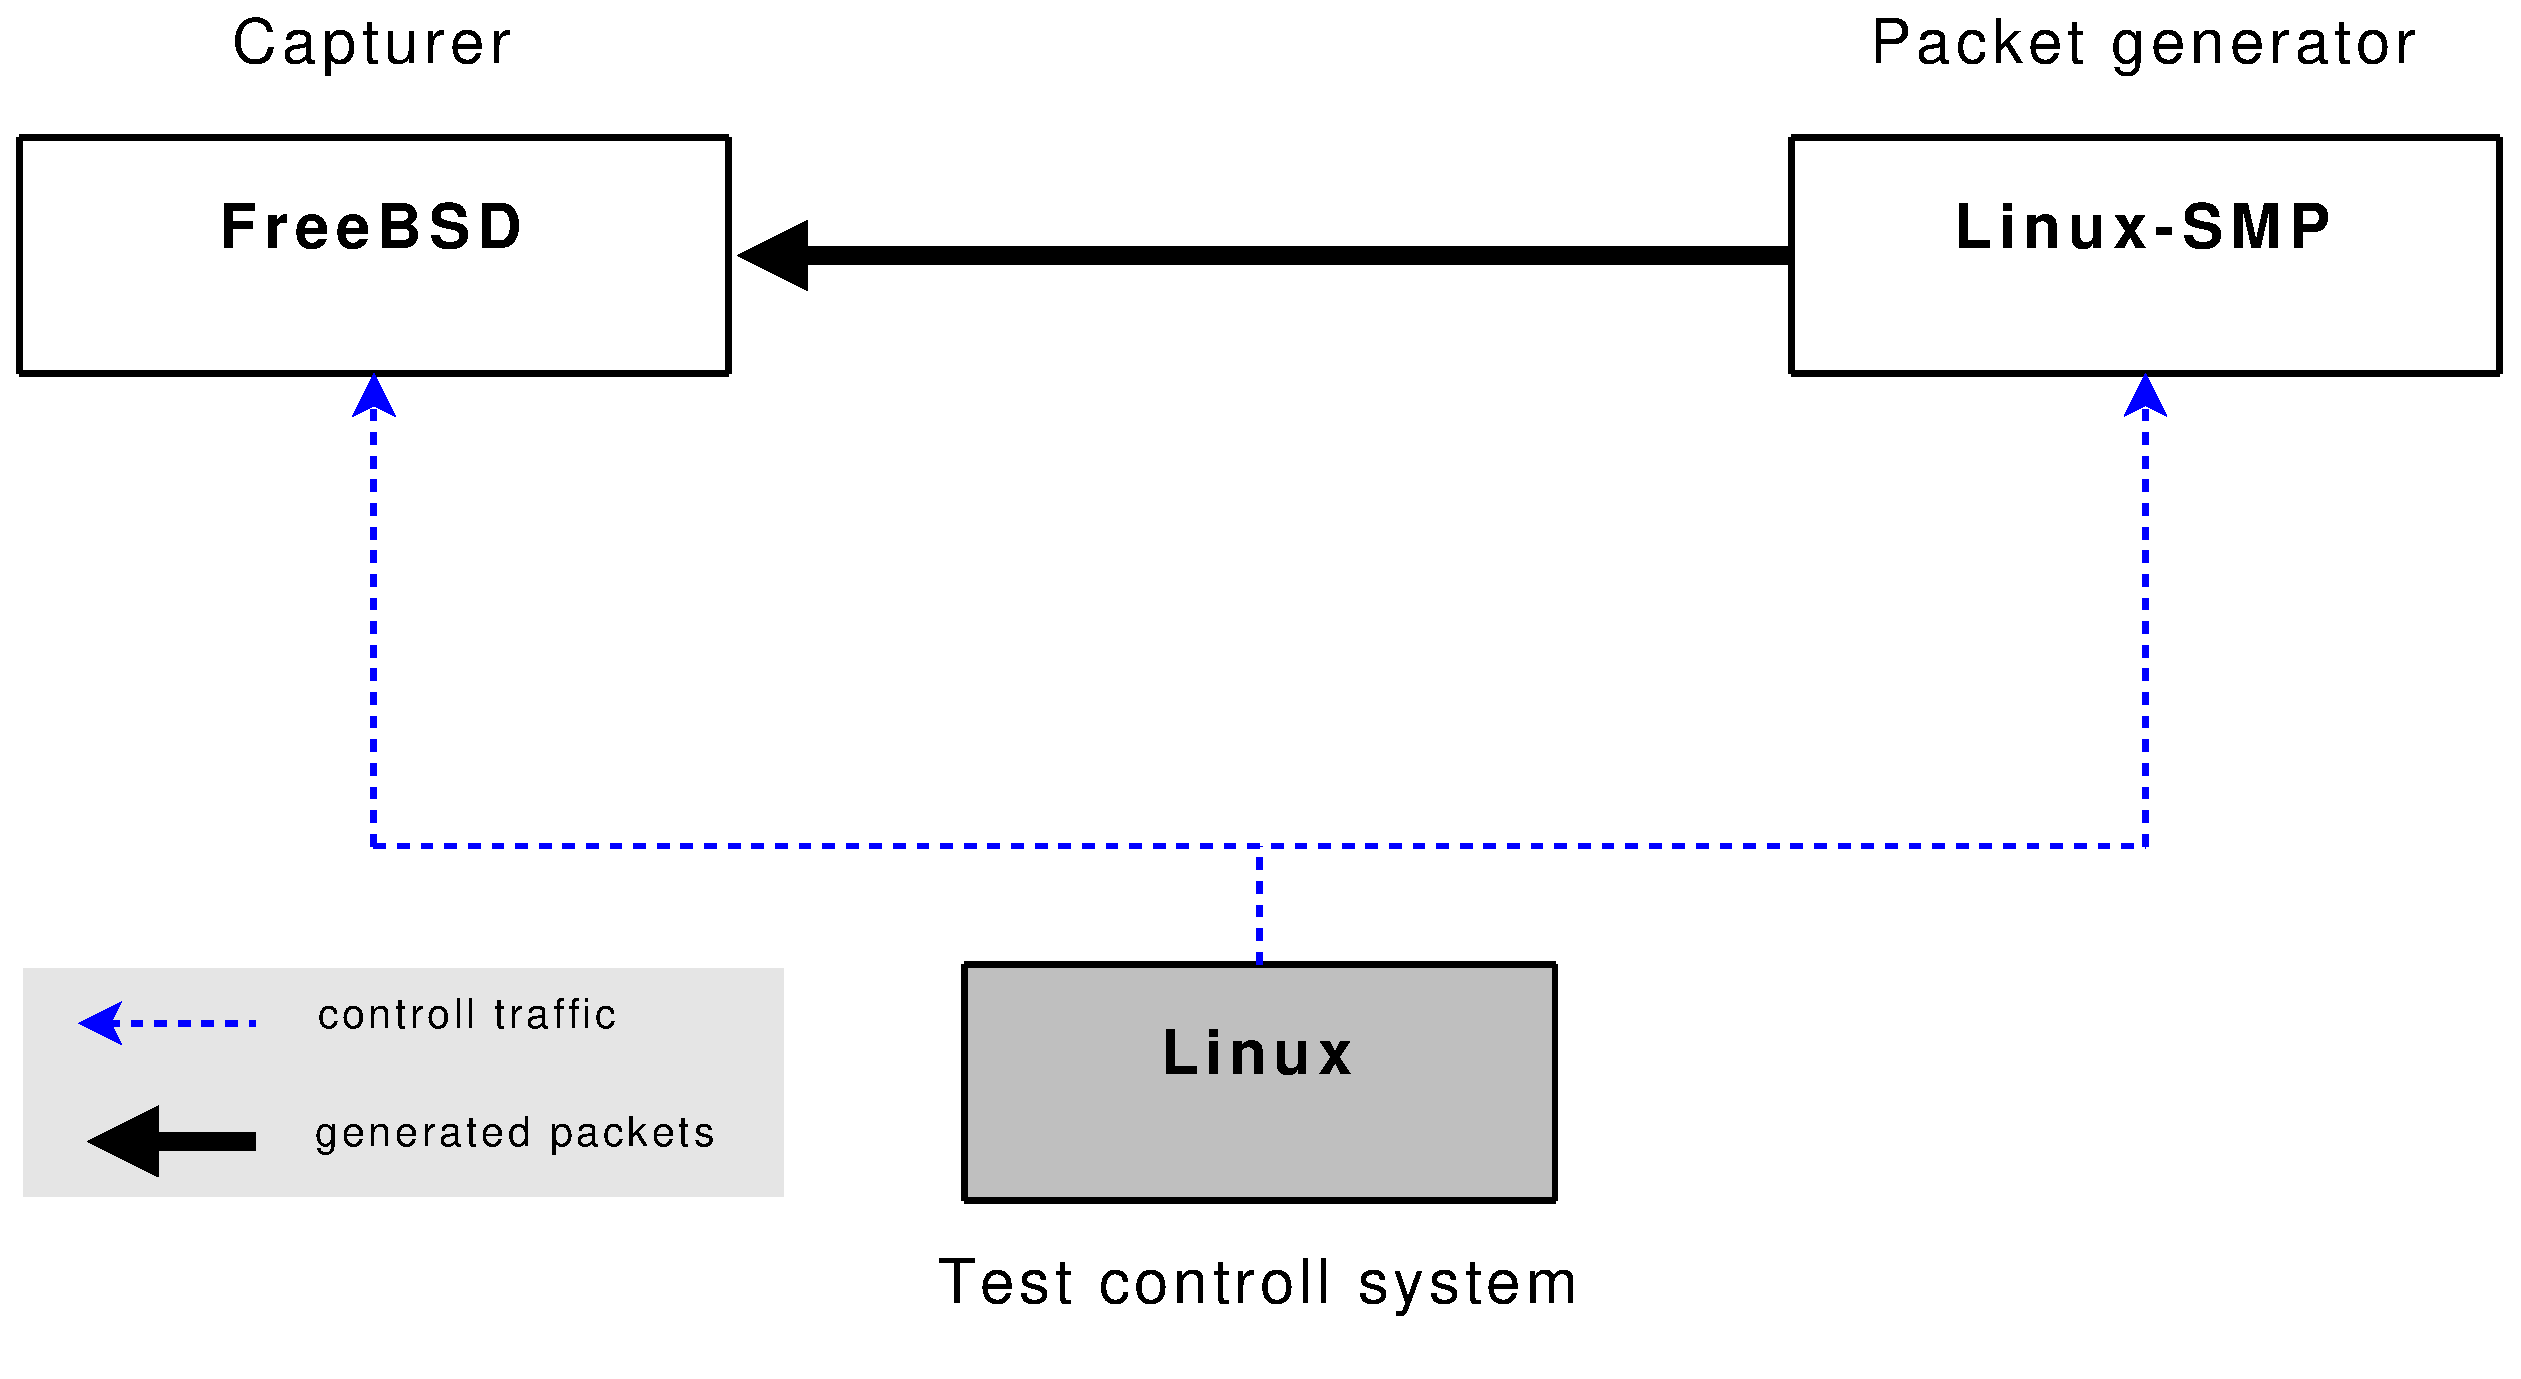
\includegraphics [height=0.68\textheight]{pics/Messaufbau}
\end{center}
\end{frame}

%%%%%%%%%%%%%%%%%%%%%%%%%%%%%%%%%%%%%%%%%%%%%%%%%%%%%%%%%%%%%%%%%%%
\begin{frame}
\frametitle{Measurement setup}
\textbf{Traffic generation}
\begin{itemize}
	\item Linux Kernel Packet Generator (\emph{pktgen})
		\begin{itemize}
			\item generates network packets at very high speed with different: 
				\begin{itemize}
					\item packet sizes
					\item bit-rate and packet-rate
				\end{itemize}
		\end{itemize}
\end{itemize}
\textbf{Capturing}
\begin{itemize}
	\item \textbf{ringmap} and \textbf{generic} stacks
	\item Libpcap-application
		\begin{itemize}
			\item accessing packets through call \emph{pcap\_loop()}
			\item counting the captured packets
		\end{itemize}
\end{itemize}
\end{frame}

\subsection*{Experiment description}


%%%%%%%%%%%%%%%%%%%%%%%%%%%%%%%%%%%%%%%%%%%%%%%%%%%%%%%%%%%%%%%%%%%%
%\begin{frame}
%\frametitle{Experiment parameters}
%For each experiment, data streams are generated with different parameters:
%\begin{itemize}
%	\item Constant parameters: 
%		\begin{itemize}
%			\item Packet size
%				\begin{itemize}
%					\item 64, 200, 300, 700, 1500
%				\end{itemize}
%		\end{itemize}
%	\item Variable parameters: 
%		\begin{itemize}
%			\item bit-rate 
%				\begin{itemize}
%					\item  $ < 1GBit/sec$
%				\end{itemize}
%		\end{itemize}
%\end{itemize}
%
%\end{frame}
%
%%%%%%%%%%%%%%%%%%%%%%%%%%%%%%%%%%%%%%%%%%%%%%%%%%%%%%%%%%%%%%%%%%%%
\begin{frame}
\frametitle{Calculation of results}
\begin{itemize}
	\item System load
		\begin{itemize}
			\item Percentage proportion of time the CPU spent in system mode
			\item Interrupt load is not considered
				\begin{itemize}
					\item because of interrupt-throttling it is always constant for \textbf{generic} and \textbf{ringmap}
				\end{itemize}
			\item $syst = 1 - intr - user - nice - idle$\newline
		\end{itemize}
	\item Packet loss
		\begin{itemize}
			\item Difference between generated and captured packets
			\item $Packets_{loss} = Packets_{send} - Packets_{received}$
		\end{itemize}
\end{itemize}
\end{frame}

\subsection*{Testing sequence}
%%%%%%%%%%%%%%%%%%%%%%%%%%%%%%%%%%%%%%%%%%%%%%%%%%%%%%%%%%%%%%%%%%%
\begin{frame}
\frametitle{Testing sequence}
\begin{enumerate}
	\item Login to the capturer to 
		\begin{itemize}
			\item start of capturing 
			\item start of system load measurement applications 
		\end{itemize}
	\item Login to the Packet-Generator to 

	\begin{itemize}
		\item generate traffic with:
				\begin{itemize}
					\item a certain number of packets
					\item a certain bit-rate and packet-rate
				\end{itemize}
	\end{itemize}

	\item Login to the capturer to 
		\begin{itemize}
			\item stop capturing- und measurement-applications
		\end{itemize}
	\item Storing of measured values
\end{enumerate}
\begin{itemize}
	\item Each experiment is repeated five times
	\item The mean and standard deviation is calculated
\end{itemize}
\end{frame}

%\subsection*{Probleme bei Experimenten}
%%%%%%%%%%%%%%%%%%%%%%%%%%%%%%%%%%%%%%%%%%%%%%%%%%%%%%%%%%%%%%%%%%%%
%\begin{frame}
%\frametitle{Problems arose in experiments }
%\begin{itemize}
%	\item Instability of  Linux Kernel Packet Generator
%		\begin{itemize}
%			\item often kernel panics
%			\item [$\Rightarrow$] therefore max. $15000000 pkts$ per experiment\newline
%		\end{itemize}
%	\item Impossible to generate traffic with any packet- or bit-rate
%		\begin{itemize}
%			\item because of Interrupt-Throttling
%			\item [$\Rightarrow$] therefore only certain measurement points \newline
%		\end{itemize}
%	\item Flow-Control
%		\begin{itemize}
%			\item limits the rate of generated traffic
%			\item [$\Rightarrow$] therefore must be switched off
%		\end{itemize}
%\end{itemize}
%\end{frame}

\subsection*{Results}
\begin{frame}
	\begin{center}
	\huge{Results}
	\end{center}
\end{frame}
%%%%%%%%%%%%%%%%%%%%%%%%%%%%%%%%%%%%%%%%%%%%%%%%%%%%%%%%%%%%%%%%%%%
\begin{frame}
\frametitle{generic vs. ringmap: Packet loss}
\begin{center}
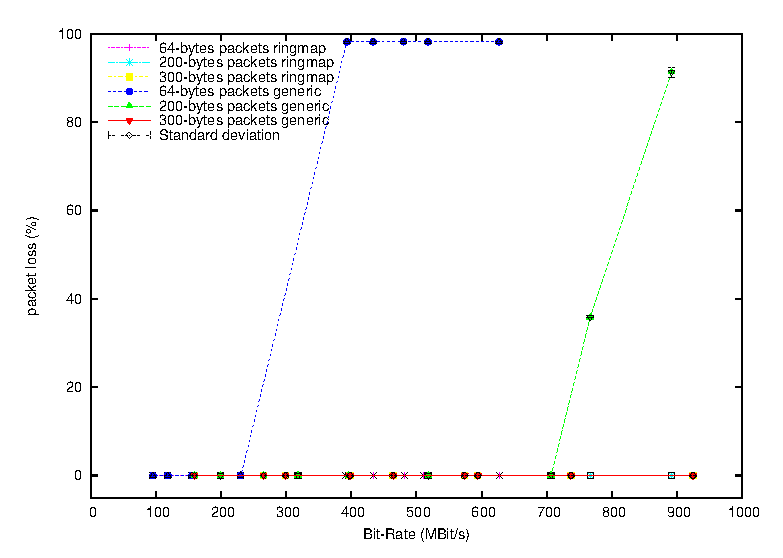
\includegraphics [height=0.81\textheight]{plots/pktloss_generic_vs_ringmap_mbs.eps}
\end{center}
\end{frame}

%%%%%%%%%%%%%%%%%%%%%%%%%%%%%%%%%%%%%%%%%%%%%%%%%%%%%%%%%%%%%%%%%%%
\begin{frame}
\frametitle{generic vs. ringmap: System-load}
\begin{center}
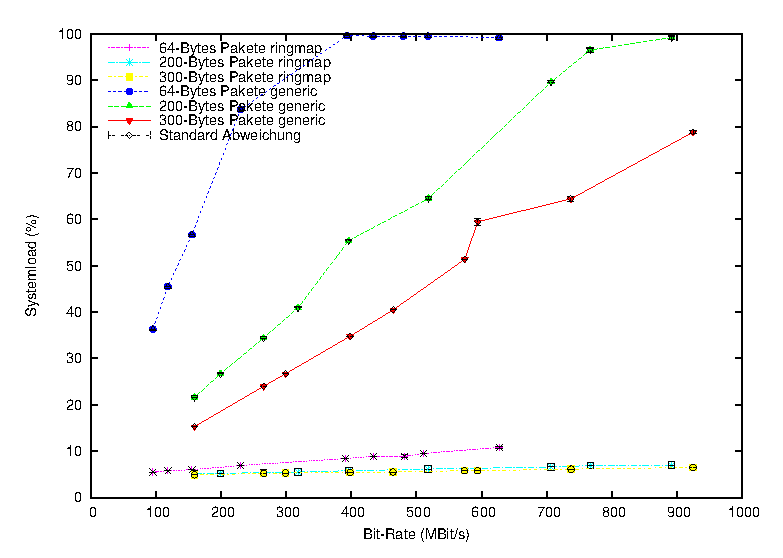
\includegraphics [height=0.81\textheight]{plots/sysload_generic_vs_ringmap_mbs.eps}
\end{center}
\end{frame}

\section{Summary}
\begin{frame}
	\begin{center}
	\huge{Summary}
	\end{center}
\end{frame}
%%%%%%%%%%%%%%%%%%%%%%%%%%%%%%%%%%%%%%%%%%%%%%%%%%%%%%%%%%%%%%%%%%%
\begin{frame}
\frametitle{Achieved goals}
\begin{itemize}
	\item \textbf{Enhanced Capturing-Performance}
		\begin{itemize}
			\item very low  system load (below $12\%$) and very low
				packet loss  (below  $0.02\%$)
				\begin{itemize}
					\item only during capturing smallest  64-Bytes packets
					\item for maximal reached packet-rate ($ > 450000 pkts/sec$)
				\end{itemize}
		\end{itemize}
	\item \textbf{Stability and usability of implemented software}
		\begin{itemize}
			\item during all experiments, no \emph{kernel panics} and no \emph{segmentation faults} occurred
			\item very simple install and remove
				\begin{itemize}
					\item two Shell-Scripts to installing  and removing the   
						\emph{ringmap} Capturing Stacks
				\end{itemize}
			\item Libpcap-applications don't require modification in order to run with the \emph{ringmap}
		\end{itemize}
\end{itemize}
\end{frame}

%%%%%%%%%%%%%%%%%%%%%%%%%%%%%%%%%%%%%%%%%%%%%%%%%%%%%%%%%%%%%%%%%%%
\begin{frame}
\frametitle{Achieved goals 2}
\begin{itemize}
	\item \textbf{Ringmap is easily portable to the other network controllers}
		\begin{itemize}
			\item The software contains hardware dependent and hardware
				independent parts. Only hardware dependent part require
				modifications.
			\item The generic driver and libpcap should contain a few hooks for calling
				\emph{ringmap}-functions.
		\end{itemize}
	\item \textbf{Packet Filtering}
		\begin{itemize}
			\item Packet filtering can be accomplished using both
				\emph{libpcap}- and kernel-BPF.
		\end{itemize}
\end{itemize}
\end{frame}
%%%%%%%%%%%%%%%%%%%%%%%%%%%%%%%%%%%%%%%%%%%%%%%%%%%%%%%%%%%%%%%%%%%
\begin{frame}
\frametitle{Achieved goals 3}
\begin{itemize}
	\item \textbf{Multithreaded Capturing}
		\begin{itemize}
			\item Multiple applications can capture from the same interface. 
		\end{itemize}
	\item \textbf{Partly ported to the 10GbE controller}
		\begin{itemize}
			\item Currently only one queue is used while capturing. The work on
				supporting multiqueue is in progress.
		\end{itemize}
\end{itemize}
\end{frame}
%%%%%%%%%%%%%%%%%%%%%%%%%%%%%%%%%%%%%%%%%%%%%%%%%%%%%%%%%%%%%%%%%%%
\begin{frame}
\frametitle{Future works}
\begin{enumerate}
	\item Benchmarking:  \textbf{Zero-Copy BPF} vs. \textbf{ringmap}
	\item Support for hardware time stamping
	\item Using TCP/IP stack together with \textbf{ringmap}
	\item 10-GbE-Paket-Capturing: Multiqueue + hardware support for packet filtering 
	\item Setting \textbf{ringmap} for packet transmission 
\end{enumerate}
\end{frame}

\end{document}
